%%%%%%%%%%%%%%%%%%%%%%%%%%%%%%%%%%%%%%%%%%%%%%%%%%%
%% LaTeX book template                           %%
%% Author:  Amber Jain (http://amberj.devio.us/) %%
%% License: ISC license                          %%
%%%%%%%%%%%%%%%%%%%%%%%%%%%%%%%%%%%%%%%%%%%%%%%%%%%

% \documentclass[a4paper,11pt]{book}
\documentclass[a4paper,11pt,openright]{book}
\usepackage{ebgaramond}
\usepackage{lipsum}
\usepackage[Lenny]{fncychap}
\ChNameUpperCase
\ChTitleUpperCase
\ChNumVar{\fontsize{40}{42}\usefont{OT1}{ptm}{m}{n}\selectfont}
% \ChTitleVar{\Large\sc}

\usepackage[T1]{fontenc}
\usepackage{booktabs}
\usepackage[utf8]{inputenc}
\usepackage{lmodern}
\usepackage{subcaption}

\usepackage{xcolor,colortbl}
\usepackage[colorlinks]{hyperref}

\def\tmp#1#2#3{%
  \definecolor{Hy#1color}{#2}{#3}%
  \hypersetup{#1color=Hy#1color}}
\tmp{link}{HTML}{800006}
\tmp{cite}{HTML}{2E7E2A}
\tmp{file}{HTML}{131877}
\tmp{url} {HTML}{8A0087}
\tmp{menu}{HTML}{727500}
\tmp{run} {HTML}{137776}
\def\tmp#1#2{%
  \colorlet{Hy#1bordercolor}{Hy#1color#2}%
  \hypersetup{#1bordercolor=Hy#1bordercolor}}
\tmp{link}{!60!white}
\tmp{cite}{!60!white}
\tmp{file}{!60!white}
\tmp{url} {!60!white}
\tmp{menu}{!60!white}
\tmp{run} {!60!white}

\definecolor{red}{rgb}{1.00,0.00,0.00}
\definecolor{blue}{rgb}{0.00,0.00,1.00}
\newcommand{\cred}[1] {\textcolor{red}{#1}}
\newcommand{\cblue}[1] {\textcolor{blue}{#1}}
\usepackage{amsmath}
\usepackage{wrapfig}    % inline figures
\usepackage{enumitem}
\usepackage{comment}
\usepackage{mathrsfs}
\usepackage{lipsum}
\usepackage{graphicx} % Use for Images
\usepackage{here}     % Forced Figure Placement
\usepackage{pslatex}	% Use PostScript Fonts
\usepackage{fancyhdr} % Use headers
\usepackage{float}
\usepackage[export]{adjustbox}
\usepackage[compact]{titlesec}
%%%%%%%%%%%%%%%%%%%%%%%%%%%%%%%%%%%%%%%%%%%%%%%%%%%%%%%%%
% Source: http://en.wikibooks.org/wiki/LaTeX/Hyperlinks %
%%%%%%%%%%%%%%%%%%%%%%%%%%%%%%%%%%%%%%%%%%%%%%%%%%%%%%%%%

\usepackage{graphicx}
\titlespacing*{\section}{0pt}{0.1\baselineskip}{0.2\baselineskip}
\titlespacing*{\subsection}{0pt}{0.1\baselineskip}{0.2\baselineskip}


% \usepackage{algopseudocode}
\usepackage{algorithm}
\usepackage{algorithmic}
\usepackage{amssymb}
\usepackage{forest}
\usepackage[english]{babel}
% \usepackage{biblatex}
\usepackage{listings}
  \lstdefinestyle{ascii-tree}{
    literate={├─}{|}1 {─}{--}1 {└}{+}1 
  }
\usepackage[
	top    = 1cm,
	bottom = 1.80cm,
	left   = 2.00cm,
	right  = 2.00cm,
	includeheadfoot]{geometry} % Use similar margins to the Word Template
\setcounter{secnumdepth}{5}
\setlength{\parindent}{0pt}
\setlist[itemize]{noitemsep, topsep=0pt}
\usepackage{setspace}\onehalfspacing\frenchspacing\flushbottom\sloppy
%      % https://tex.stackexchange.com/questions/65355/flushbottom-vs-raggedbottom

%%%%%%%%%%%%%%%%%%%%%%%%%%%%%%%%%%%%%%%%%%%%%%%%%%%%%%%%%
% Source: http://en.wikibooks.org/wiki/LaTeX/Hyperlinks %
%%%%%%%%%%%%%%%%%%%%%%%%%%%%%%%%%%%%%%%%%%%%%%%%%%%%%%%%%
\usepackage{hyperref}
\usepackage{graphicx}
\usepackage[english]{babel}
\usepackage[
backend=biber,
sorting=none
]{biblatex}
\addbibresource{My Library.bib}
\let\cleardoublepage\clearpage
\newenvironment{dedication}
{
   \cleardoublepage
   \thispagestyle{empty}
   \vspace*{\stretch{1}}
   \hfill\begin{minipage}[t]{0.66\textwidth}
   \raggedright
}
{
   \end{minipage}
   \vspace*{\stretch{3}}
  %  \clearpage
}
\definecolor{foldercolor}{RGB}{124,166,198}

\tikzset{pics/folder/.style={code={%
    \node[inner sep=0pt, minimum size=#1](-foldericon){};
    \node[folder style, inner sep=0pt, minimum width=0.3*#1, minimum height=0.6*#1, above right, xshift=0.05*#1] at (-foldericon.west){};
    \node[folder style, inner sep=0pt, minimum size=#1] at (-foldericon.center){};}
    },
    pics/folder/.default={20pt},
    folder style/.style={draw=foldercolor!80!black,top color=foldercolor!40,bottom color=foldercolor}
}

\forestset{is file/.style={edge path'/.expanded={%
        ([xshift=\forestregister{folder indent}]!u.parent anchor) |- (.child anchor)},
        inner sep=1pt},
    this folder size/.style={edge path'/.expanded={%
        ([xshift=\forestregister{folder indent}]!u.parent anchor) |- (.child anchor) pic[solid]{folder=#1}}, inner ysep=0.6*#1},
    folder tree indent/.style={before computing xy={l=#1}},
    folder icons/.style={folder, this folder size=#1, folder tree indent=3*#1},
    folder icons/.default={12pt},
}
%%%%%%%%%%%%%%%%%%%%%%%%%%%%%%%%%%%%%%%%%%%%%%%%
% Chapter quote at the start of chapter        %
% Source: http://tex.stackexchange.com/a/53380 %
%%%%%%%%%%%%%%%%%%%%%%%%%%%%%%%%%%%%%%%%%%%%%%%%
% \makeatletter
% \renewcommand{\@chapapp}{}% Not necessary...
% \newenvironment{chapquote}[2][2em]
%   {\setlength{\@tempdima}{#1}%
%    \def\chapquote@author{#2}%
%    \parshape 1 \@tempdima \dimexpr\textwidth-2\@tempdima\relax%
%    \itshape}
%   {\par\normalfont\hfill--\ \chapquote@author\hspace*{\@tempdima}\par\bigskip}
% \makeatother


% Define the page styles
\fancypagestyle{titlepage}{
	\fancyhf{}
	\fancyhead[C]{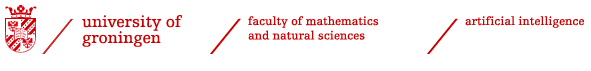
\includegraphics[width=\textwidth]{images/banner.png}}
	\renewcommand{\headrulewidth}{1pt}
}

%\fancypagestyle{body}{
%	\fancyhf{}
%  \fancyhead[C]{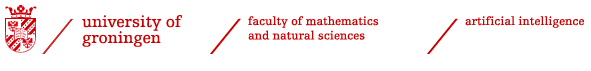
\includegraphics{images/banner.png}}
%}

\fancypagestyle{body}{
    \fancyhf{}
    % \fancyhead[C]{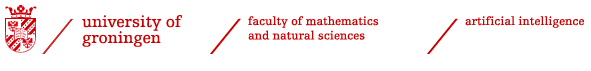
\includegraphics[width=.8\textwidth]{images/banner.png}}
    \setlength{\headsep}{8pt}
    \addtolength{\topmargin}{-45.11401pt}
    \setlength{\headheight}{77.11401pt}
    \fancyhead[LE,RO]{\thepage}
    % \renewcommand{\headrulewidth}{.4pt}
    % \renewcommand\plainheadrulewidth{.4pt}
    % \fancyhead[RE,LO]{Chapter \leftmark}
    
}
\patchcmd{\chapter}{\thispagestyle{plain}}{\thispagestyle{fancy}}{}{}

\fancypagestyle{contents}{
    % \fancyhf{}
    % \fancyhead[LE,RO]{\thepage}
    % \fancyhead[RE,LO]{\leftmark}
    \fancyhf{}
    \fancyhead[C]{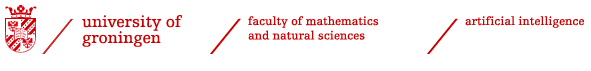
\includegraphics[width=.8\textwidth]{images/banner.png}}
    \setlength{\headsep}{1pt}
    \addtolength{\topmargin}{-45.11401pt}
    \setlength{\headheight}{77.11401pt}
    \fancyhead[LE,RO]{\thepage}
    \renewcommand{\headrulewidth}{.8pt}


}

\fancypagestyle{appendix}{
    % \fancyhf{}
    % \fancyhead[LE,RO]{\thepage}
    % \fancyhead[RE,LO]{APPENDICES}
    \fancyhf{}
    \fancyhead[C]{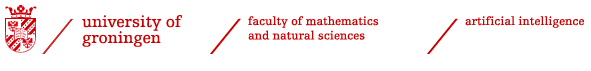
\includegraphics[width=.8\textwidth]{images/banner.png}}
    \setlength{\headsep}{1pt}
    \addtolength{\topmargin}{-45.11401pt}
    \setlength{\headheight}{77.11401pt}
    \fancyhead[LE,RO]{\thepage}
    \renewcommand{\headrulewidth}{.8pt}


}

\fancypagestyle{acknowledgements}{
    \fancyhf{}
    \fancyhead[LE,RO]{\thepage}
}


\renewcommand{\headrulewidth}{1.5pt}
\renewcommand{\arraystretch}{1.2}
\usepackage{tabularx}


%%%%%%%%%%%%%%%%%%%%%%%%%%%%%%%%%%%%%%%%%%%%%%%%%%%
% First page of book which contains 'stuff' like: %
%  - Book title, subtitle                         %
%  - Book author name                             %
%%%%%%%%%%%%%%%%%%%%%%%%%%%%%%%%%%%%%%%%%%%%%%%%%%%

% % Book's title and subtitle
% \title{\Huge \textbf{Sample Book Title}  \footnote{This is a footnote.} \\ \huge Sample book subtitle \footnote{This is yet another footnote.}}
% % Author
% \author{\textsc{First-name Last-name}\thanks{\url{www.example.com}}}
\title{
    % \vspace{1cm}
    \centering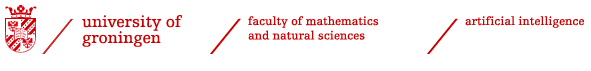
\includegraphics[width=\textwidth]{images/banner.png}
    \vspace{5mm}
        {\bf
        {\Huge Proxy Attention : Approximating Attention in CNNs using Gradient Based Techniques\\
        % \vspace{2mm}Som\\
        }
        }
        \vspace{4mm}Masters Thesis Project\\(Computational Intelligence and Robotics)\\
        \vspace{4mm}Subhaditya Mukherjee (s4747925)\\ \today \\
        \vspace{5cm}{\LARGE Internal Supervisor: S.H. Mohades Kasaei, PhD\\ Second Internal Supervisor: Matias Valdenegro, PhD}\\
        {\bf {Artificial Intelligence\\University of Groningen, The Netherlands}}
}
\date{}

\pagestyle{body}% Set page style to plain
\begin{document}
% \thispagestyle{body}
\maketitle

% \setlength{\headheight}{32pt}

% \thispagestyle{body}
\tableofcontents

% \thispagestyle{body}
\listoffigures

% \thispagestyle{body}
\listoftables


% \chapter*{Key}

\begin{enumerate}
    \item $\odot$ denotes element-wise multiplication
\end{enumerate}
% \section{Introduction}
Over the past decade or so, Computer Vision (CV) has taken over the world. Almost every domain, ranging from medicine to robotics has been affected in some way or the other because of it. At the heart of all of these improvements, reside Neural Network architectures. There are thousands of architectures, each made to serve a different purpose, some vastly better than the other. But for each of them, there exists tradeoffs. Accuracy, Memory, Time to train, Cost to run etc. Scaling up these models requires a massive amount of energy, with some consuming upwards of 27,648 kilowatt hours of electricity just to train. This is around the same amount that three households use in a whole year. \href{https://www.techtarget.com/searchenterpriseai/feature/Energy-consumption-of-AI-poses-environmental-problems}{source}. And this is just one model.\\
In order to get any kind of prediction from them, these networks need to be fed large quantities of data. This training consumes a vast amount of resources that becomes increasingly harder to provide in niche problems where only a small amount of data is available. Models that outperform existing benchmarks such as the Swin Transformer \cite{liu_swin_2022} require an abysmal amount of data and energy. This makes it extremely hard for smaller companies, research labs and individuals to use this technology.\\
The second major flaw of these systems is due to the extremely complex, high dimensional manifolds they try to model. Because of such high dimensionality, it becomes next to impossible to predict exactly why a network made the decision it did. This becomes extremely important in situations like performing medical diagnoses. Not knowing why a network said what it did, makes it very hard to trust. The rise of Explainable AI (XAI) attempts to solve this issue.\\
In order to tackle the lack of data, many methods such as transforming the present data in multiple ways to increase the available data points aka data augmentation have been created. Methods like transfer learning enable using pre-trained networks to "fine-tune" on a specific dataset. In the traditional sense, the fields of XAI and data augmentation are not related. So far, the outputs of XAI algorithms have just been used as an explainibility measure, not for training.
Therefore, combining these concepts, we arrive at a novel Augmentation technique that uses Saliency maps as an input during training to emulate Attention \cite{vaswani_attention_2017} mechanisms. We call this "Proxy Attention".\\
The objective of this thesis is to design a novel informed augmentation method that would not only reduce the requirement of data, but will also be more memory and time efficient during training as compared to current algorithms in turn building on the advances of XAI to improve training performance.
% \chapter{State of the Art}
\section{Gradient Based Explanations}
% Deconvnet
One of the earlier approaches to Saliency maps for CNNs was proposed by Zeiler et al. \cite{zeilerVisualizingUnderstandingConvolutional2013} termed DeconvNet. DeconvNet works by inverting the network's operations in the forward pass. After attaching the DeconvNet layers to the network, propagating through these layers represents features that the original CNN possessed. The relevant reconstruction can be obtained for a single class by setting all the activations other than the one corresponding to the class to zero. The resulting image is then used to generate the saliency map. A Deconv layer replaces the Conv layer, and the ReLU operation has negative values clamped. While the pooling operation is not strictly invertible, the authors use switch variables that store the maximum value position for each pooling operation. While the DeconvNet works to a certain extent, the results are less accurate than the ones obtained by other methods and are also biased towards the representations of the first layer.

% Deep Inside Conv Nets
Building on the DeconvNet, Simonyan et al. \cite{simonyanDeepConvolutionalNetworks2014} extrapolate the idea of class visualization to create one of the first approaches to Saliency maps. Their approach, also called Vanilla Gradient, ranks the pixels of an image $I_{0}$ by how important they are in the prediction of the Saliency score $S_{c}(I) \approx w^{T}I + b$. In this equation, $w$ and $b$ are the network weights and biases obtained by back-propagating wrt the image itself. The objective to be minimized thus is $arg \underset{I}max S_{c}(I) - \lambda||I||^{2}_{2}$ where $\lambda$ is used as a regularization parameter. Using these equations, a saliency map $A \in \mathbb{R}^{m \times n}$ ($m \times n$ stands for $height \times width$) can be computed. To find the map, we find the derivative of $w$, rearrange the elements and then process them according to the number of input channels. If the number of channels is greater than one, the maximum value over the channel is considered $A_{i,j}= \underset{ch}max |w_{h_{(i,j, ch)}}|$. Where $ch$ is the colour channel of the pixel $(i,j)$, $h(i,j, ch)$ is the index of the $w$ corresponding to that pixel. The Vanilla Gradient method produces an approximate saliency map but has much noise. This leads to issues for more complex images. The methods proposed in the following papers have addressed many of the issues with Vanilla Gradients and DeconvNets \cite{zeilerVisualizingUnderstandingConvolutional2013}.

% Scorecam
In another paper, the authors propose a score-weighted approach - ScoreCAM to create saliency maps \cite{wangScoreCAMScoreWeightedVisual2020}. Like many other methods, the images are first passed through the network, and the corresponding activations are obtained from the final convolutional layer. These activation maps are upsampled and normalized to $[0,1]$. The highlighted activation map portions are then passed through a CNN with a SoftMax layer to obtain the score for each of the current classes. These scores are used to find the activation maps' relative importance. Finally, the sum of all these maps is computed using a linear combination with the corresponding target score and then passed through a ReLU operation. These operations can be mathematically represented as $L^{c}_{ScoreCAM} = ReLU(\underset{k}\Sigma w_{k}^{c}A^{k})$, where $k$ represents the index considered, $c$ represents the current class and $S_k$ represents the outputs of the SoftMax as mentioned earlier layer. The authors find that the maps obtained using ScoreCAM are less noisy, and this method removes the dependency on unstable gradients compared to other methods.

% Guided Gradcam
A variant of GradCAM \cite{selvarajuGradCAMVisualExplanations} was proposed by Selvaraju et al. \cite{selvarajuGradCAMWhyDid2017} where, unlike GradCAM that finds the parts of the image that influence the model's decision, Guided GradCAM takes the positive gradients into account. These gradients are used to obtain an even more fine-grained representation of the outputs of the saliency map. While GradCAM backpropagates both positive and negative gradients, Guided Backprop only propagates the positive gradients and is defined as a pointwise multiplication of the results of GradCAM and Guided Backpropagation \cite{springenbergStrivingSimplicityAll2015}.

% Noise Tunnel
In combination with attribution methods, Noise Tunnel \cite{kokhlikyanCaptumUnifiedGeneric2020} is an algorithm that improves the accuracy of the masks obtained by these methods. Noise Tunnel was proposed to counter noisy and irrelevant attributions obtained by some gradient-based methods by adding a Gaussian Noise and then averaging the predictions over sampled attributions. Since all the samples are considered, this method has a significant computational overhead. For Smooth Grad \cite{smilkovSmoothGradRemovingNoise2017}, the new attribution is defined as $\hat M_{c}(x) = \frac{1}{n}\Sigma_{1}^{n}M_{c}(x + \mathcal{N}(0, \sigma^{2}))$. Where $M_{c}$ is the attribution calculated by SmoothGrad, $\mathcal {N}(0, 0.01^2)$ is the Gaussian Noise with $\sigma = 0.01$ and $n$ is the number of samples. Similarly for Smooth Grad Square, $\hat M_{c}(x) = \frac{1}{n}\Sigma_{1}^{n}\sqrt{M_{c}(x + \mathcal{N}(0, \sigma^{2}))}$. Noise Tunnel can also be used on Var Grad \cite{richterVarGradLowVarianceGradient2020} with the equation $\hat M_{c}(x) = \frac{1}{n}\Sigma_{k=1}^{n}\{M_{c}(x + \mathcal{N}(0, \sigma^{2}))\}^{2}- \{\hat M_{c}(x)\}^{2}$

% Integrated Gradients
For a model $F$, the attribution method Integrated Gradients \cite{sundararajanAxiomaticAttributionDeep2017} computes the contribution of each pixel in the image towards the final prediction. The model's output is used to calculate a pixel-wise partial derivative that is then integrated along a path starting from the baseline and ending at the input. Each step is scaled according to the partial derivative obtained in the previous step. For every step k with m total steps over the path, the IG equation is defined as $IntegratedGrads_i^{approx}(x)::=(x_{i}-x_i')\times \Sigma_{k=1}^{m}\frac{\partial F(x' + \frac{k}{m} \times (x-x'))}{\partial x_{i}} \times \frac{1}{m}$. Where $(x_{i} - x_{i}')$ is the pixel-wise difference between the two images, $\frac{\partial F(x' + \frac{k}{m} \times (x-x'))}{\partial x_i}$ is the partial derivative of the model output $F$ with respect to pixel $i$ at the $k$-th step of the path, and $\frac{1}{m}$ is the scaling factor that ensures that each of the steps taken contributes equally to the final result.

% Rise
Petsiuk et al. propose RISE \cite{petsiukRISERandomizedInput2018}, a saliency method that randomly alters the input images by applying random noise to each. After model predictions are obtained, the saliency map is generated by combining the partial maps over each modified image. RISE improves accuracy but needs a lot of computation time, considering that multiple models must be trained for each random noise sample.

% Influence Of Image Class Acc On Saliency Map Estimation
Oyama et al. \cite{oyamaInfluenceImageClassification2018} found a strong correlation concerning the relationship between saliency maps and image classification accuracy. The authors found that the architecture and the initialization strategy influence the final saliency map. By analyzing the generated saliency maps, they find that if the model is randomly initialized and trained for image classification, having limited categories in the original dataset leads to overfitting. On the other hand, having many categories suppresses the overfitting of the objects present in the training dataset. On training their proposed network ReadoutNet on a fixation task (which requires the network to learn where to focus), they found that the accuracy of estimating the saliency map was linked to the image classification accuracy.

% Summit
While a large amount of research focuses on interpreting the influence of a single image or neuron, Hohman et al. propose Summit, \cite{hohmanSummitScalingDeep2019} a novel scalable summarization algorithm. Summit creates an attribution graph that distils the influence of neurons and substructures throughout the network used to make the final prediction. The attribution graph is created due to combining activation aggregation, a technique to find important neurons and neuron-influence aggregation, a technique to find relationships among the neurons identified in the previous step. After a forward pass through the network, the activation channels maximums are obtained to aggregate the activations. These are then filtered by class and aggregated by taking the top $k$ channels or the top $k$ channels by weight. To quantify how much a layer influences the next, the authors aggregate the influences by creating a tensor $I^{l}$ for all the network layers ($l$). How important channel $i$ of the layer $l-1$ is determined by the aggregate tensor $I^{l}_{cij}$ where $j$ represents the output channel and $c$ is the class of the image. Considering the $j^{th}$ kernel of the layer $K^{(j)} \in \mathbb{R}^{H \times W \times C_{l-1}}$, a single channel $Y$ can be represented using the 3D convolution operation by $Y_{:,:,j}= X \ast K^{(j)}$. This is equivalent to it's representation by the 2D convolution $Y_{:,:,j}= \Sigma_{i=1}^{C_{l-1}} X_{:,:,i} \ast K^{(j)}_{:,:,i}$. The value $X_{:,:,i} \ast K^{(j)}_{:,:,i}$ is the contribution of the current channel from the previous layer and the maximum of this value is used to generate the influence map.

% Conductance
Building upon Integrated Gradients, Dhamdhere et al. propose \cite{dhamdhereHowImportantNeuron2018} Conductance, a means to boost the attributions provided by IG to specific neurons in the hidden layer. This is done by decomposing the computation that IG performs. The authors apply this method to the Inception network \cite{szegedyGoingDeeperConvolutions2014} and can find the filters that influence the final predictions most. 
For a neuron $y$ , the network can be represented as a function $F:R^{n} \rightarrow [0,1]$. Given an input $x \in R^{n}$ and a baseline input $x' \in R^{n}$, the IG for the $i^{th}$ dimension at $x$ is given by $IG_{i}(x) ::== (x_{i}- x_{i}') \int_{\alpha=0}^{1} \frac{\partial F(x' + \alpha(x-x'))}{\partial x_{i}}d \alpha$ . Considering $\frac{\partial F(x)}{\partial x_{i}}$ to be the gradient of $F$ along $i^{th}$ dimension at x, the Conductance for $y$ can be defined as $
Cond_{i}^{y}(x) ::== (x_{i}- x_{i}') \int_{\alpha=0}^{1} \frac{\partial F(x' + \alpha(x-x'))}{\partial y} \cdot \frac{\partial y}{\partial x_{i}} d \alpha$. The authors also propose methods of evaluating Conductance by the assumption that an influential hidden network should be good at predicting the given input class. This assumption can be validated by two metrics : the $Gradient\times Activation$ : $
y \times \frac{\partial F(x' + \alpha \times (x-x'))}{\partial y} d \alpha$ and the Internal Influence : $
IntInf ^{y}(x) ::= \int^{1}_{\alpha=0} \frac{\partial F(x' + \alpha(x-x'))}{\partial y} d \alpha$.\\

% Smooth Grad
Consider an image classification task where an input image $x$ is classified as a single class from a set $C$. For every class $c \in C$, the output class is represented as $class(x) = argmax_{c \in C}S_{c}(x)$. Using this $class$, a sensitivity map $M_{c}(x)$ can be generated by differentiating with respect to $x$, $M_{c}(x) = \frac{\partial S_{c}}{\partial x}$ . $M_{c}$, being a sensitivity map (\cite{simonyanDeepConvolutionalNetworks2014}), thus representing the influential regions of the image used to make the prediction. Since these maps are noisy, Smilkov et al. propose SmoothGrad \cite{smilkovSmoothGradRemovingNoise2017}, a modification of the previous method where instead of using $\partial S_{c}$, a smoothing is applied using a Gaussian kernel to $\partial S_{c}$. The authors also find that it is impossible to directly compute the smoothing due to high dimensionality and thus approximate the calculation by averaging multiple maps computed in the neighbourhood of $x$ using random sampling. The final SmoothGrad equation then becomes $\hat M_{c}(x) = \frac{1}{n}\Sigma_{1}^{n}M_{c}(x + \mathcal{N}(0, \sigma^{2}))$, where $\mathcal{N}(0, \sigma^{2})$ is the Gaussian noise and $\sigma$ is the standard deviation.

Deep Lift

Deep Visual Explanations

% Embedding Knowledge Into Deep Attention Map
- method for embedding human knowledge into deep neural networks
- challenging to apply it for deep learning models due to the enormous number of model parameters
- we focus on the attention mechanism of an attention branch network (ABN).
- fine-tuning method that utilizes a single-channel attention map which is manually edited by a human expert
- Our fine-tuning method can train a network so that the output attention map corresponds to the edited ones
- the fine-tuned network can output an attention map that takes into account human knowledge
- We demonstrate that manually editing the attention map used for a visual explanation can improve the recognition performance by reflecting human knowledge
- By training a network to output the same attention maps as the edited ones, we can embed human knowledge into deep neural networks
- this paper formulates a novel optimization framework of networks that humans can intuitively edit via a visual interface
- We first input a misclassified sample to ResNet152+ABN and obtain the attention map from the attention branch, where the size of the attention map is 14×14 pixels. Then, we edit the obtained attention map manually. Note that the attention map is resized to 224×224 pixels and is overlaid with the input image for ease of manual editing. The edited attention map is resized to 14 × 14 pixels and used for an attention mechanism to infer classification results from the perception branch
- tool that can edit attention maps interactively
- This tool can add (Fig. 5(a)) and remove (Fig. 5(b)) an attention region simply by dragging the mouse
- During the fine-tuning, the proposed method optimizes the attention and perception
- branches of ABN. The feature extractor that extracts the feature map from an input image is not updated during the fine-tuning process.

Sam Resnet

Cam

Gradcam++

Guided Backprop

Salience Map



\section{Augmentation} \label{sec:augmentation}
% Augmix
Another augmentation strategy proposed by \cite{hendrycksAugMixSimpleData2020} first applies multiple transformations randomly and in parallel chains to each image. These transformations can include combinations of Translation, Rotation, Shearing and others. The outputs of these combinations are then mixed to form a new image, which is further mixed with the original image to form the new image. This combination improves performance in cases where data shifts are encountered in production. Once the images are mixed, a skip connection is used to combine the results of the chains. AugMix also uses the Jensen-Shannon Divergence consistency loss \cite{linDivergenceMeasuresBased} to ensure the images are stable across various inputs. Considering $KL$ to be Kullback-Leibler Divergence, the Jensen-Shannon Divergence can be defined as $
    JS(p_{orig}; p_{augmix1};p_{augmix2}) = \frac{1}{3}(KL[p_{orig}||M||]+KL[p_{augmix1}||M||]+KL[p_{augmix2}||M||])
$, where $M$ is the mean of the three distributions $p_{orig}, p_{augmix1}, p_{augmix2}$.

% Cutout
Devries et al., in their paper \cite{devriesImprovedRegularizationConvolutional2017}, propose an augmentation method they call Cutout. This method removes random-sized square patches from the images by replacing the corresponding pixels with a constant value (usually 0). Selecting the region involves picking a random pixel value and creating a uniform-sized square around the chosen pixel. The authors also find that Cutout performs better with other methods than just being used by itself. Cutout can be expressed as an element-wise multiplication operation $x_{cutout} = x \odot M$,
$x$ is the original image, $M$ is a binary mask of the same size as $x$ with randomly chosen coordinates of a square patch of pixels to be cut out, and $\odot$ denotes element-wise multiplication.

% Cut and mix
Unlike Cutout \cite{devriesImprovedRegularizationConvolutional2017}, where the chosen patch is replaced with zero pixels, in CutMix \cite{yunCutMixRegularizationStrategy2019}, the chosen patch is replaced with a randomly chosen patch from a different region of the same image. Yun et al. propose this approach as multiple class labels can be learned with a single image.
CutMix can be defined by the following operations $\overset{\sim}x = M \odot x_{A} + (1-M) \odot x_{B}$ ; $\overset{\sim}y = \lambda y_{A}+ (1- \lambda)y_{B}$. $x$ is an RGB image, $y$ is the respective label, $M$ is a binary mask of the image patch that will be dropped, and $\odot$ represents element-wise multiplication. The new training sample $\overset{\sim}x , \overset{\sim}y$ is created by combining two other training samples $x_{A}, y_{A}$ and $x_{B} , y_{B}$. To control the combination ratio $\lambda$, a sample from the $\beta(1,1)$ distribution is chosen. This combination is quite similar to \cite{zhangMixupEmpiricalRisk2018} but differs in the sense that CutMix focuses on generating locally natural images.
% \nolinebreak
% Attentive Cutmix
Building upon \cite{yunCutMixRegularizationStrategy2019}, Walawalkar et al. propose an alternative method of replacing patches in an image they call Attentive CutMix \cite{walawalkarAttentiveCutMixEnhanced2020}. Instead of randomly pasting patches in the image, this method uses a pre-trained network to identify attentive regions from the image. Similar to the earlier approach, these patches are mapped back to the original image. Doing so allows the network to select important background regions for the task while also updating the label information.

% Cow Mask
Many of the algorithms use rectangular or square-shaped masks. While effective, French et al. propose Cow Mask \cite{frenchMilkingCowMaskSemiSupervised2020}, a new masking method that uses irregularly shaped masks with a Gaussian filter to reduce noise. The authors also propose two mixing methods, one that builds up on Random Erasing \cite{zhongRandomErasingData2020}, and another that uses Cut Mix \cite{yunCutMixRegularizationStrategy2019}. A pixel-wise mixing threshold is also chosen, and either mixing or erasing is applied to the image based on this threshold. This augmentation technique is shown to be effective in semi-supervised learning.

% Cut Paste Learn
\ proposed another approach involving a cut-paste methodology cite{dwibediCutPasteLearn2017}. In their paper, the authors propose a new method of augmentation that extracts instances of objects from the images. Instead of pasting them on other images, they are pasted on randomly chosen backgrounds. This method leads to pixel artefacts in the images, as selecting the objects is a noisy process. To overcome the drop in performance, the authors apply a Gaussian blur and Poisson blending to the boundaries of the pasted objects. Further augmentation is applied before pasting the objects by rotation, occlusion and truncation. The authors also find that this approach makes the network more robust to image artefacts.

% Hide and Seek
In their paper, Singh et al. \cite{singhHideandSeekDataAugmentation2018} propose a data augmentation method that takes an image as an input and divides it into a grid. Each of the sub-grids is then turned off with a given probability. These sub-grids can be connected or independent of each other, and the turned-off grids are replaced by the average pixel value of all the images in the dataset.

% GridMask
One of the major drawbacks of algorithms that rely on modifying image patches (such as \cite{singhHideandSeekDataAugmentation2018,devriesImprovedRegularizationConvolutional2017,zhongRandomErasingData2020}) is that they sometimes delete parts of the image that might be useful to the network. To overcome this problem, Chen et al. propose a new method Grid Mask \cite{chenGridMaskDataAugmentation2020}, that uses evenly spaced grids to find a balance between the amount of information that is deleted and stored. Using the number of grids and their respective sizes as a hyperparameter, the authors find that Grid Mask effectively preserves important parts of the image.

% Intra-class part swapping
Zhang et al. propose another data augmentation method that uses a CAM \cite{zhouLearningDeepFeatures2016} to identify the most important regions of an image. These parts are then thresholded, scaled, translated and pasted onto the target image. A similar process is also applied to the target image, and the attentive parts of the original image are used to replace the corresponding attentive parts of the target image. Similar to previous methods, the labels are also updated to reflect the changes in the image.

% Random Erasing
While Cutout augmentation \cite{devriesImprovedRegularizationConvolutional2017} is applied to every image in the dataset, Zhong et al. propose a new method, Random Erasing, that takes a probability of being applied into account \cite{zhongRandomErasingData2020}. In Random Erasing, contiguous rectangular regions are selected and replaced randomly with random upper and lower limits chosen for both region area and aspect ratio. A region-aware detection algorithm is applied for object detection tasks to make the network more robust to occlusion. Note that Cutout removes square patches, while Random Erasing removes square or rectangular patches.

% Resizemix
Many augmentation methods that rely on randomly choosing regions to cut and paste from sometimes fail to work well with regions that need more object information. ResizeMix \cite{qinResizeMixMixingData2020} tackles this problem by replacing the patch with a proportionally resized version of the selected image. This method is similar to CutMix \cite{yunCutMixRegularizationStrategy2019} but differs in the sense that ResizeMix uses a resized version of the entire image instead of a randomly chosen patch.

% Ricap
Another augmentation technique that applies random cropping and pasting is RICAP \cite{takahashiDataAugmentationUsing2020}. In this method, four regions are cropped from different images and pasted together to form a new image. The created image thus has multiple mixed labels. A uniform distribution is used to determine the area of each cropped region in the final image. The authors propose multiple variants of RICAP that use different points of origin for cropping. The method works best when the cropped regions use the corners as the origin, allowing the network to see more of the image.

% Sample pairing
In their paper, Inoue et al. propose a method that merges images not by cut and paste but by averaging their pixel intensities. While algorithms like Mixup \cite{zhangMixupEmpiricalRisk2018} modify the image's labels proportional to the amount of mixing between the original and the target images, Sample Pairing \cite{inoueDataAugmentationPairing2018} maintains the same training labels. Sample Pairing follows an interval-based augmentation policy, where the network is trained for 100 epochs before being introduced to the mixed images. This process is also repeated cyclically with eight epochs of training with mixed images followed by 2 epochs of training with normal images.

% Smooth mix
With the success of mask-based approaches for data augmentation, there have been many papers that attempt to fix the flaws of previous research. One such method is SmoothMix \cite{leeSmoothMixSimpleEffective2020}, which builds up on both CutMix \cite{yunCutMixRegularizationStrategy2019} and Cutout \cite{devriesImprovedRegularizationConvolutional2017} but modifies the mask to have softer edges. The intensity of the masked edges gradually decreases and depends on the strength of the mask. The updated pixel values are thus obtained by mixing the mask with the original image according to the formula $\lambda= \frac{\Sigma_{i=1}^{W}\Sigma_{j=1}^{H}G_{ij}}{WH}$. Where $G_{ij}$ is the pixel value of mask $G$ and $H,W$ are the height and width of the image, respectively. The new pixel values are then $(x_{new} , y_{new}) = (G.xa + (1 - G).xb , \lambda.ya + (1 - \lambda).yb)$

% Smote
One of the older data augmentation methods is SMOTE \cite{SMOTESyntheticMinority}. This algorithm is not domain specific, but in the context of computer vision, it can be used to balance datasets that suffer from imbalanced labels. SMOTE generates new samples by combining the K-nearest neighbours of the minority class images to form new instances. Although many of the other methods discussed in this paper are more effective, SMOTE is still useful.

% Snap mix
Huang et al. propose SnapMix \cite{huangSnapMixSemanticallyProportional2021}, where choosing the patch size to be cut is determined from the beta distributions of both the original and target images. The extracted patches are then merged with random image regions, each of which is different in size. Labels are also updated by taking the composition of the images into account.
% Remix
Cao et al. address the problem of class imbalance by performing data augmentation on images that are part of a minority class. From the labels of the images that were mixed, the final label is chosen as the label of the image with the least representation in the dataset. The authors call this method ReMix \cite{caoReMixImagetoImageTranslation2021}.
% Visual context Augmentation
Dvornik et al. propose Visual Context Augmentation \cite{dvornikModelingVisualContext2018} that uses a NN to understand the context of objects in the image before pasting them in the target image. The authors generate training data by first generating pairs of context images with the objects masked out. These images are then fed into the NN to learn the difference between objects and backgrounds given the masked pixels. Once the model has learnt this information, instances of the objects are placed into the masked regions of the target image.

% Puzzle mix
While many techniques are based on Mixup \cite{zhangMixupEmpiricalRisk2018}, they are mostly focused on generating new samples of images from the existing data. Doing so is useful but sometimes leads to generating examples that confuse the network and do not represent the data. To tackle this issue, Kim et al. \cite{kimPuzzleMixExploiting2020} propose Pizzle Mix, an algorithm that learns to copy patches of images between each other while taking saliency into account. Puzzle Mix learns to minimize the equation $h(x_{0}, x_{1}) = (1-z) \odot \Pi_{0}^{T}x_{0} + z \odot \Pi_{1}^{T}x_{1}$ where $x_{0}, x_{1}$ are the two images, $z_{i}$ is a binary mask, $\lambda = \frac{1}{n}\Sigma_{i}z_{i}$ is the mixing ratio and $\Pi_{0}, \Pi_{1}$ represent $n \times n$ grids that denote the amount of mass that is transported during transport of the image patch to another location. 

% liuDataAugmentationLatent2018
Liu et al. \cite{liuDataAugmentationLatent2018} propose a method LSI, that uses an adversarial autoencoder to impose a uniform distribution on the latent space. The authors then perform linear interpolation on the latent space to generate new samples. This method is a modification of Mixup \cite{zhangMixupEmpiricalRisk2018}, where the linear interpolation is performed in the latent space instead of the pixel-level. This new augmentation technique overcomes the limitation of previous methods that can generate only a small set of new data given an existing image. Many of the other methods rely on random sampling and linear interpolation, which can result in finding samples that are far away from the required parts of the data manifold. Since vision datasets are very high dimensional, this is a common problem that the authors address. The authors use one-hot vectors to label the original samples. The final loss is a weighted sum ($\lambda$) of the cross-entropy losses of the generated samples with their original samples. If $\lambda$ equals 0.5, a two-hot vector is used for labels. This method performs well on smaller datasets, such as classifying medical images.

% Randaugment
- \cite{cubukRandaugmentPracticalAutomated2020}
- Commonly, a smaller proxy task is used to overcome the expense of the search phase, but it is not clear if the optimized hyperparameters found on the proxy task are also optimal for the actual task.
- The process of designing automated augmentation strategies is being rethought.
- It is proposed to only search for a single distortion magnitude that jointly controls all operations, which reduces computational expense and eliminates the need for a separate proxy task.
- RandAugment, uses a parameter-free procedure of always selecting a transformation with uniform probability from a set of K=14 available transformations
- and a single distortion magnitude that jointly controls all operations.
- The reason we wish to remove the search phase is because a separate search phase significantly complicates training and is computationally expensive.
- In order to remove a separate search phase, we aspire to fold the parameters for the data augmentation strategy into the hyper-parameters for training a model.
- RandAugment is largely insensitive to the selection of transformations for different datasets.
- We see that while [[geometric transformations]] individually make the most difference, some of the color transformations lead to a degradation of validation accuracy on average
transformation with a parameter-free procedure of always selecting a transformation with uniform probability $\frac{1}{K}$ 
- Given N transformations for a training image, RandAugment may thus express $K^{N}$ potential policies.
- magnitude of the each augmentation distortion.
- Briefly, each transformation resides on an integer scale from 0 to 10 where a value of 10 indicates the maximum scale for a given transformation
- A data augmentation policy consists of identifying an integer for each augmentation.
- and postulate that a single global distortion M may suffice for parameterizing all transformations
- We experimented with four methods for the schedule of M during training: constant magnitude, random magnitude, a linearly increasing magnitude, and a random magnitude with increasing upper bound

\subsection{Similar Methods}
- Some papers have similar ideas, different domains
- This section explains how they are different from our method

% M2Det
- \cite{zhaoM2DetSingleShotObject2019}
- The Multi-level Feature Pyramid Network has similar ideas but does not use the outputs of [[XAI]] algorithms. 
- This uses channel wise attention : ours is independant of that
- This takes images and passes them through multiple networks and then aggregates the features obtained from each of those networks. : ours uses a trained network and is independent of all that. Unlike the former, ours does not use a compressed feature map but uses a trained network to predict an explainability map instead.

% Saliency Mix
- \cite{uddinSaliencyMixSaliencyGuided2021}
- Similar to CutMix \cite{yunCutMixRegularizationStrategy2019}
- extracts salient regions and pastes them on the corresponding location in the target image
- The salient region is extracted around the maximum intensity pixel location in the saliency map
- selects a representative image patch with the help of a saliency map and mixes this indicative patch with the target image
- models that are trained with SaliencyMix help to improve the object detection performance
- It first extracts a saliency map of the source image to highlight the objects of interest and then selects a patch surrounding the peak salient region to mix with the target image.
- Another image $I_{s} \in \mathbb{R}^{W \times H \times C}$
    - $I_{a} = M \odot I_{s} + M' \odot I_{t}$
	- $M \in \{0,1\}^{W, H}$
    - labels $y_{a} = \lambda y_{t}+ (1-\lambda)y_{s}$
- Different from Proxy Attention.
    - Proxy attention does not mix images and labels, instead uses the attention map to re-weight the image 
    - More schedules and hyperparameters to tune

% Keep augment
- cite \cite{gongKeepAugmentSimpleInformationPreserving2021}
- standard augmentation may introduce distribution shifts
- increase fidelity of the augmented data
- use saliency maps to identify the regions of interest, then make sure those regins are not affected by the augmentation
- Selective Cut
    - Randomly sample regions $S$ to be cut until importance score $\mathcal{I}(S, x, y)$ is smaller than threshold $\tau$ 
    $$
    \tilde x= (1-M(S)) \odot x$$
    - where $M(S) = |M_{ij}(S)|_{ij}$ is the binary mask for $S$, $M_{ij} = \mathbb{I}((i,j) \in S)$
- Selective Paste
    - image level augmented data $x' = \mathcal{A}(x)$ , uniformly sample region $S$ that satisfies $\mathcal{I}(S,x,y) > \tau$ for a threshold $\tau$ 
    - paste the region $S$ of the original image  $x$ to $x'$ 
        - $$\tilde x = M(S) \odot x + (1-M(S)) \odot x'$$
        - $M_{ij}(S) = \mathbb{I}((i,j) \in S)$ is the binary mask of the region $S$
- Efficiency 
-  Low Resolution Based Approximation
    - we proceed as follows: a) for a given image x, we first generate a lowresolution copy and then calculate its saliency map; b) we map the low-resolution saliency maps to their corresponding original resolution
    - This allows us to speed up the saliency maps calculation significantly, e.g., on ImageNet, we achieve roughly 3× computation cost reduction by reducing the resolution from 224 to 112.
- Early Classification Head Based Approximation
    - In practice, we add an additional average pooling layer and a linear head after the first block of our networks evaluated
    - We achieve about 3× computation cost reduction in computing saliency maps
- Different from Proxy
 - Use the saliency map to ensure that the regions of interest are not affected by the augmentation , instead of using this information to help the network understand the image
 - Meant to work properly with standard augmentation techniques, instead of stand alone

\subsection{Limitations}
While each of these papers has its strengths, a few limitations were identified. These limitations do not affect the methods themselves but rather how they are used in the project context.
\begin{itemize}
    \item Most of the algorithms are used as a final post-processing of the outputs to find the inherent biases present in the network. While this is the most common use case, it does not influence the network to learn from its mistakes and improve its performance. The XAI methods generally focus on explaining the network's decisions rather than improving them. This research proposes performing the latter.
    \item Contextual awareness in image classification is difficult to achieve without special networks or longer training times. While object detection tasks require this knowledge, networks trained purely for classification can do without it. That being the case, most of the research surveyed tackles this challenge in ways that are not generalizable to other networks easily. Proxy Attention, conversely, is independent of the network and can be used with any model and dataset. 
    \item Combining the fields of XAI and data augmentation to improve network performance is a rare practice. This research is performed to bridge the gap between the two fields and to show that they can be used together to improve not only the performance of the network but also the explainability of the network's decisions simultaneously.

\end{itemize}
% 
\chapter{Implementation}
\section{Overview}
\section{Hyper parameters}
\subsection{Clear Every Step}

\subsection{Gradient Method}

\subsection{Gradient Threshold Considered}

\subsection{Multiply Weight }

\subsection{Proxy Steps}

\subsection{Subset Of Wrongly Classified}

\section{Data Loading and Pre Processing}
\subsection{Directory structure}

\subsection{Label function}

\subsection{Clearing proxy images}

\subsection{Encode, Stratify, Kfold}

\subsection{train and test, val separate}

\subsection{Augmentations}
Imagenet Normalize
Tensor
Num workers

\section{Training Details}

\section{Grid Search}

\section{Optimizations}
\subsection{Mixed Precision}
\subsection{Gradient Scaling}
\subsection{No grad}
\subsection{Batched Proxy step}
\subsection{Trial Resumption}


\subsection{Models}
TIMM

\section{Gradient Based Methods}
\section{Proxy Attention}
\subsection{Callback Mechanism}
\section{Tensorboard}
\section{Transfer learning}
\section{Optimizer}
\section{LR scheduler}
\section{Loss function}
\section{Batch sizer finder}
\section{Result Aggregation}

\section{Inference}
%\chapter{Results} \label{ch:results}
% \section{Metric Based Analysis}
% \section{Visual Based Analysis}
In line with the research questions, the evaluation section aims to quantify the performance gains obtained by using the Proxy Attention method. The section will compare the performance of networks that were trained with, and without Proxy Attention on the basis of classification metrics, and explainability improvements.

Note that complete performance logs can be found in the appendix.
\section{Accuracy}
This section explores the validation accuracy obtained by the models for different hyperparameters and datasets. Since the task at hand is a classification task, this measure is a direct comparison of the performance of the models.

\subsection{Results Per Dataset}
This subsection shows the accuracies per model for each dataset. Tabulated results can be found in the appendix in Table ~\ref{tab:summary_ds}.

\subsection{Tsing Results}
This section shows the accuracies per model for the Tsing dataset. The results are shown in Figure \ref{fig:tsing_results}. 
\begin{figure}[H]
    \centering
    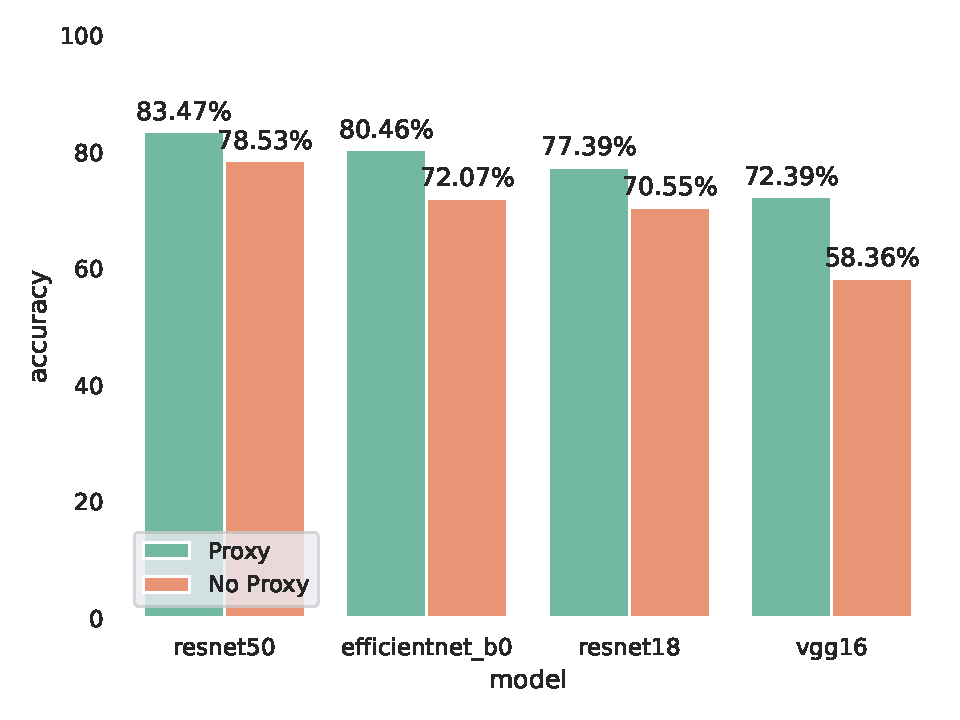
\includegraphics[width=1\textwidth]{results/tsing_results.pdf}
    \caption{Comparing Accuracies of models trained with and without Proxy Attention on the Tsing dataset}
    \label{fig:tsing_results}
\end{figure}

\subsection{Places256 Results}
This section shows the accuracies per model for the Places256 dataset. The results are shown in Figure \ref{fig:places256_results}. 
\begin{figure}[H]
    \centering
    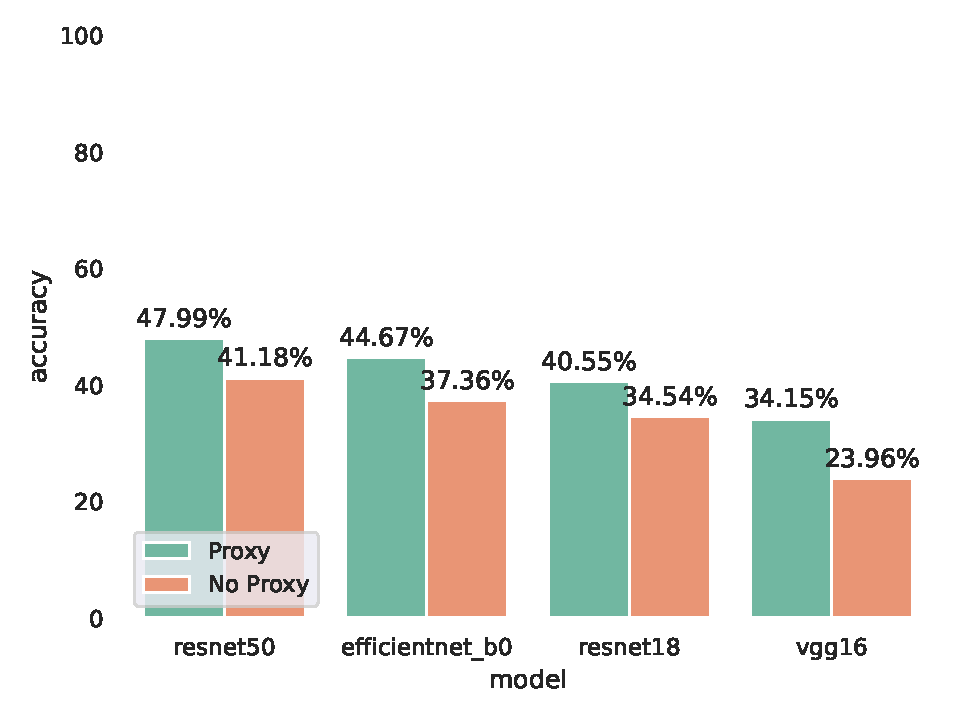
\includegraphics[width=1\textwidth]{results/places256_results.pdf}
    \caption{Comparing Accuracies of models trained with and without Proxy Attention on the Places256 dataset}
    \label{fig:places256_results}
\end{figure}

\subsection{Dogs Results}
This section shows the accuracies per model for the Dogs dataset. The results are shown in Figure \ref{fig:dogs_results}. 
\begin{figure}[H]
    \centering
    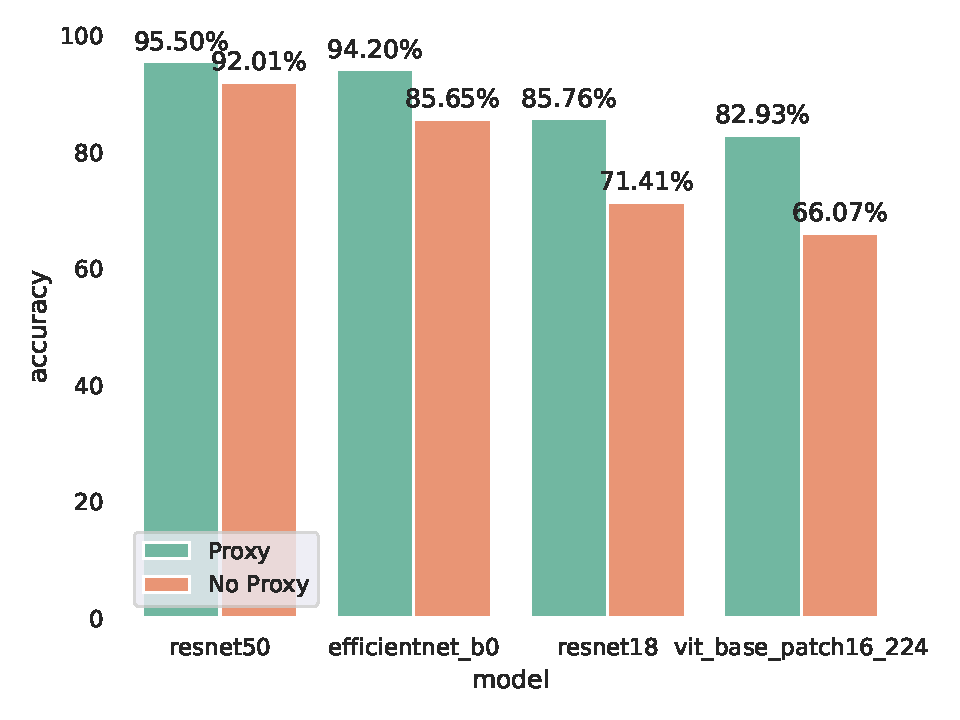
\includegraphics[width=1\textwidth]{results/dogs_results.pdf}
    \caption{Comparing Accuracies of models trained with and without Proxy Attention on the Dogs dataset}
    \label{fig:dogs_results}
\end{figure}

\subsection{Cifar100 Results}
This section shows the accuracies per model for the Cifar100 dataset. The results are shown in Figure \ref{fig:cifar100_results}. 
\begin{figure}[H]
    \centering
    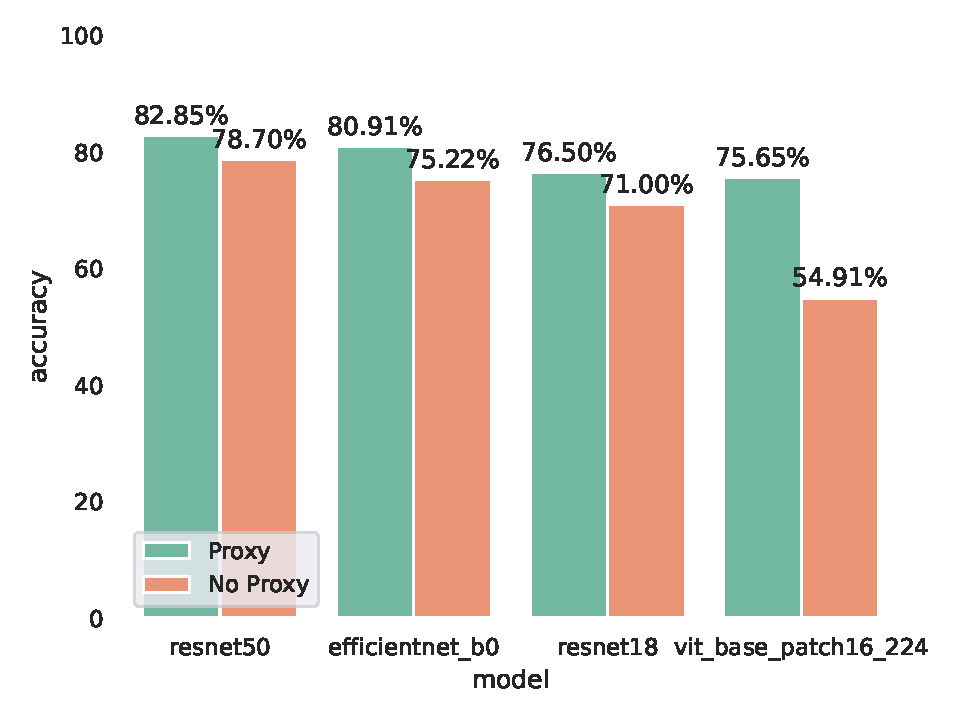
\includegraphics[width=1\textwidth]{results/cifar100_results.pdf}
    \caption{Comparing Accuracies of models trained with and without Proxy Attention on the Cifar100 dataset}
    \label{fig:cifar100_results}
\end{figure}

\subsection{Caltech101 Results}
This section shows the accuracies per model for the Caltech101 dataset. The results are shown in Figure \ref{fig:caltech101_results}. 
\begin{figure}[H]
    \centering
    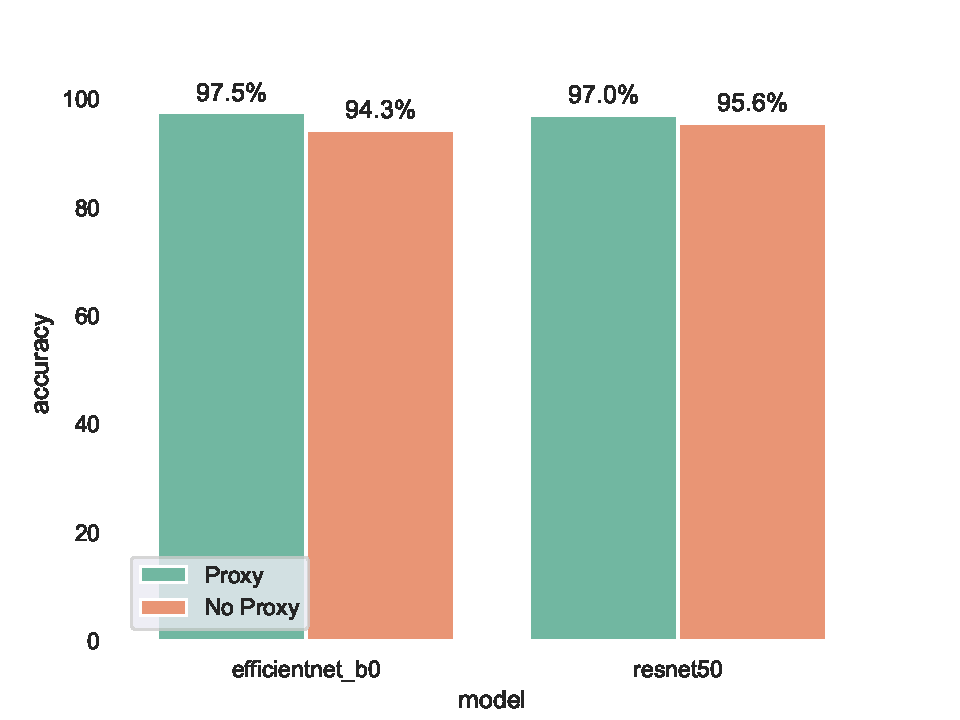
\includegraphics[width=1\textwidth]{results/caltech101_results.pdf}
    \caption{Comparing Accuracies of models trained with and without Proxy Attention on the Caltech101 dataset}
    \label{fig:caltech101_results}
\end{figure}

\subsection{Asl Results}
This section shows the accuracies per model for the Asl dataset. The results are shown in Figure \ref{fig:asl_results}. 
\begin{figure}[H]
    \centering
    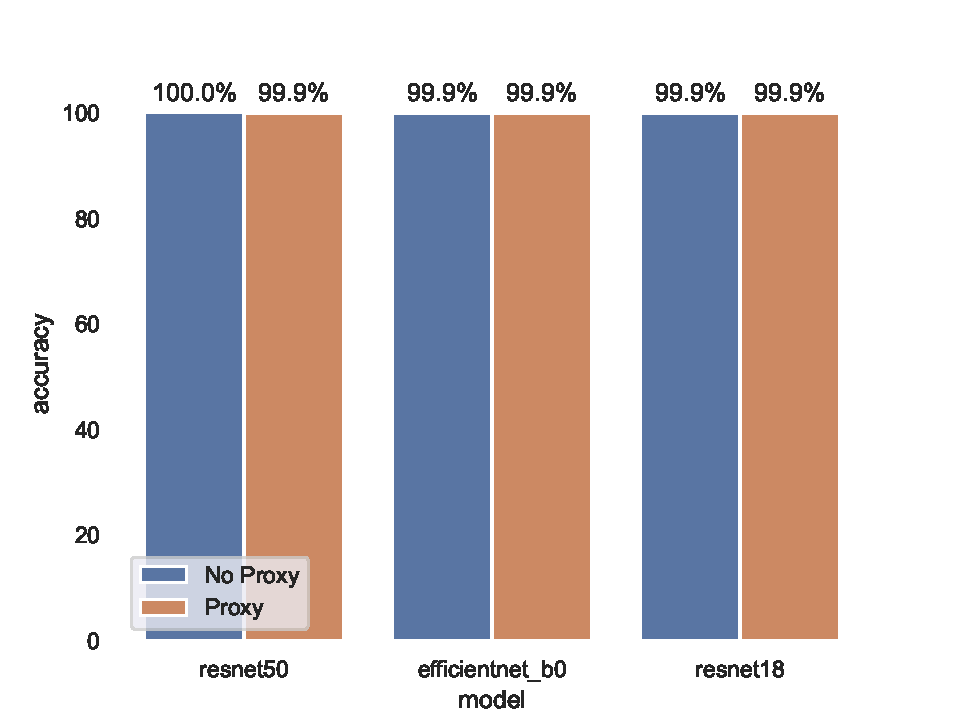
\includegraphics[width=1\textwidth]{results/asl_results.pdf}
    \caption{Comparing Accuracies of models trained with and without Proxy Attention on the Asl dataset}
    \label{fig:asl_results}
\end{figure}

\subsection{Plantdisease Results}
This section shows the accuracies per model for the Plantdisease dataset. The results are shown in Figure \ref{fig:plantdisease_results}. 
\begin{figure}[H]
    \centering
    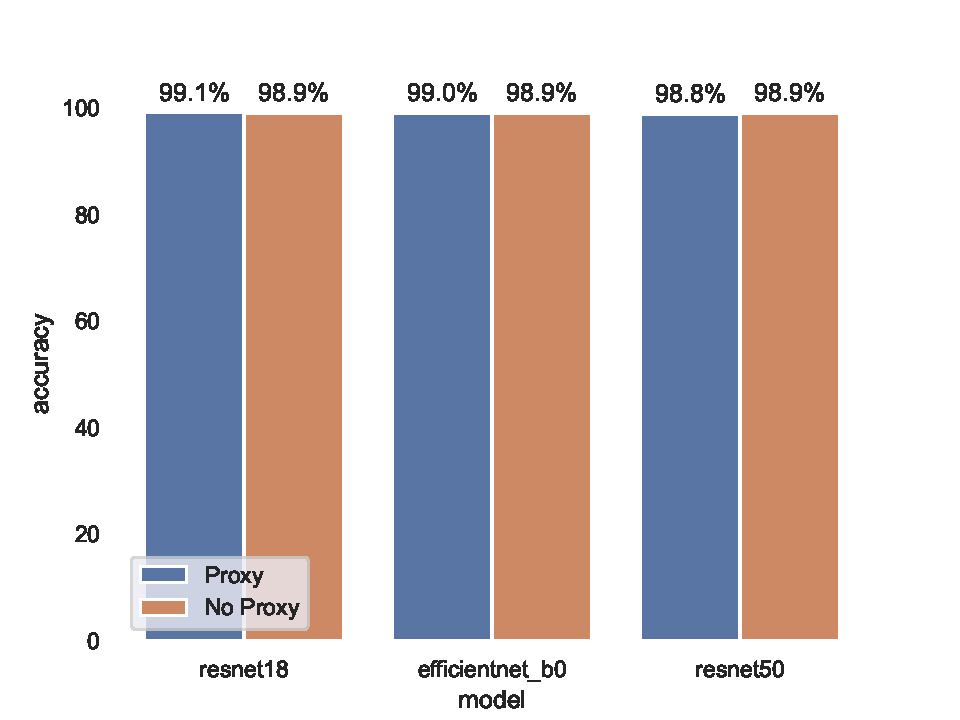
\includegraphics[width=1\textwidth]{results/plantdisease_results.pdf}
    \caption{Comparing Accuracies of models trained with and without Proxy Attention on the Plantdisease dataset}
    \label{fig:plantdisease_results}
\end{figure}


\subsection{Results Grouped By Schedule}
This section explores the validation accuracy obtained for different step schedules. The results are shown in Figure \ref{fig:schedresnet50_results}. 
\begin{figure}[H]
    \centering
    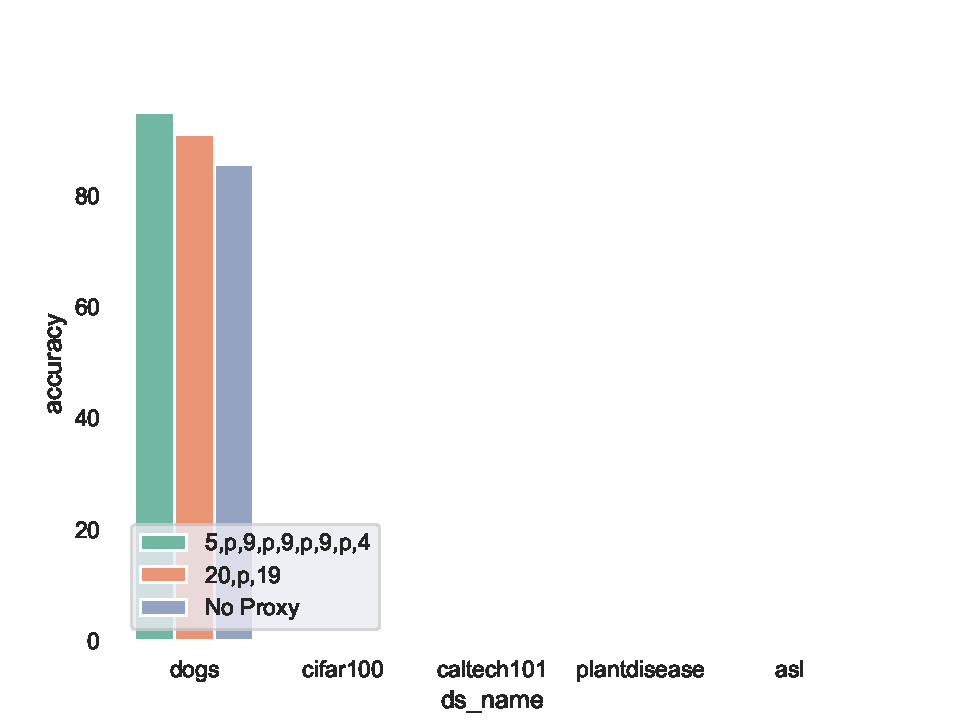
\includegraphics[width=1\textwidth]{results/schedule_resnet50.pdf}
    \caption{Comparing Accuracies of models trained with and without Proxy Attention on the ResNet50 \cite{heDeepResidualLearning2016} architecture for different step schedules}.
    \label{fig:schedresnet50_results}
\end{figure}

\subsection{Results Grouped By Proxy Threshold}
This section explores the validation accuracy obtained for different Proxy thresholds. The results are shown in Figure \ref{fig:proxy_threshold}. 
\begin{figure}[H]
    \centering
    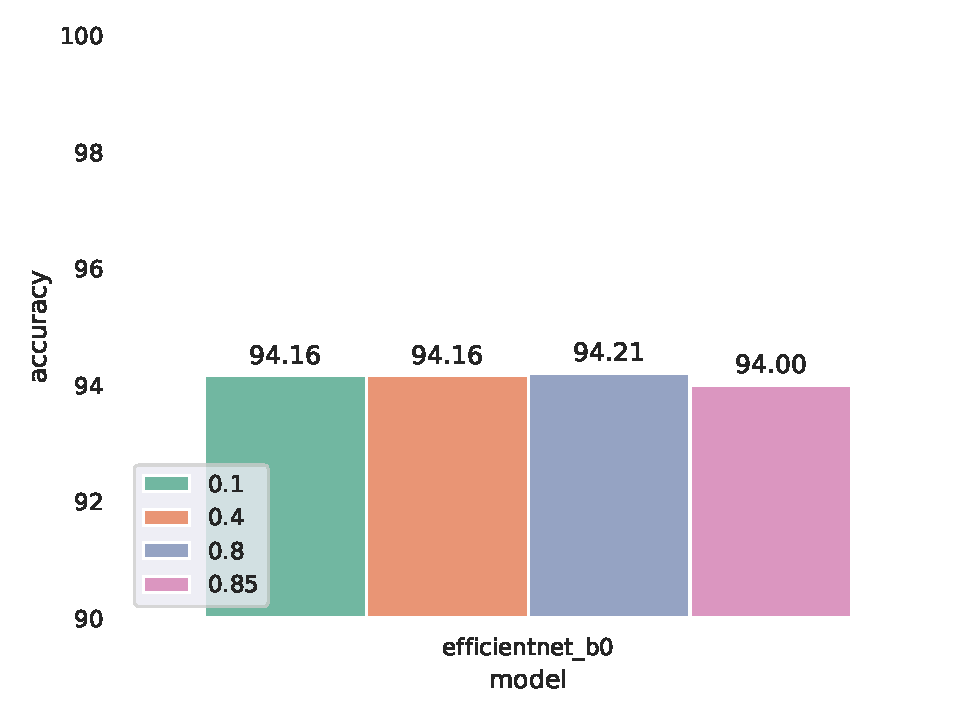
\includegraphics[width=1\textwidth]{results/proxy_threshold_results.pdf}
    \caption{Comparing Accuracies of EfficientNetB0 \cite{tanEfficientnetRethinkingModel2019} trained with Proxy Attention on the Stanford Dogs dataset\cite{khoslaNovelDatasetFineGrained} for different Proxy Thresholds}
    \label{fig:proxy_threshold}
\end{figure}

\begin{figure}[H]
    \centering
    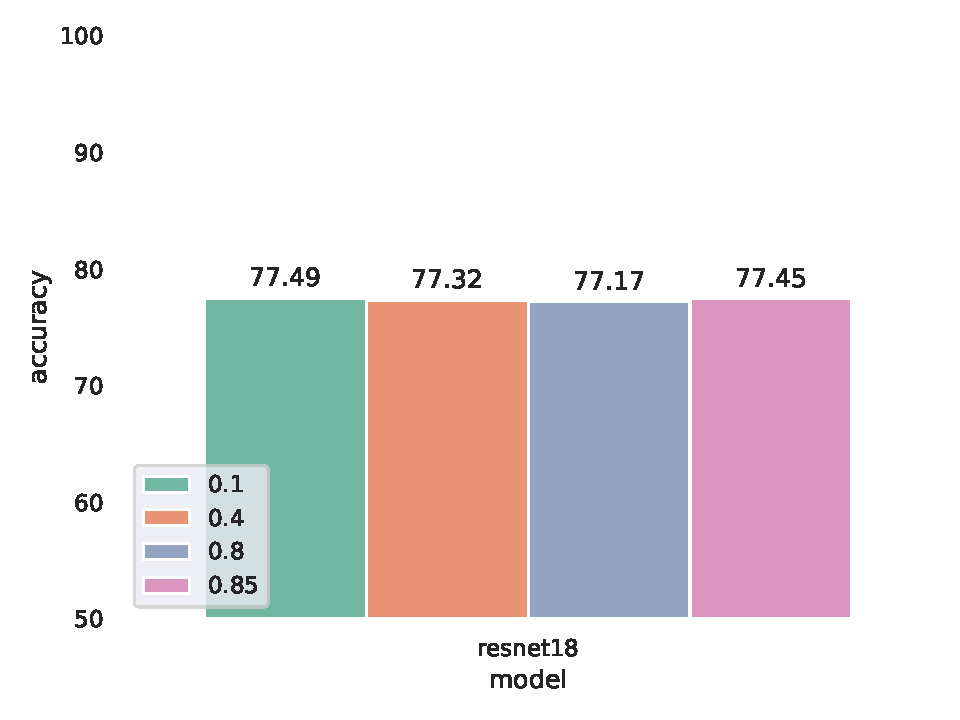
\includegraphics[width=1\textwidth]{results/proxy_threshold_results_tsing.pdf}
    \caption{Comparing Accuracies of Resnet18 \cite{heDeepResidualLearning2016} trained with Proxy Attention on the Tsinghua Dogs Dataset \cite{zouNewDatasetDog2020} for different Proxy Thresholds}
    \label{fig:proxy_threshold2}
\end{figure}

\subsection{Results Grouped By Proxy Image Weight}
This section explores the validation accuracy obtained for different Proxy image weights. The results are shown in Figure \ref{fig:proxy_weight}. 

\begin{figure}[H]
    \centering
    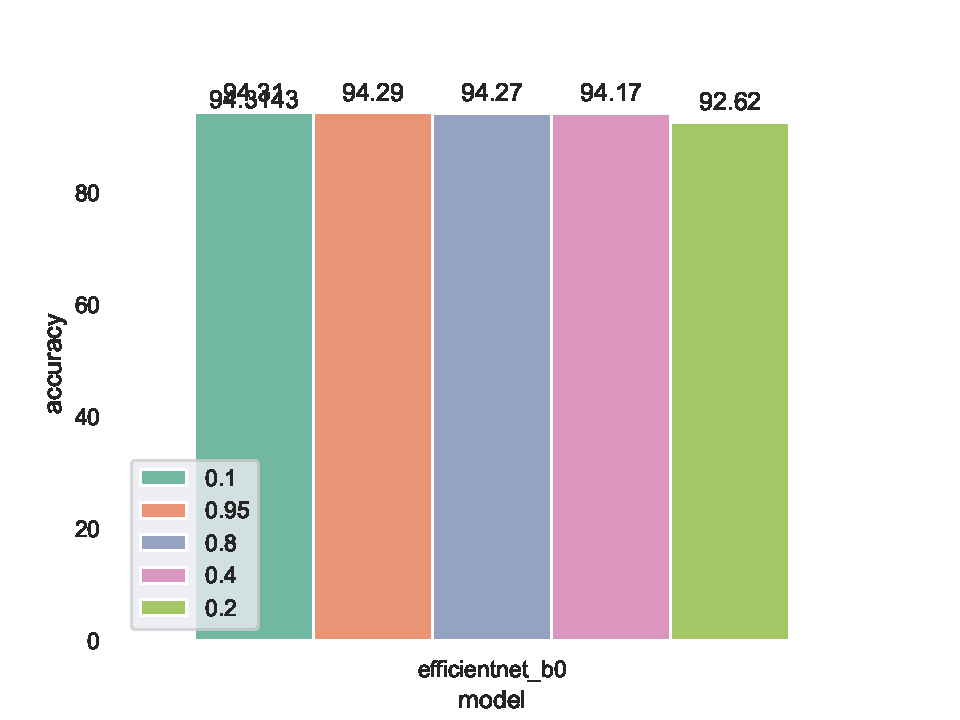
\includegraphics[width=1\textwidth]{results/proxy_weight_results.pdf}
    \caption{Comparing Accuracies of EfficientNetB0 \cite{tanEfficientnetRethinkingModel2019} trained with Proxy Attention on the Stanford Dogs dataset\cite{khoslaNovelDatasetFineGrained} for different Proxy Image Weights}
    \label{fig:proxy_weight}
\end{figure}

\begin{figure}[H]
    \centering
    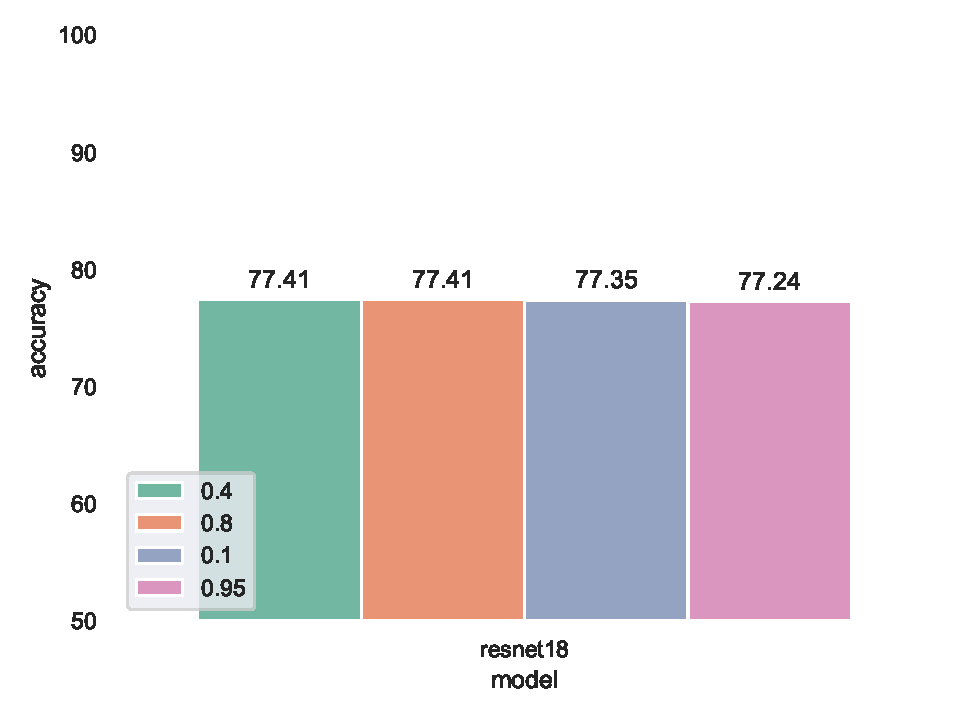
\includegraphics[width=1\textwidth]{results/proxy_weight_results_tsing.pdf}
    \caption{Comparing Accuracies of Resnet18 \cite{heDeepResidualLearning2016} trained with Proxy Attention on the Tsinghua Dogs Dataset \cite{zouNewDatasetDog2020} for different Proxy Image Weights}
    \label{fig:proxy_weight2}
\end{figure}

\subsection{Results Grouped By Proxy Image Subset}
This section explores the validation accuracy obtained for different Proxy image subsets. The results are shown in Figure \ref{fig:proxy_subset}.

\begin{figure}[H]
    \centering
    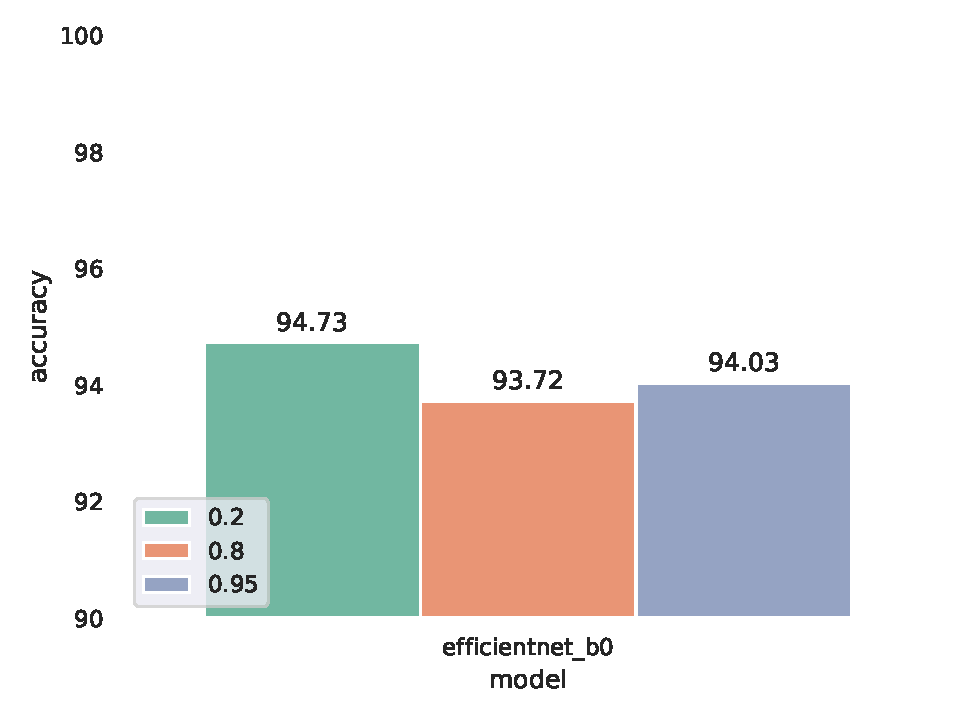
\includegraphics[width=1\textwidth]{results/proxy_subset_attention_results.pdf}
    \caption{Comparing Accuracies of EfficientNetB0 \cite{tanEfficientnetRethinkingModel2019} trained with Proxy Attention on the Stanford Dogs dataset\cite{khoslaNovelDatasetFineGrained} for different Proxy Image Subsets}
    \label{fig:proxy_subset}
\end{figure}

\begin{figure}[H]
    \centering
    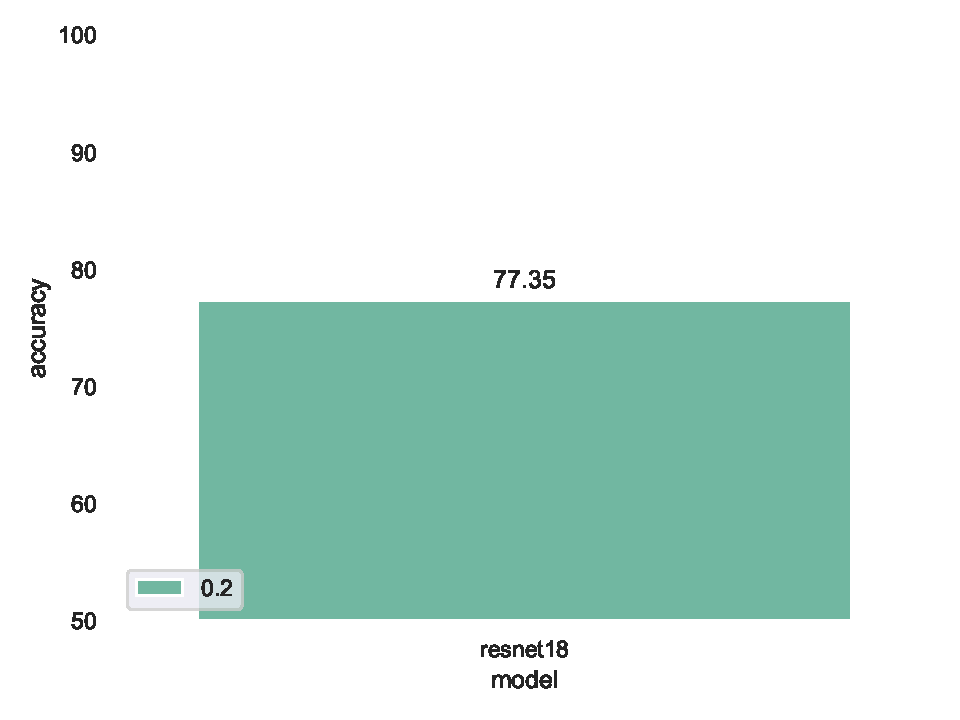
\includegraphics[width=1\textwidth]{results/proxy_subset_results_tsing.pdf}
    \caption{Comparing Accuracies of Resnet18 \cite{heDeepResidualLearning2016} trained with Proxy Attention on the Tsinghua Dogs Dataset \cite{zouNewDatasetDog2020} for different Proxy Image Subsets}
    \label{fig:proxy_subset2}
\end{figure}


\section{Explanability}
This section explores the explainability of the models for different hyperparameters and datasets by using a trained model to generate attention maps for a given input image. The attention maps are compared between the same network (with the same hyperparameters) trained with and without Proxy Attention.

\subsection{CIFAR 100, ResNet18, EigenGradCAM}

    \begin{figure}[H]
        \centering
        \begin{subfigure}[b]{1\textwidth}
            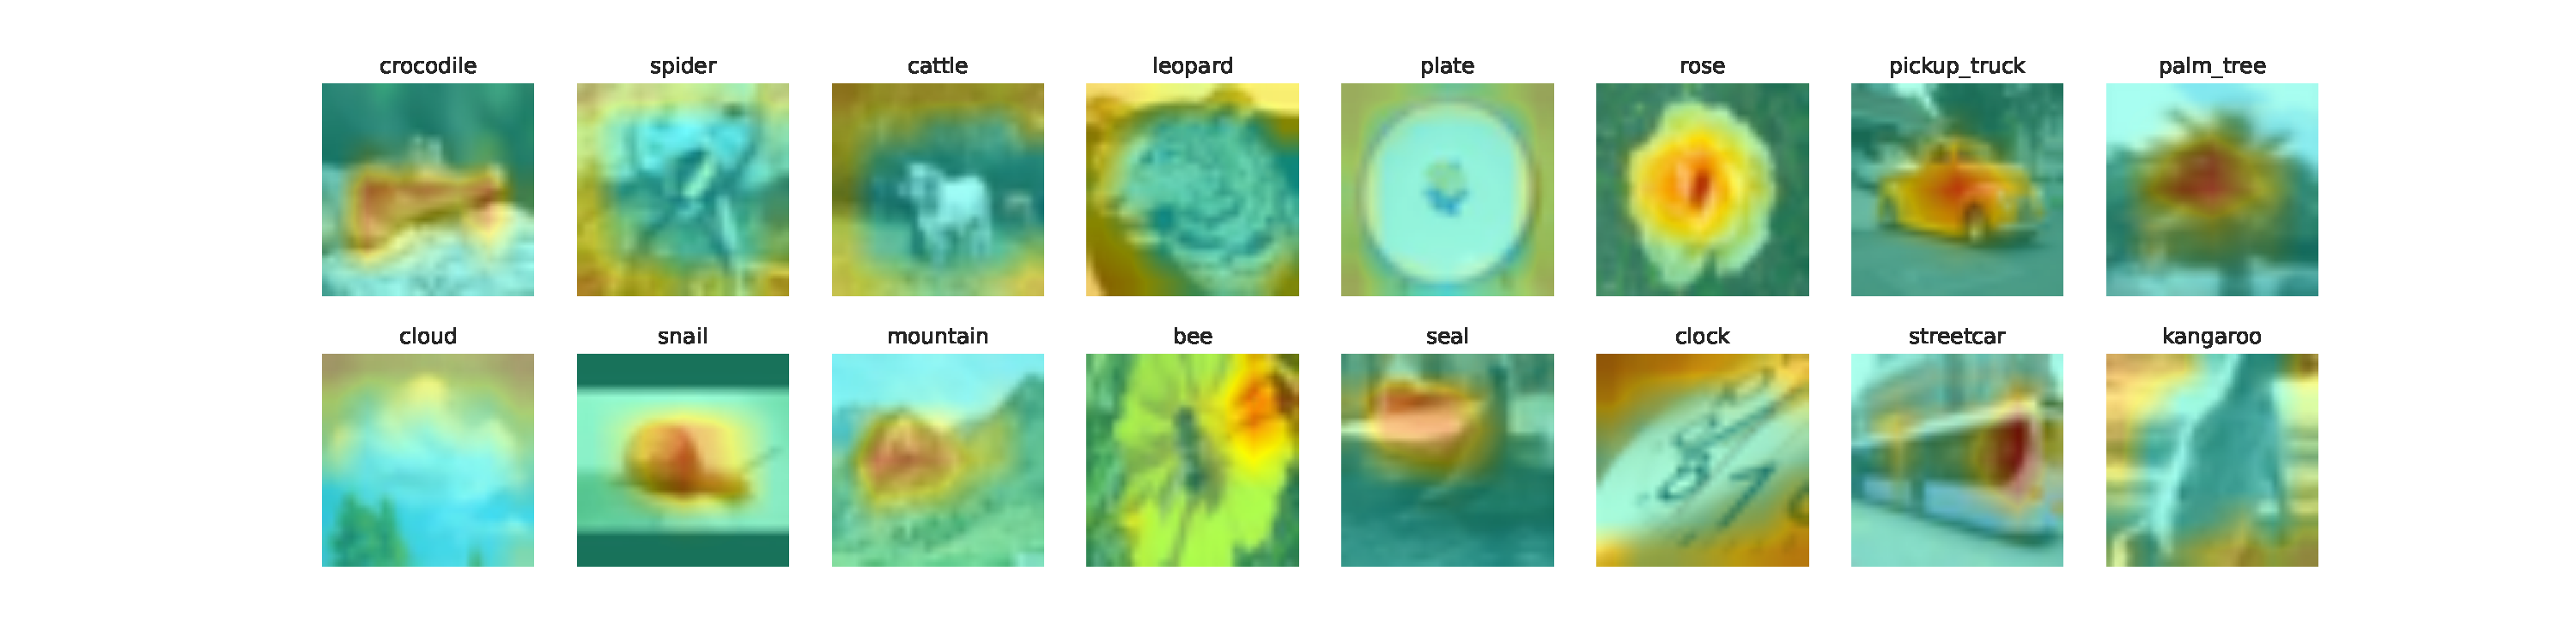
\includegraphics[width=\textwidth]{images/cifar100_resnet18_noproxy_0.pdf}
            \caption{Without Proxy Attention}
        \end{subfigure}
        \hfill
        \begin{subfigure}[b]{1\textwidth}
            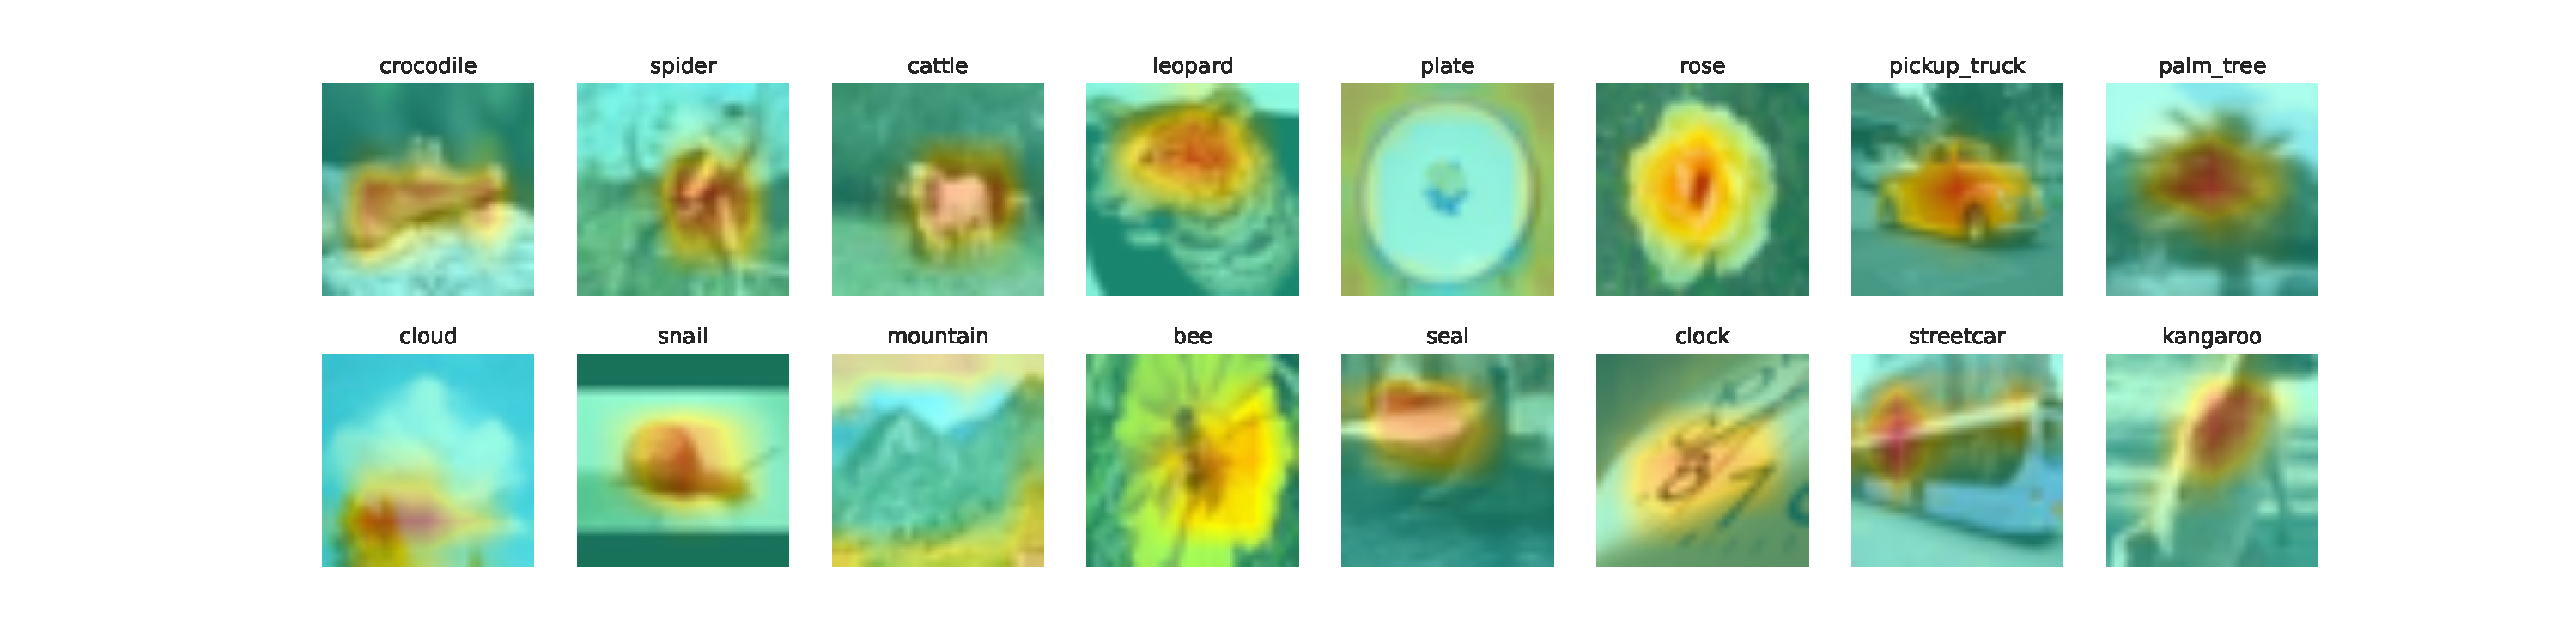
\includegraphics[width=\textwidth]{images/cifar100_resnet18_proxy_0.pdf}
            \caption{With Proxy Attention}
        \end{subfigure}
        \caption{Comparison of attention maps generated by resnet18 trained with and without Proxy Attention on the cifar100 dataset}
    \end{figure}
    

    \begin{figure}[H]
        \centering
        \begin{subfigure}[b]{1\textwidth}
            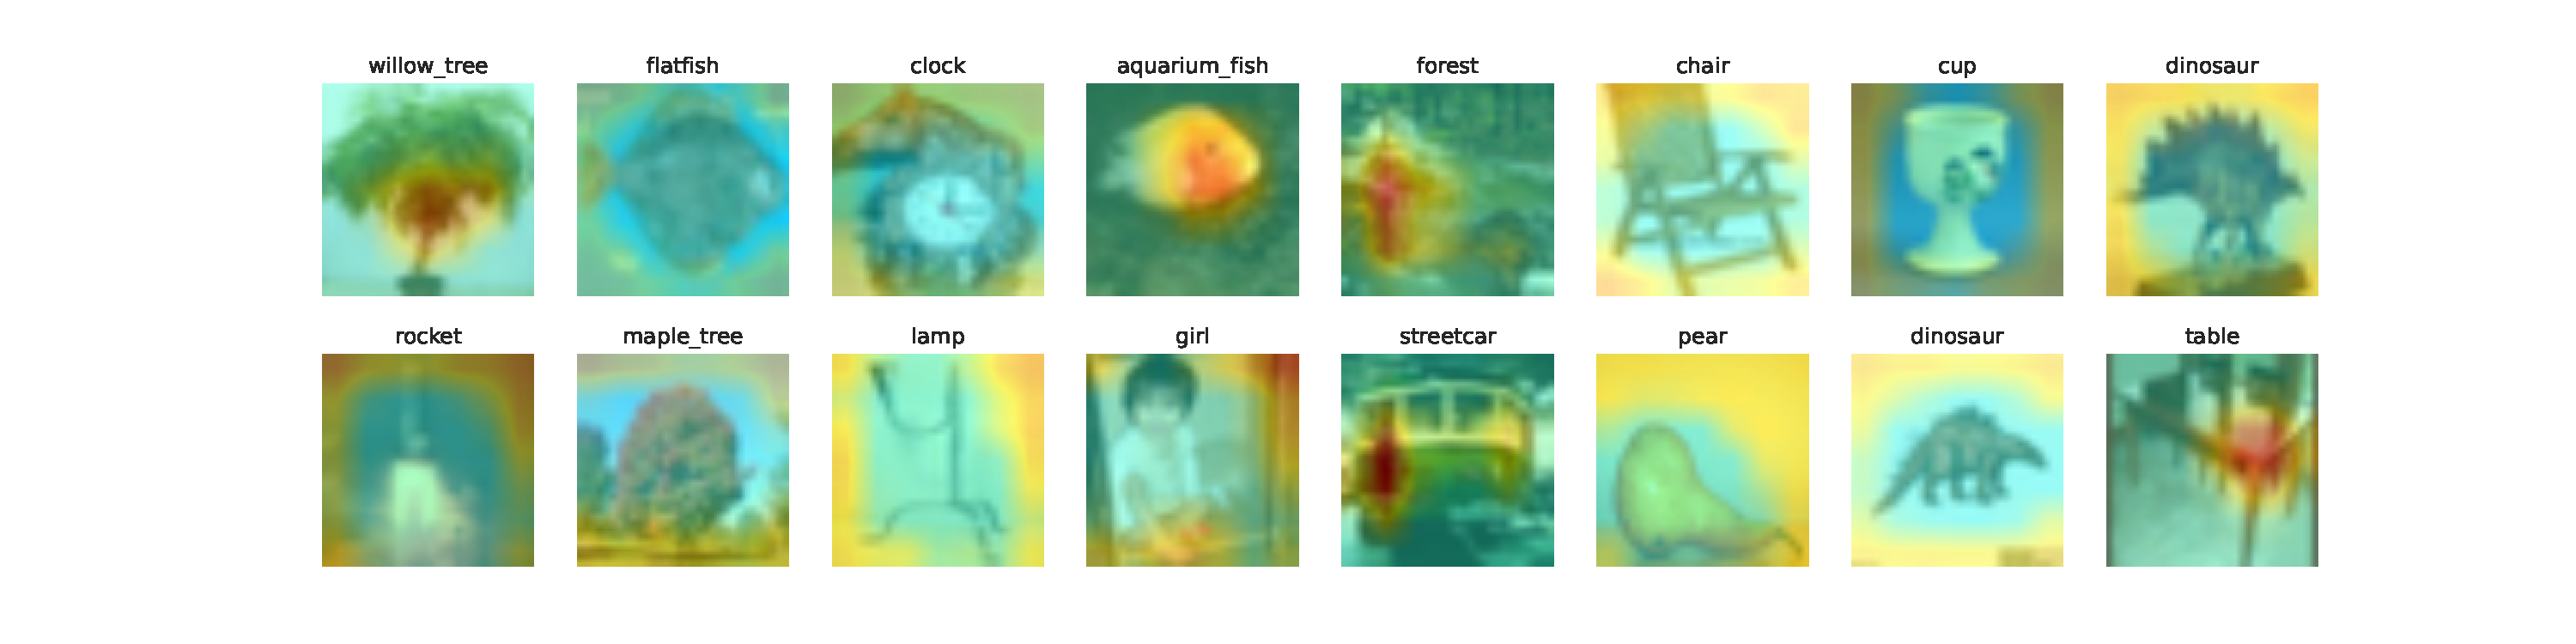
\includegraphics[width=\textwidth]{images/cifar100_resnet18_noproxy_1.pdf}
            \caption{Without Proxy Attention}
        \end{subfigure}
        \hfill
        \begin{subfigure}[b]{1\textwidth}
            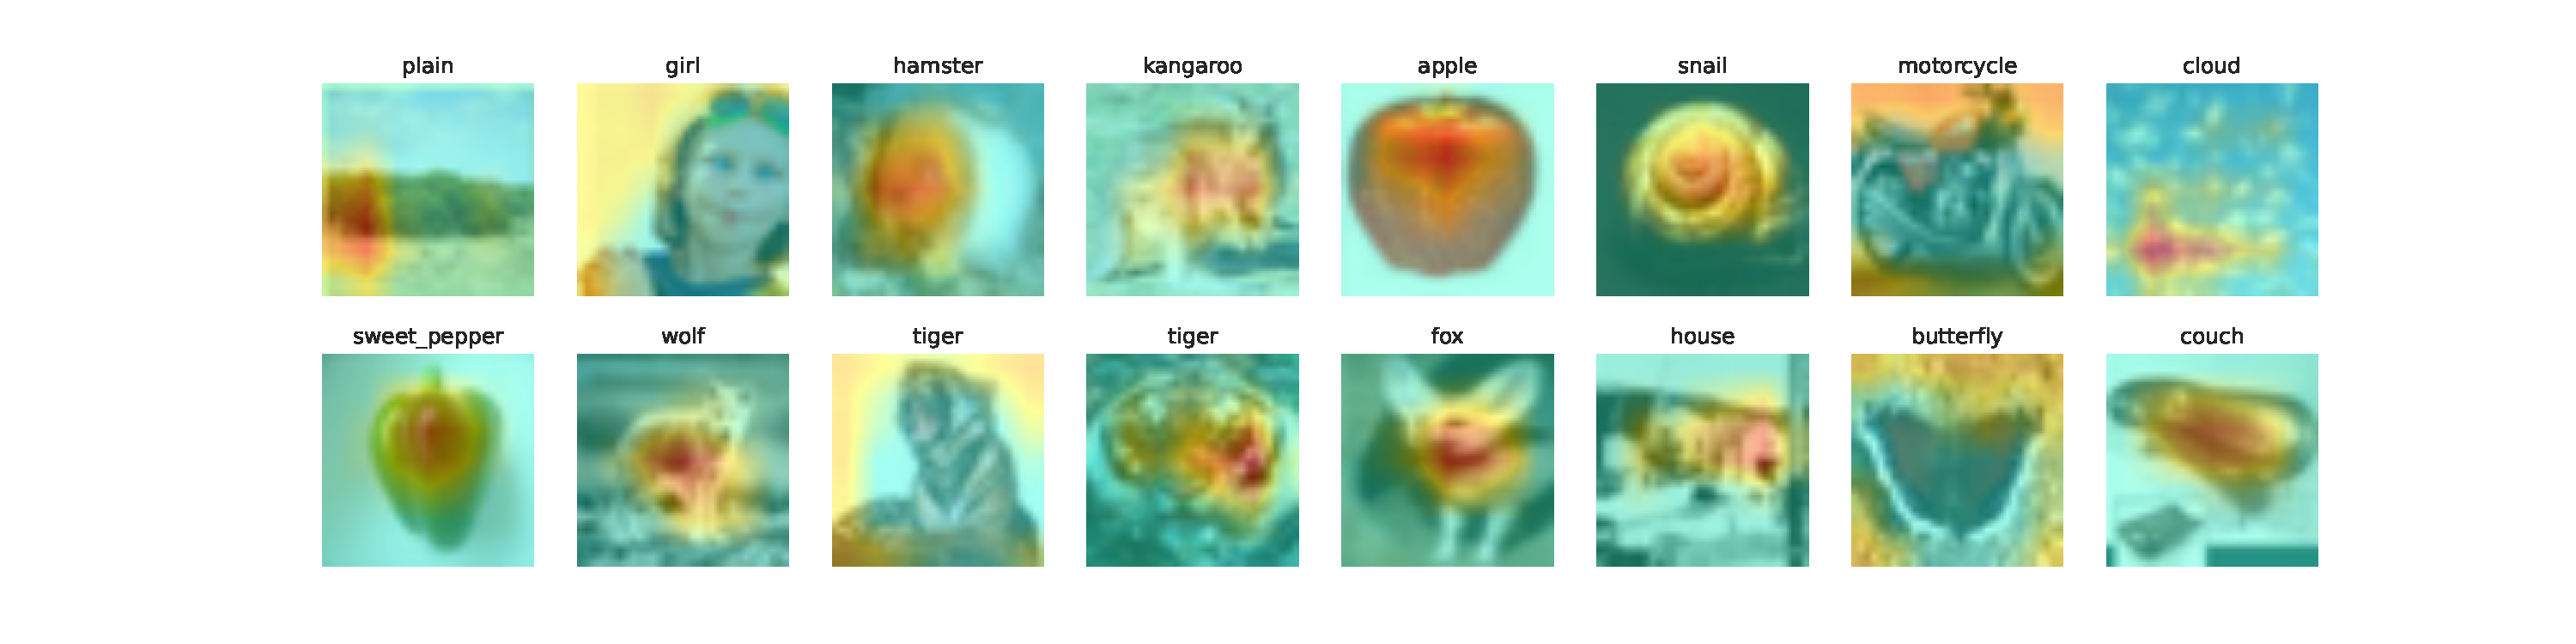
\includegraphics[width=\textwidth]{images/cifar100_resnet18_proxy_1.pdf}
            \caption{With Proxy Attention}
        \end{subfigure}
        \caption{Comparison of attention maps generated by resnet18 trained with and without Proxy Attention on the cifar100 dataset}
    \end{figure}
    

    \begin{figure}[H]
        \centering
        \begin{subfigure}[b]{1\textwidth}
            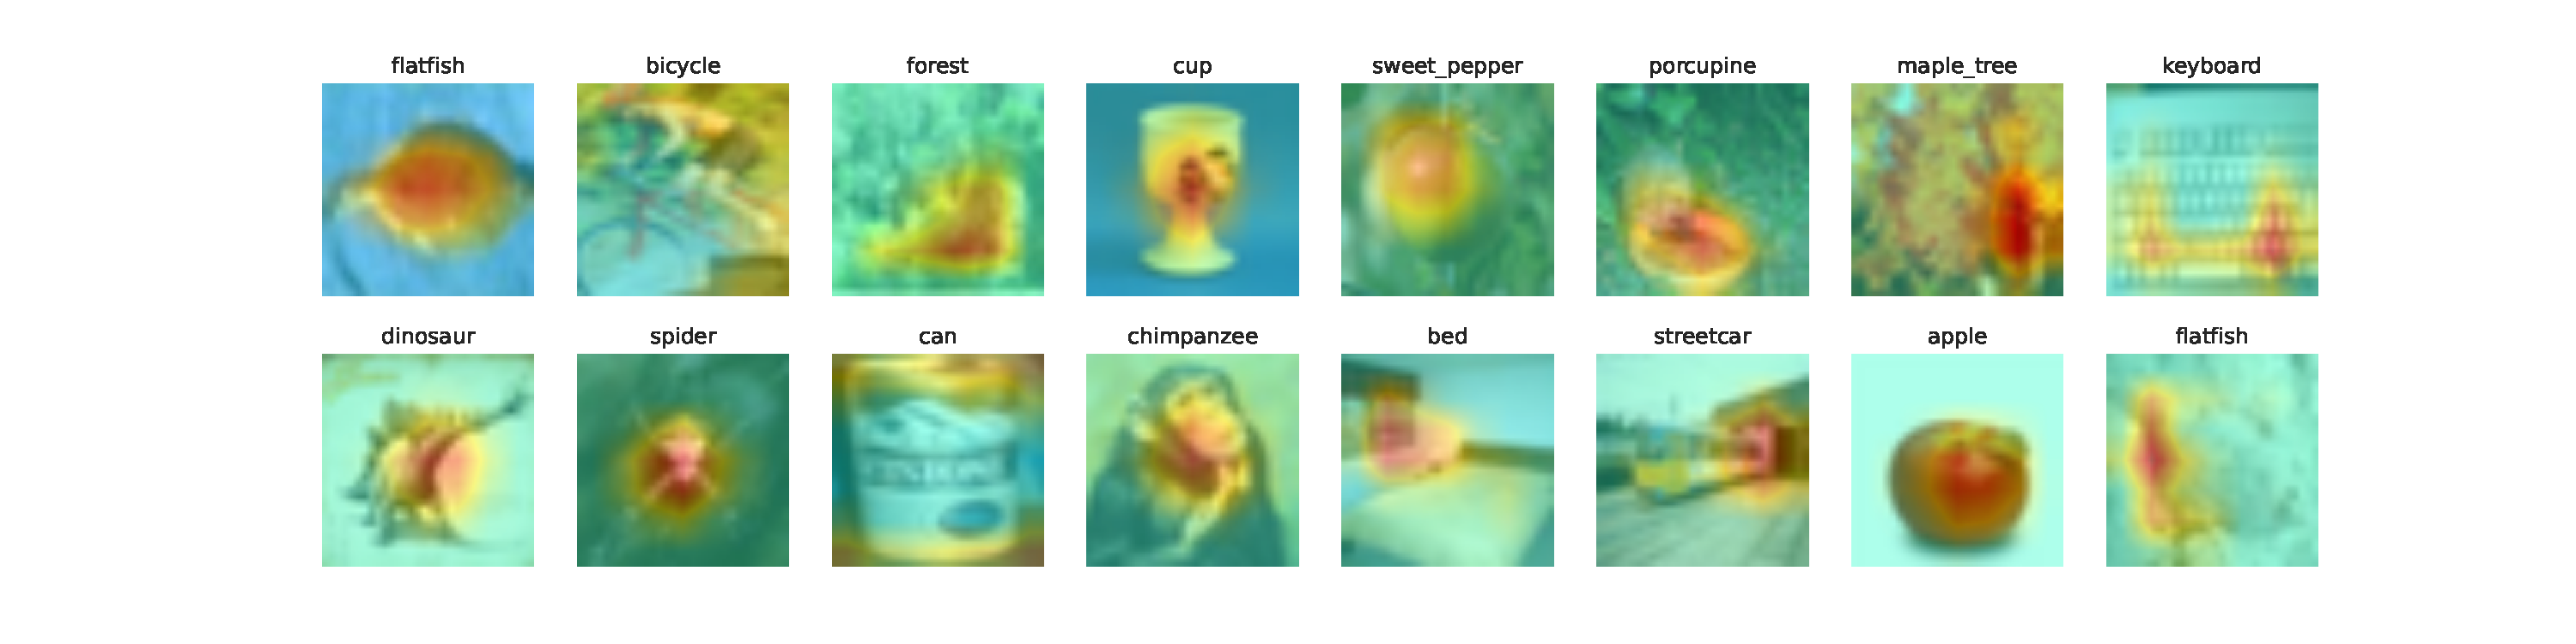
\includegraphics[width=\textwidth]{images/cifar100_resnet18_noproxy_2.pdf}
            \caption{Without Proxy Attention}
        \end{subfigure}
        \hfill
        \begin{subfigure}[b]{1\textwidth}
            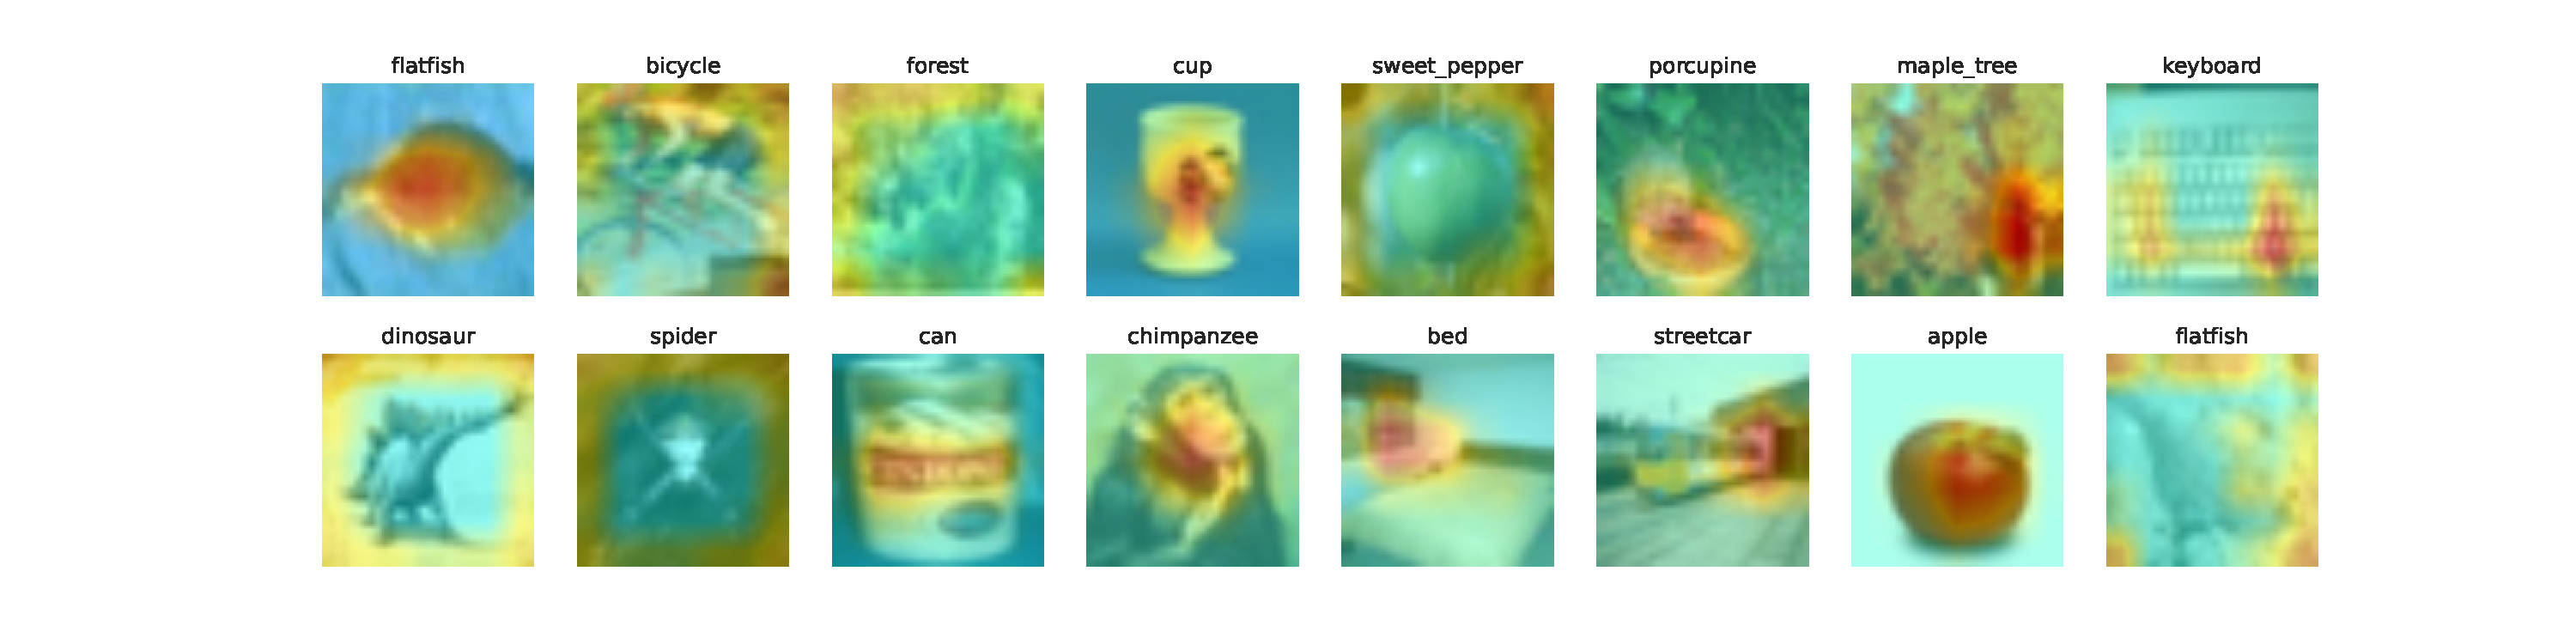
\includegraphics[width=\textwidth]{images/cifar100_resnet18_proxy_2.pdf}
            \caption{With Proxy Attention}
        \end{subfigure}
        \caption{Comparison of attention maps generated by resnet18 trained with and without Proxy Attention on the cifar100 dataset}
    \end{figure}
    

    \begin{figure}[H]
        \centering
        \begin{subfigure}[b]{1\textwidth}
            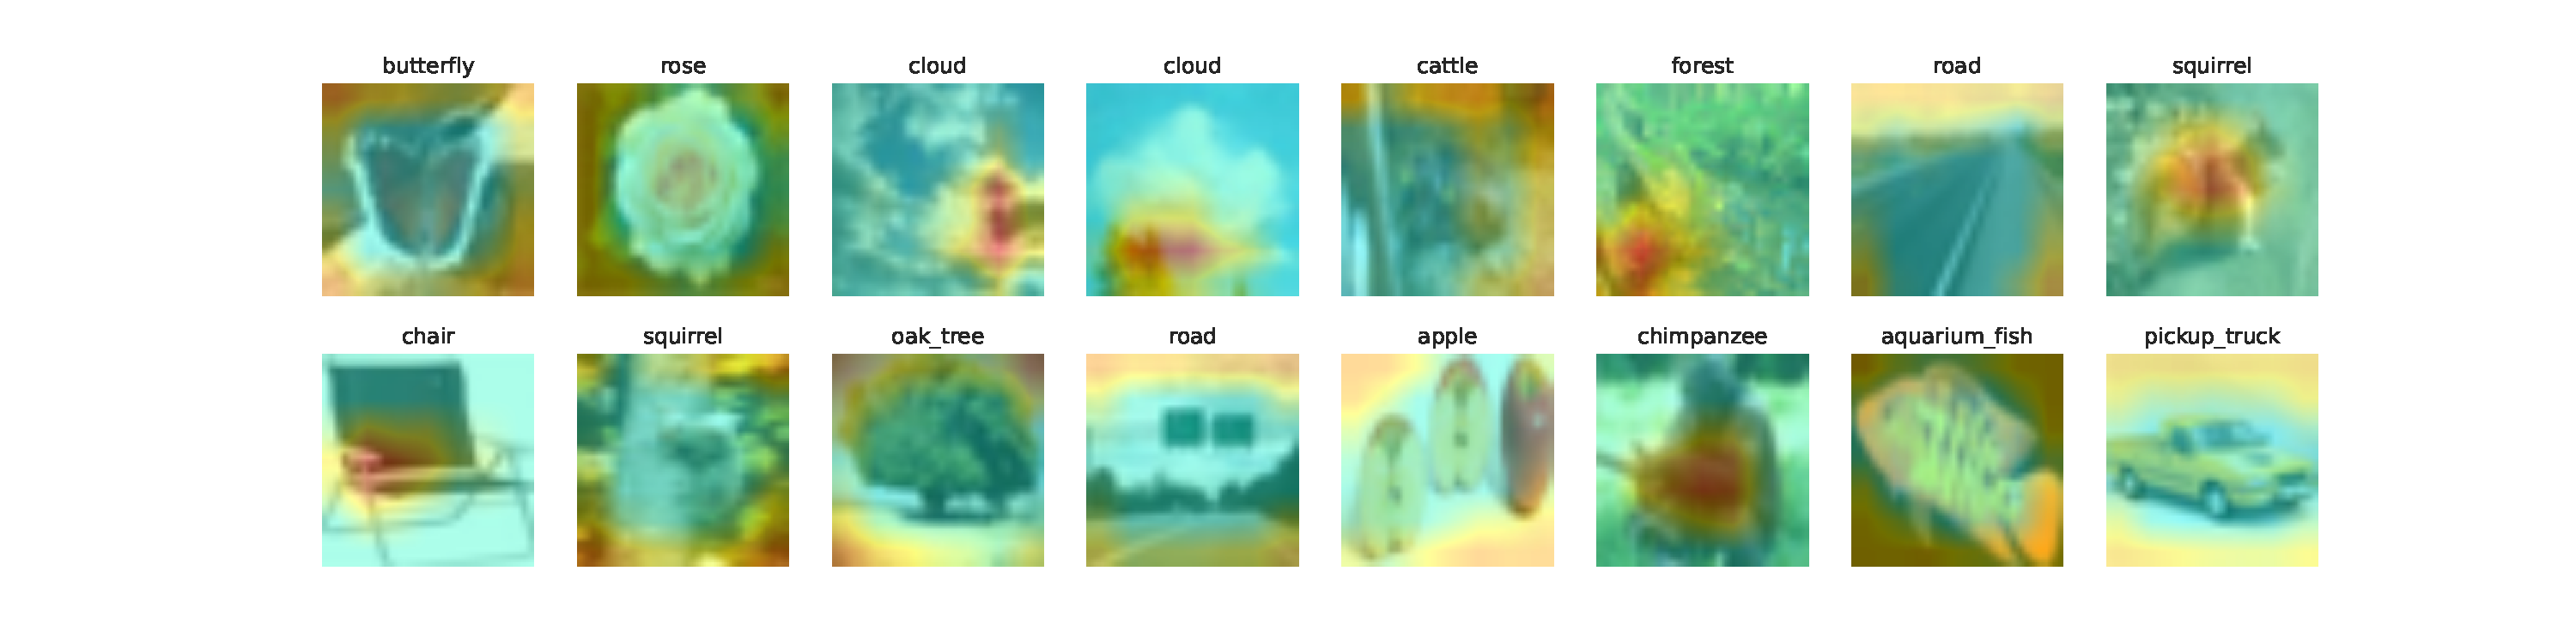
\includegraphics[width=\textwidth]{images/cifar100_resnet18_noproxy_3.pdf}
            \caption{Without Proxy Attention}
        \end{subfigure}
        \hfill
        \begin{subfigure}[b]{1\textwidth}
            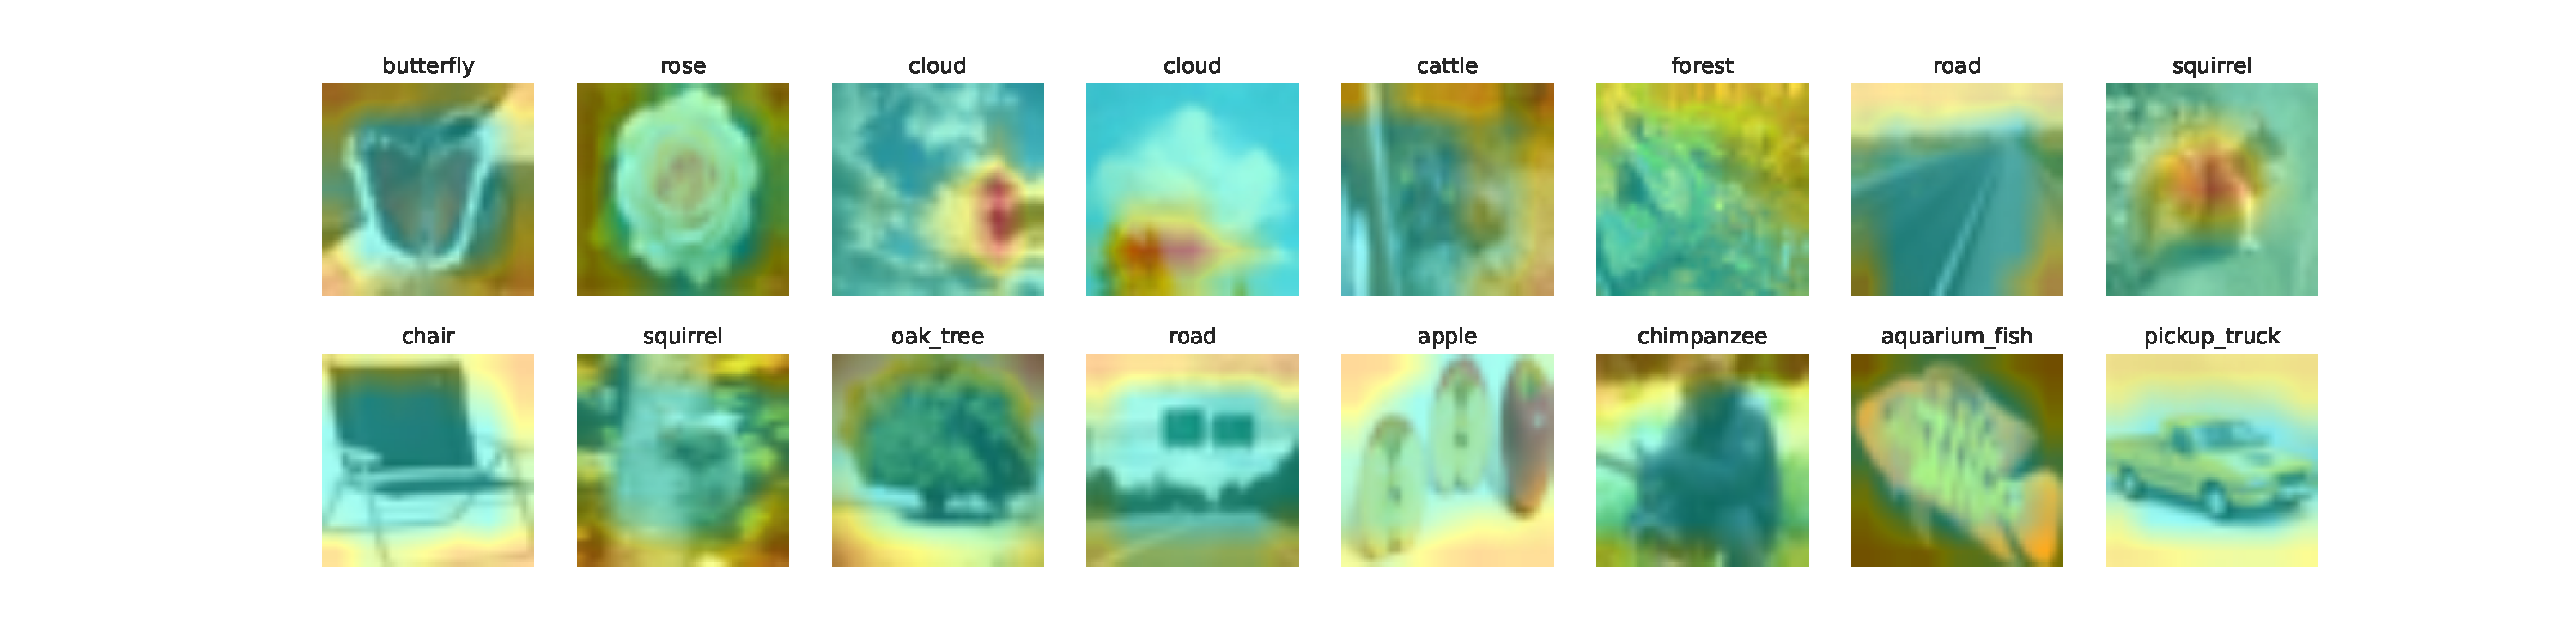
\includegraphics[width=\textwidth]{images/cifar100_resnet18_proxy_3.pdf}
            \caption{With Proxy Attention}
        \end{subfigure}
        \caption{Comparison of attention maps generated by resnet18 trained with and without Proxy Attention on the cifar100 dataset}
    \end{figure}
    


\subsection{CIFAR 100, EfficientNetB0, EigenGradCAM}

    \begin{figure}[H]
        \centering
        \begin{subfigure}[b]{1\textwidth}
            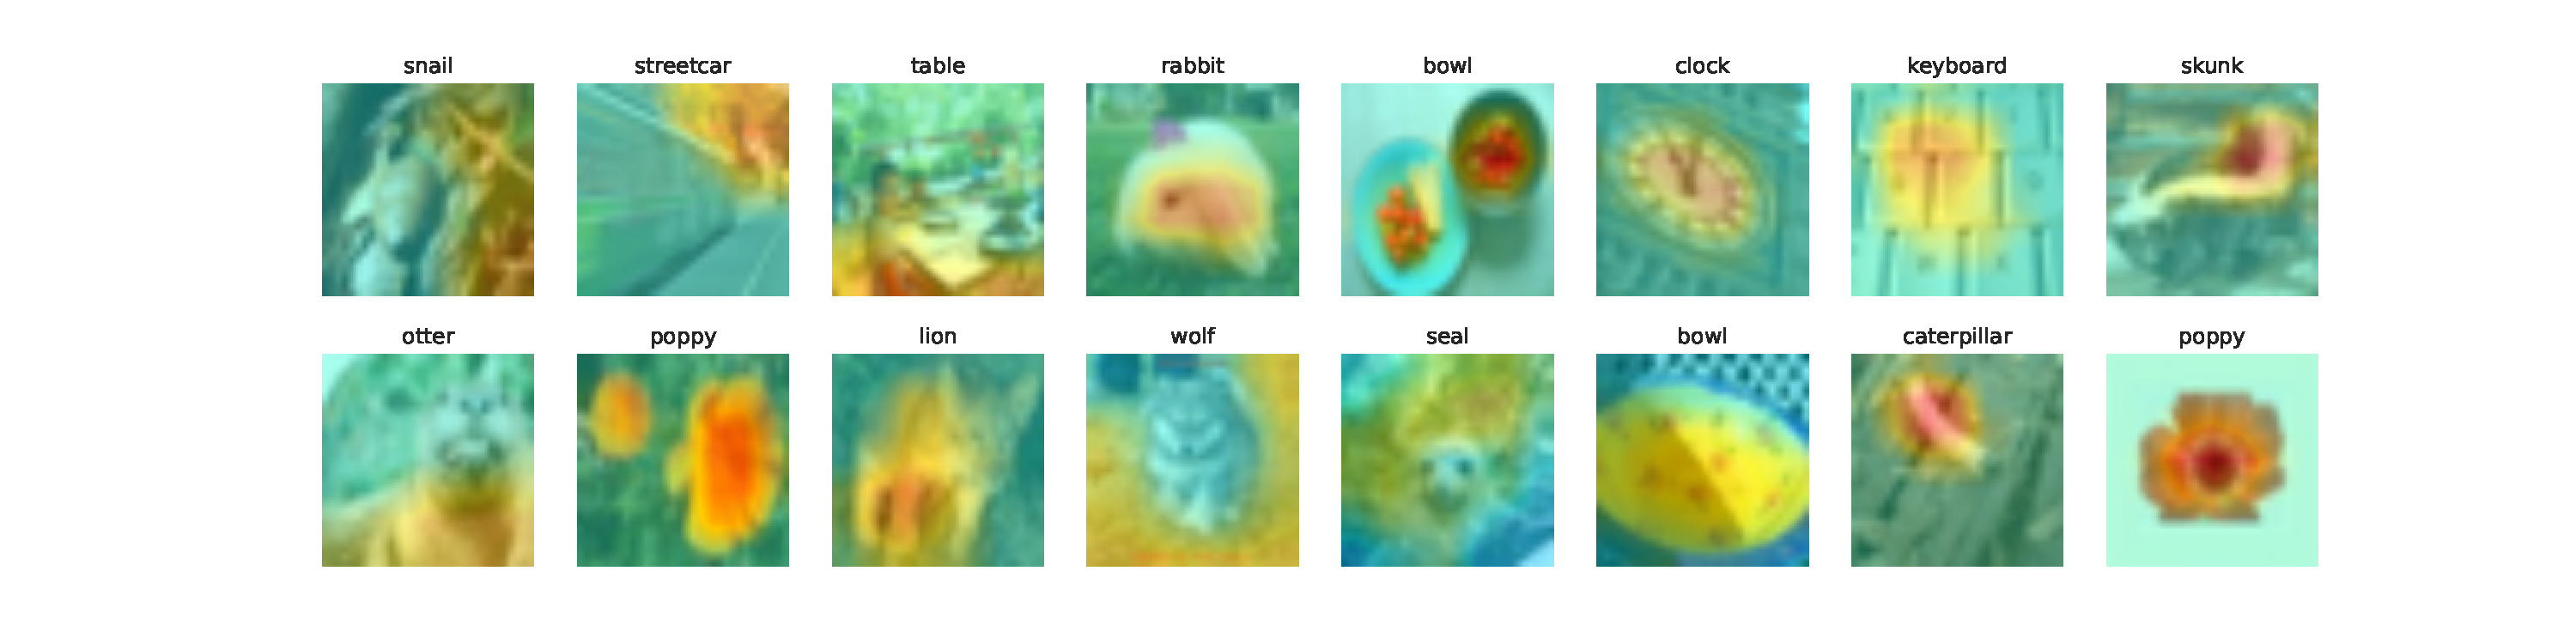
\includegraphics[width=\textwidth]{images/cifar100_efficientnet_b0_noproxy_0.pdf}
            \caption{Without Proxy Attention}
        \end{subfigure}
        \hfill
        \begin{subfigure}[b]{1\textwidth}
            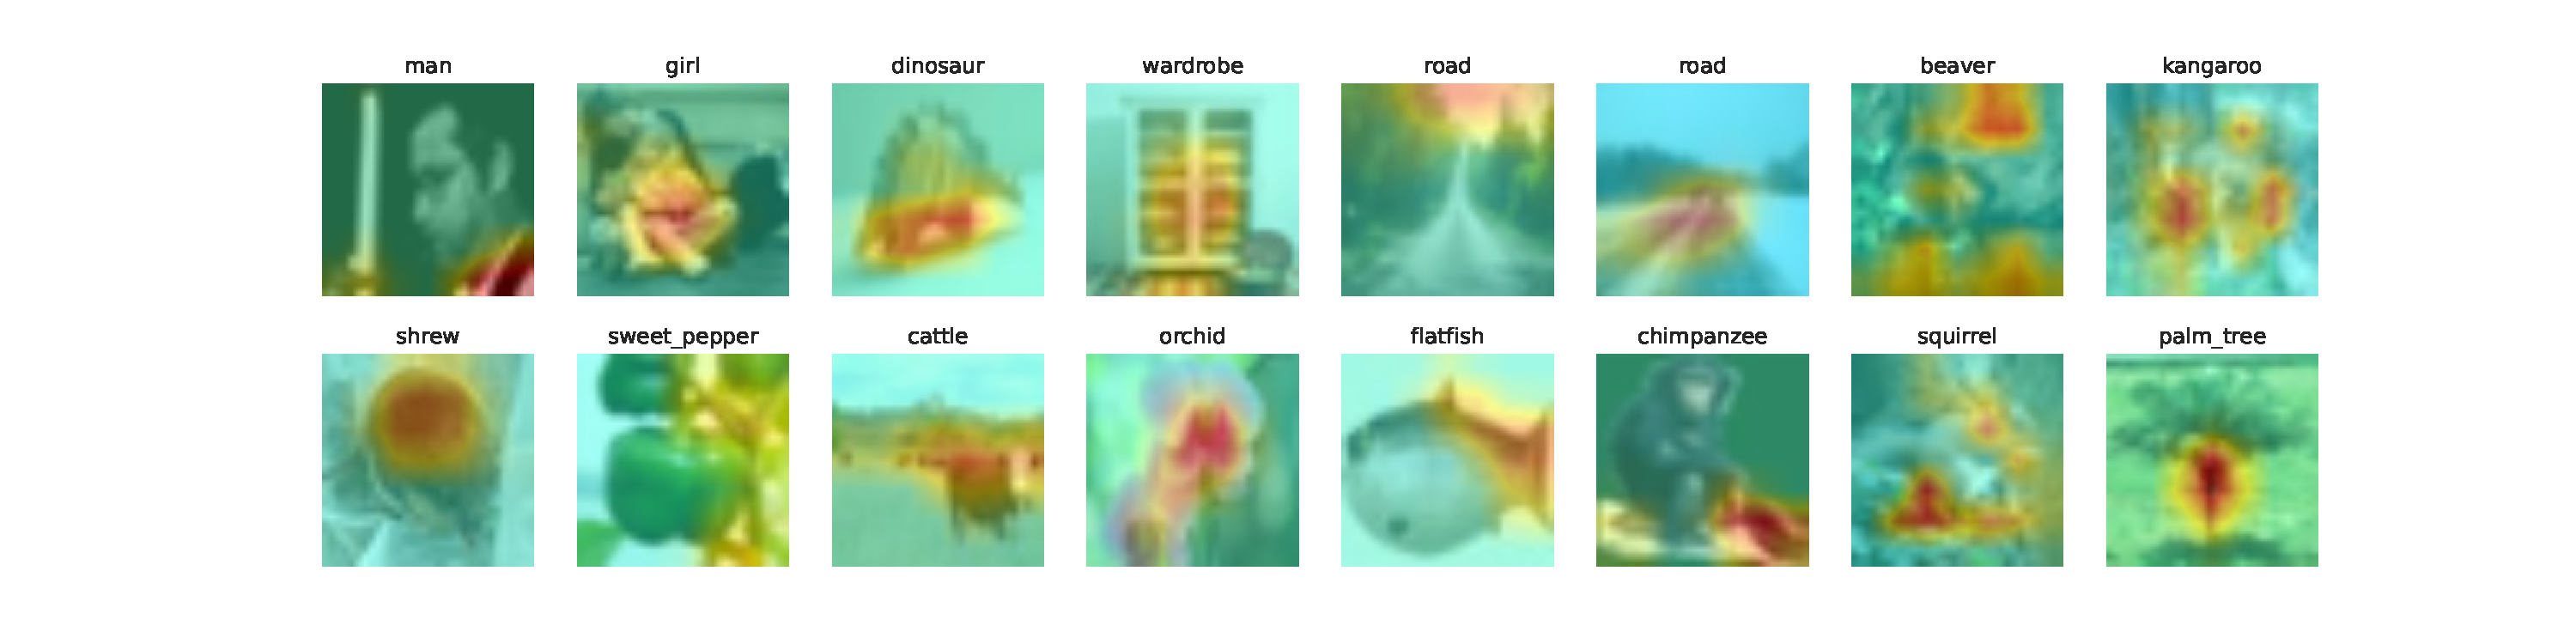
\includegraphics[width=\textwidth]{images/cifar100_efficientnet_b0_proxy_0.pdf}
            \caption{With Proxy Attention}
        \end{subfigure}
        \caption{Comparison of attention maps generated by efficientnet\_b0 trained with and without Proxy Attention on the cifar100 dataset}
    \end{figure}
    

    \begin{figure}[H]
        \centering
        \begin{subfigure}[b]{1\textwidth}
            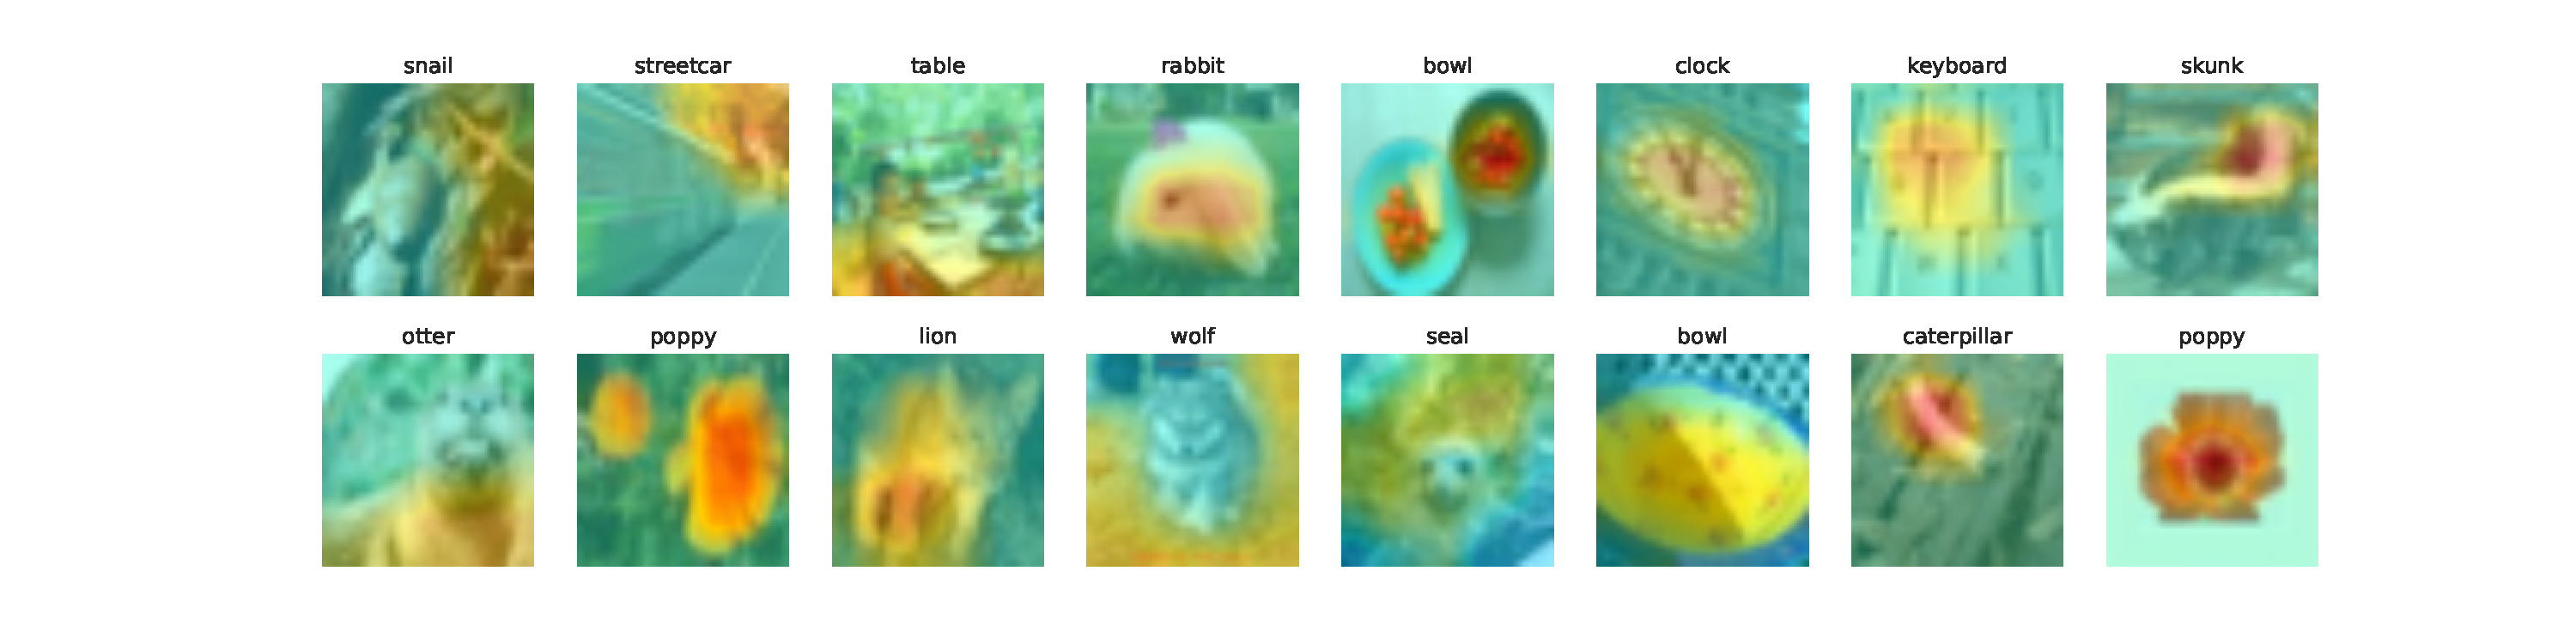
\includegraphics[width=\textwidth]{images/cifar100_efficientnet_b0_noproxy_0.pdf}
            \caption{Without Proxy Attention}
        \end{subfigure}
        \hfill
        \begin{subfigure}[b]{1\textwidth}
            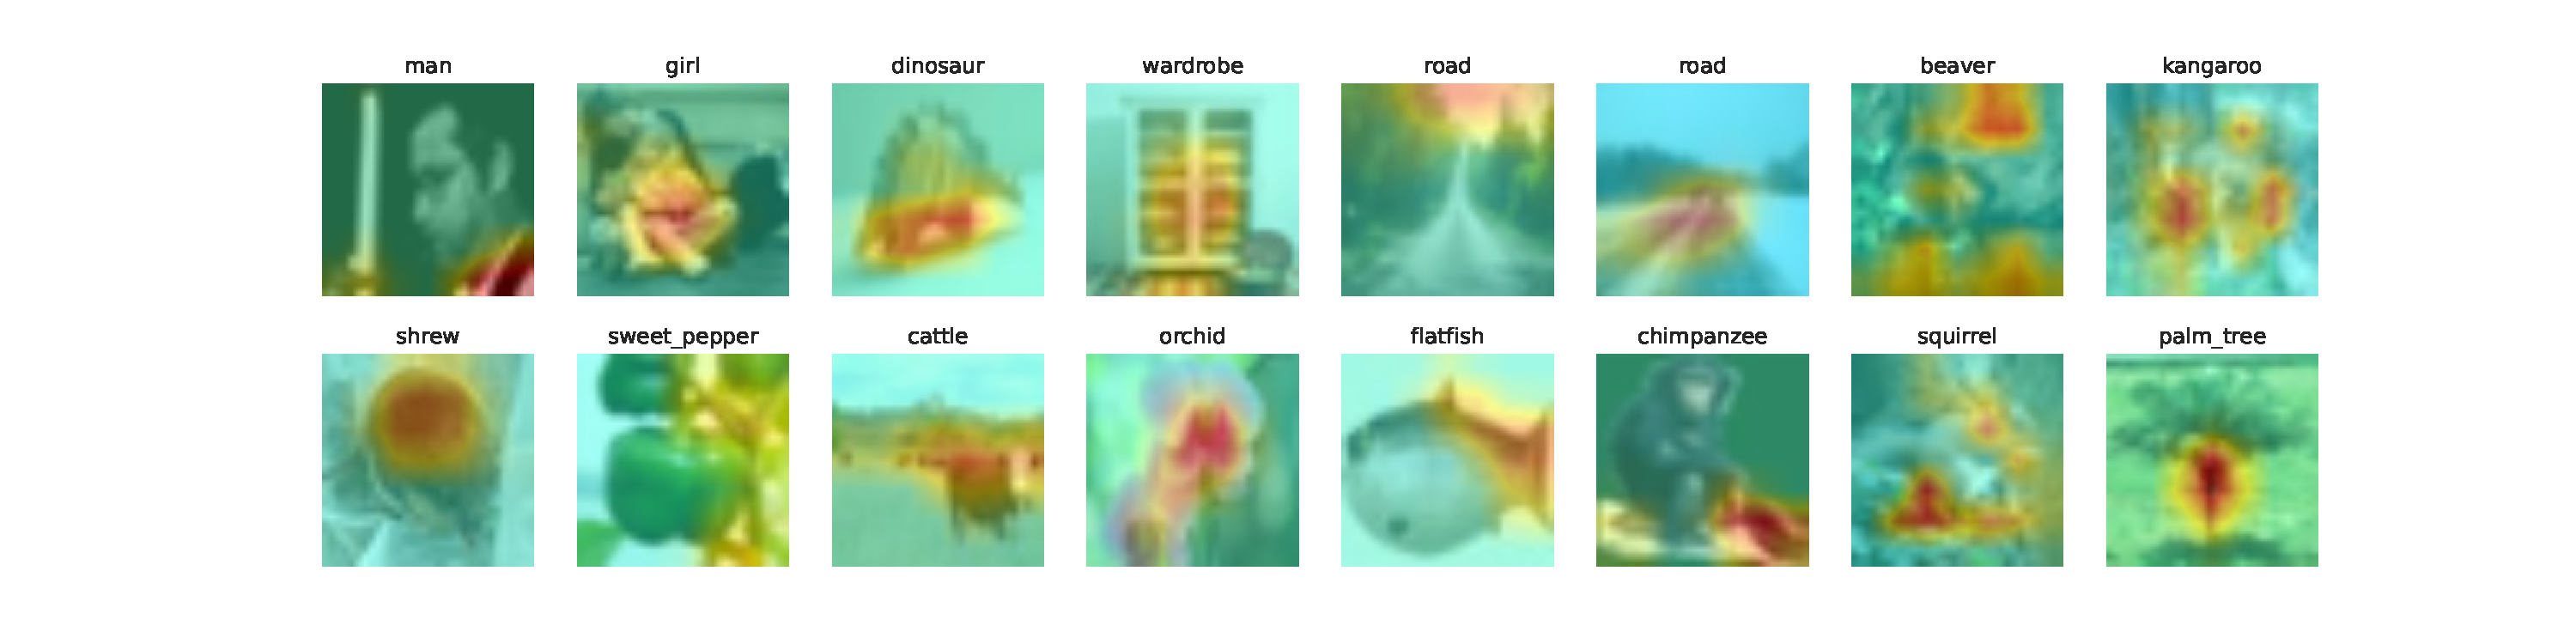
\includegraphics[width=\textwidth]{images/cifar100_efficientnet_b0_proxy_0.pdf}
            \caption{With Proxy Attention}
        \end{subfigure}
        \caption{Comparison of attention maps generated by efficientnet\_b0 trained with and without Proxy Attention on the cifar100 dataset}
    \end{figure}
    

    \begin{figure}[H]
        \centering
        \begin{subfigure}[b]{1\textwidth}
            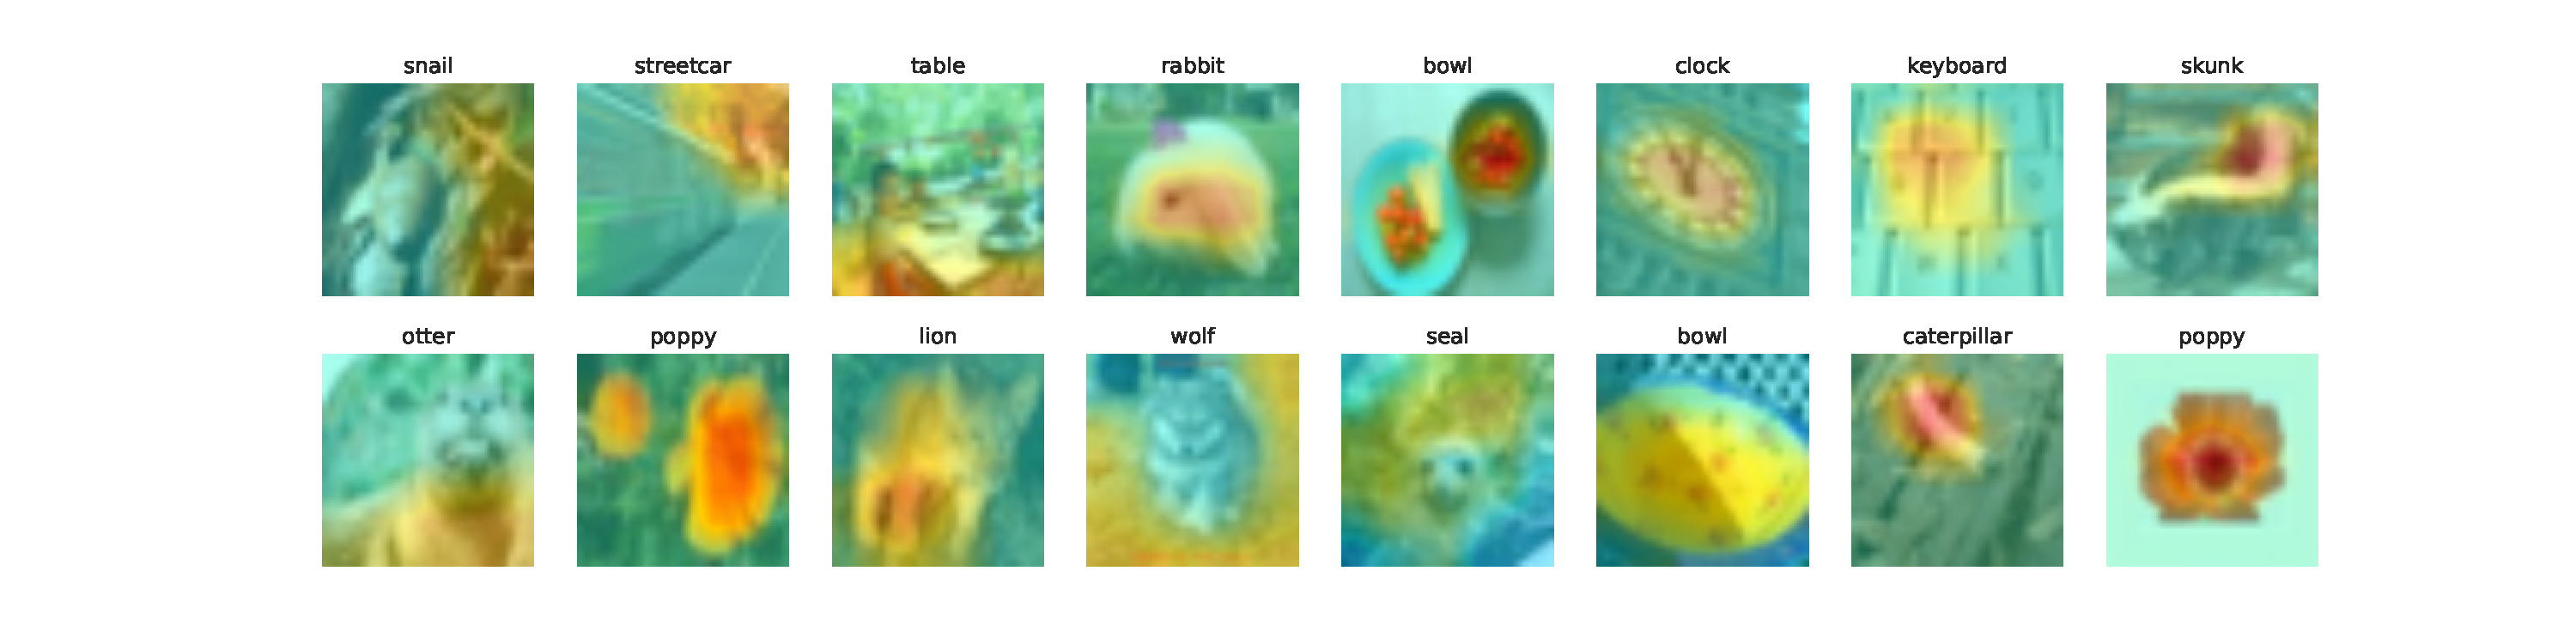
\includegraphics[width=\textwidth]{images/cifar100_efficientnet_b0_noproxy_0.pdf}
            \caption{Without Proxy Attention}
        \end{subfigure}
        \hfill
        \begin{subfigure}[b]{1\textwidth}
            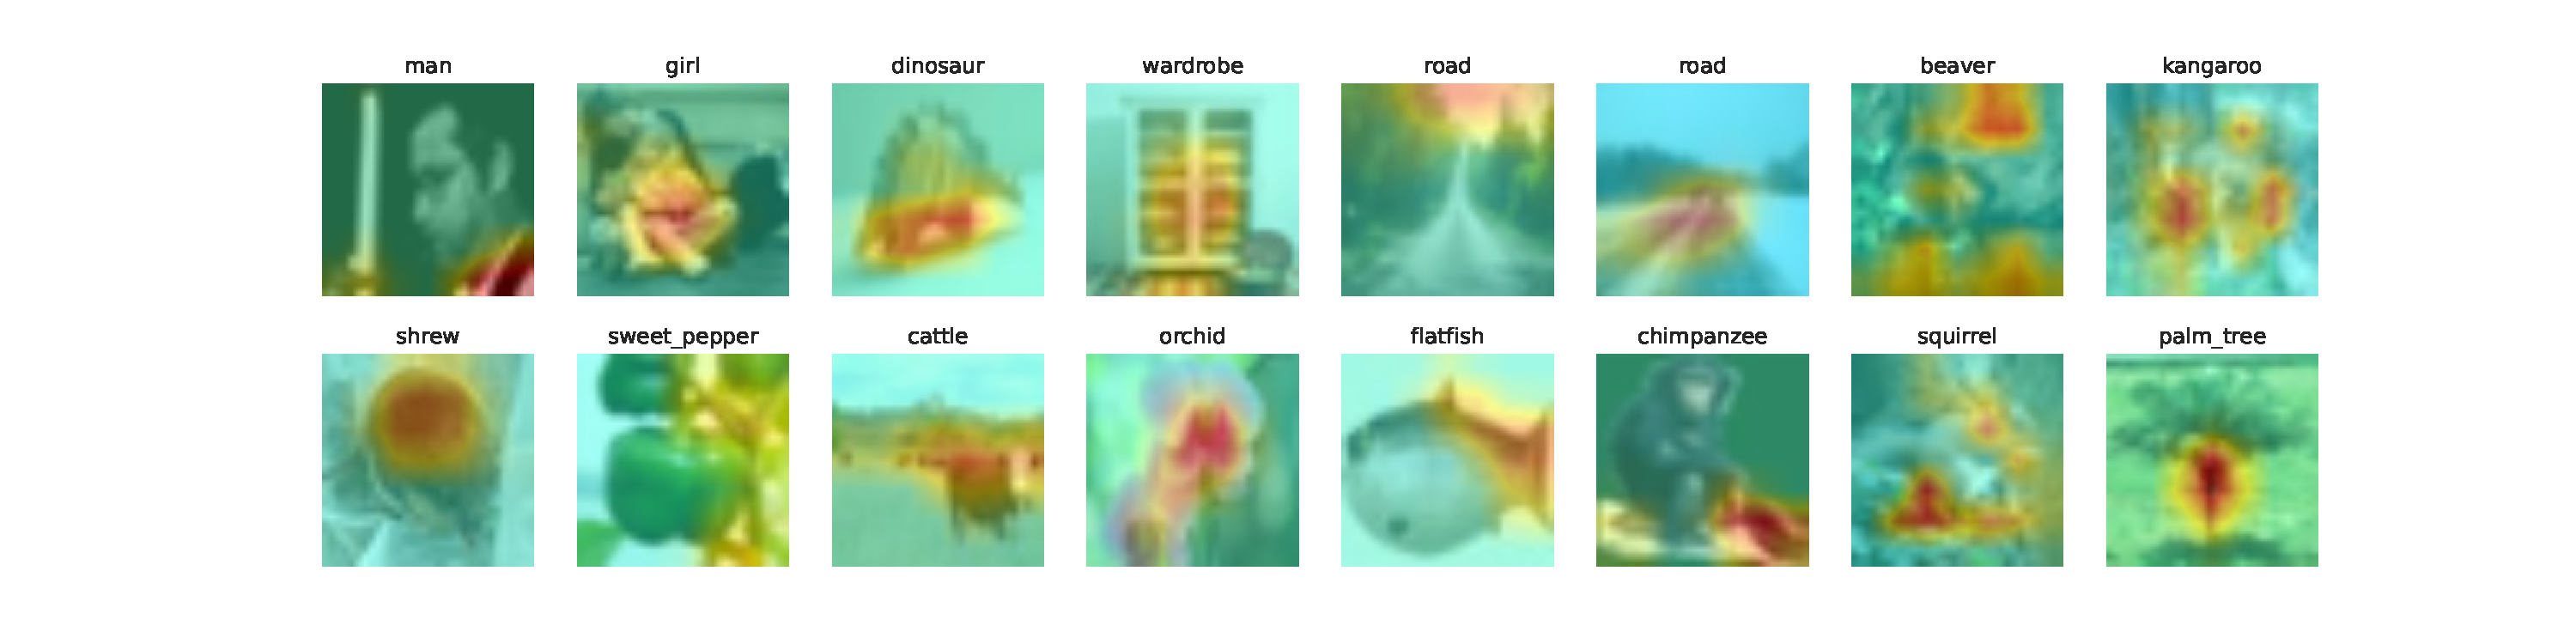
\includegraphics[width=\textwidth]{images/cifar100_efficientnet_b0_proxy_0.pdf}
            \caption{With Proxy Attention}
        \end{subfigure}
        \caption{Comparison of attention maps generated by efficientnet\_b0 trained with and without Proxy Attention on the cifar100 dataset}
    \end{figure}
    

    \begin{figure}[H]
        \centering
        \begin{subfigure}[b]{1\textwidth}
            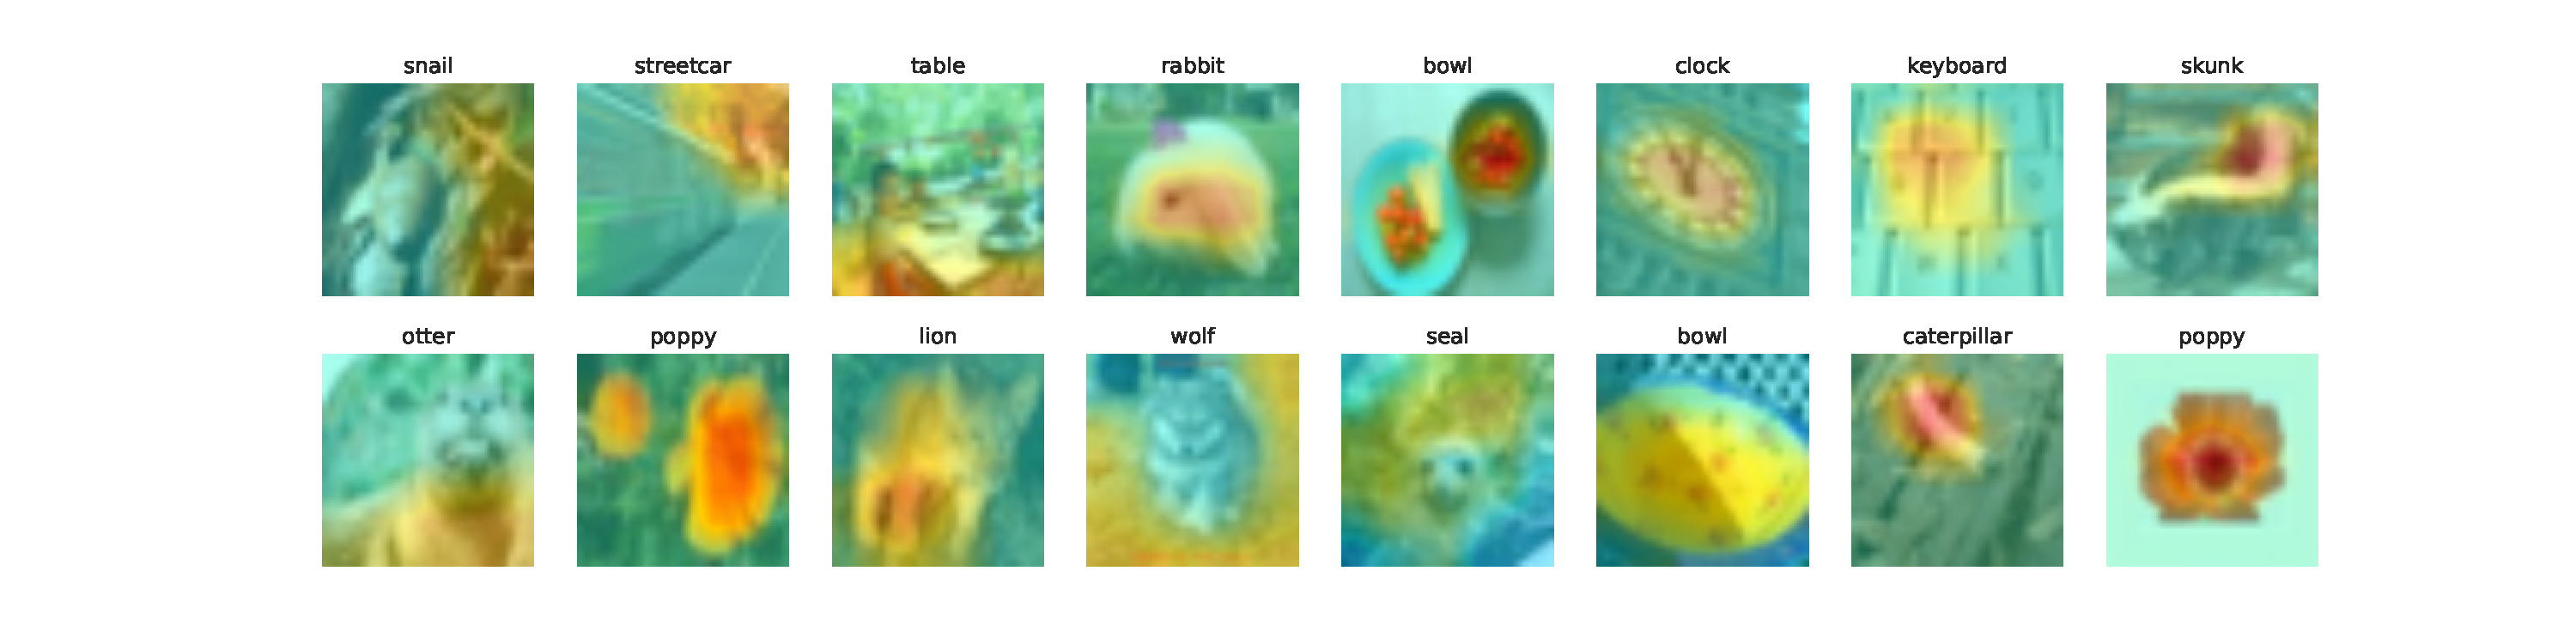
\includegraphics[width=\textwidth]{images/cifar100_efficientnet_b0_noproxy_0.pdf}
            \caption{Without Proxy Attention}
        \end{subfigure}
        \hfill
        \begin{subfigure}[b]{1\textwidth}
            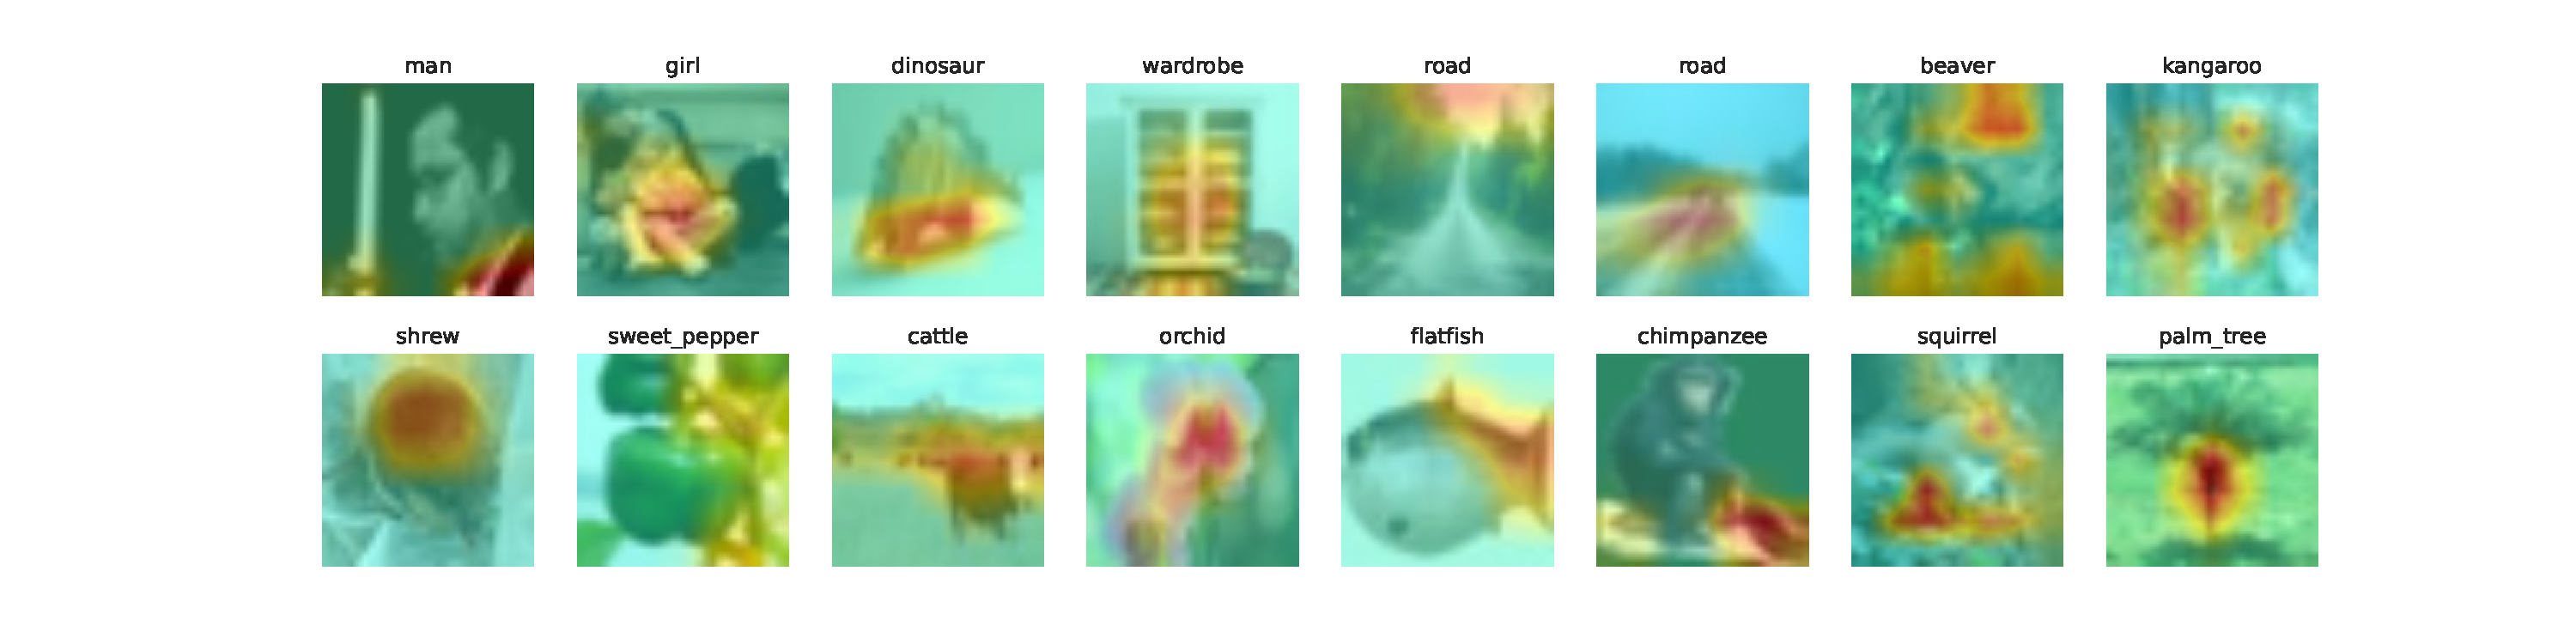
\includegraphics[width=\textwidth]{images/cifar100_efficientnet_b0_proxy_0.pdf}
            \caption{With Proxy Attention}
        \end{subfigure}
        \caption{Comparison of attention maps generated by efficientnet\_b0 trained with and without Proxy Attention on the cifar100 dataset}
    \end{figure}
    


\subsection{Tsinghua Dogs, ResNet18, EigenGradCAM}


%\chapter{Discussion} \label{ch:discussion}
\section{Research Questions}
\begin{enumerate}
    \item Is it possible to create an augmentation technique that uses Attention maps?
    \item Is it possible to approximate the effects of Attention from ViTs in a CNN without changing the architecture?
    \item Is it possible to make a network converge faster and consequently require less data using the outputs from XAI techniques?
    \item Does using Proxy Attention impact the explainability positively?
\end{enumerate}

\section{General Discussion}
- optimizations , memory leaks
- managing computational resources and multiple experiments
- Improvements with better XAI techniques, better CNNs
%\chapter{Conclusion} \label{ch:conclusion}

\section{Lessons Learned}
The lessons learned from this thesis are as follows:
\begin{itemize}
    \item \textbf{Combining research from different domains to create a novel method: } This thesis taught me how to combine research from different domains to create a novel method. In this case, we combined research from the domains of XAI and Augmentation to create a novel augmentation technique.
    \item \textbf{Hyperparameter Tuning: } We performed a large number of experiments with different hyperparameters and models to test the robustness of the method and find the best configuration. Doing so taught me the importance of hyperparameter tuning.
    \item \textbf{Memory Leaks: }We encountered a lot of memory leaks while working on the code for this thesis, and in the process learned how to debug and fix them. 
    \item \textbf{Function based code: }We wrote the code for this thesis in a functional style instead of an object oriented style as a personal experiment (inspired by the success of the Julia programming language). This made it easy to reuse certain parts of the code and modify others. Doing so taught me the importance of writing functional code.
    \item \textbf{Augmentation: }We learned a lot about augmentation while working on this thesis. We learned about the different types of augmentations, how to implement them, and how to use them to improve the performance of CNNs.
    \item \textbf{XAI: }We also learned a lot about XAI while working on this thesis. 
    \item \textbf{Training Loop: } Previous to this thesis, the author had only used the training loop provided by higher level libraries. However, for this thesis, we had to implement the training loop from scratch. Doing so taught the author a lot about the different components of the training loop and how to configure them for optimal performance and modify them to suit the needs of the project.
\end{itemize}

\section{Future Work}
While the results of this thesis are promising, there is still a lot of room for improvement. The following are some of the possible future directions for this work:
\begin{itemize}
    \item \textbf{Schedules:} Currently, the number of Proxy Steps and the number of images used for the Proxy Step are fixed. It would be interesting to schedule both of these based on the validation performance. For example, if the validation performance is not improving, we can increase the number of Proxy Steps and the number of images used for the Proxy Step.
    \item \textbf{More XAI methods:} We have only used a tiny subset of XAI methods for this thesis. It would be interesting to experiment with more XAI methods (eg: other methods from the literature survey) and see if they can be used to improve the performance of Proxy Attention.
    \item \textbf{Smoothing Attention Maps:} The attention maps generated by the XAI methods are noisy. While no extra smoothing was used in this thesis, it would be useful to experiment with smoothing the attention maps before using them for the Proxy step. An example of a potentially suitable smoothing method is Eigen Smoothing \cite{jacobPyTorchLibraryCAM2021}.
    \item \textbf{Better Attention Maps for ViT:} This research used the base vision transformer model but Abnar et al. \cite{abnarQuantifyingAttentionFlow2020} in their paper, find that the attention maps generated by a vision transformer are pretty unreliable due to self attention, combining different representations across layers of the transformer. While using self attention does lead to massive improvements and performance for Transformers, using these attention weights is an unreliable method of generating proper explanations. Thus future work could take their work into account to have a better comparison between CNNs and Transformers.
\end{itemize}

%\chapter{Appendix}
\subsection{Summary of Results Per Dataset}
This section shows the accuracies per model for each dataset. The results are shown in Table ~\ref{tab:summary_ds}.
\begin{table}[H]
\centering
\resizebox{0.8\columnwidth}{!}{%
\begin{tabular}{lllr}
\toprule
         &                      &          &   accuracy \\
ds\_name & model & step\_schedule &            \\
\midrule
dogs & efficientnet\_b0 & Proxy &  94.630158 \\
         &                      & No Proxy &  85.605498 \\
cifar100 & vit\_base\_patch16\_224 & Proxy &  75.651538 \\
         &                      & No Proxy &  54.910000 \\
\bottomrule
\end{tabular}
}
\caption{Summary of results on different datasets}
\label{tab:summary_ds}
\end{table}


\chapter*{Key}

\begin{enumerate}
    \item $\odot$ denotes element-wise multiplication
    \item CNN denotes Convolutional Neural Network
    \item NLP denotes Natural Language Processing
    \item NN denotes Neural Network
    \item SOTA denotes State of the Art
    \item ViT denotes Vision Transformer
    \item XAI denotes Explainable Artificial Intelligence
    \item LR denotes Learning Rate
    \item LM denotes Language Modeling
    \item CV denotes Computer Vision
\end{enumerate}

\chapter{Introduction}

\section{Problem Statement}
The problem statement of this study is creating a novel augmentation technique \textbf{Proxy Attention}, that uses attention maps to improve the performance of any model by guiding its attention away from the regions that are not important for the classification task.
In turn, this method should also improve the explainability of the model while maintaining the same architecture and hyperparameters.

\section{Motivation}
Over the past few years, Transformers have slowly become the SOTA in a majority of NLP tasks. Recently, they have also started taking over the CV world. Dosovitskiy et al. \cite{dosovitskiyImageWorth16x162021}  modified the image pipeline to generate patches of images, hence mimicking the NLP pipeline required by the Transformer. Doing so led to the creation of Vision Transfer (ViT), variants of which have also been used to achieve SOTA results in image classification. However, ViTs are computationally expensive, harder to train, and require more data. While transfer learning can be used to mitigate the data requirement, CNNs are still extremely useful and are the go-to choice for many computer vision tasks.\\
One of the biggest advantages of Transformers is Attention, which helps it learn where to look in an image/text \cite{vaswaniAttentionAllYou2017}. The caveat of the boost in performance that attention brings, is offset by its computational cost. As Poli et al. \cite{poliHyenaHierarchyLarger2023} in their research on larger language models find, using attention is not always worth it. Bastings et al. \cite{bastingsElephantInterpretabilityRoom2020} compare the concepts of Attention maps from Transformers and Saliency maps from CNNs and find that Transformers do not always have much of an advantage in explainability. CNNs are still extremely useful, but they lack the inbuilt explainability of Transformers. A vast majority of CNNs that we use today rely on older concepts, and upgrading the principles behind them to fit more modern standards is not easy. An initial idea for this study was inspired by the work of Liu et al. \cite{liuConvNet2020s2022}, where the authors proposed a new architecture that uses many concepts from Transformers to improve the performance of CNNs. While this approach is promising, it requires a lot of changes to the architecture and hyperparameters and does not generalize well to other models. \\\\
The motivation behind Proxy Attention was to combine the best of both worlds. Since it is not directly possible without specialized architectures, we use XAI techniques to approximate the effects of attention and use it as a \textit{Proxy}. The idea behind Proxy Attention stems from the following intuition: the mistakes made by CNNs are often due to the model focusing on the wrong regions of the image. While CNNs eventually learn to understand the images better and choose the right regions, this requires quite some training time. Proxy Attention aims to slightly speed up this process, and eventually make the model converge faster by gently guiding its attention away from the regions that are not important for the classification task.\\
Proxy Attention uses what the model already knows to help guide it by helping it better understand its mistakes. Using XAI techniques, the regions that the model used to make its prediction can be identified. If the image was misclassified, we can say that the model probably focused on the wrong regions. Using this information, we can re-weight the image to minimize the effect of the regions that most strongly influenced the prediction. Since the model is already familiar with the image, showing it a modified version of the image should potentially help it generalize better.\\
This research further explores the idea of Proxy Attention and tests its effect on the performance and explainability of standard models for classification tasks. No method is perfect, and Proxy Attention is no exception. That being the case, we also explore some of the limitations of Proxy Attention and discuss possible solutions to mitigate them.

\section{Context and Novelty}
The concept of Proxy Attention is relevant to any computer vision task, but we focus on image classification in this study. Using Proxy Attention, significant improvements in performance and explainability can be achieved without changing the architecture and with minimal changes to an existing code base.\\
The novelty of this study is the use of XAI techniques as an augmentation technique to approximate the effects of Attention in a CNN and guide the model's focus away from the regions that are preventing it from making the correct prediction. Proxy Attention was created in the hopes of showing that the explainability of CNNs can be improved by using the outputs from XAI techniques.\\
Combining these two concepts is a novel approach, and the author hopes that this study will inspire further research in this direction and motivate researchers to explore the possibilities of combining seemingly unrelated concepts to create novel solutions.

\section{Contributions}
The contributions of this thesis are as follows:
\begin{itemize}
    \item \textbf{Novel augmentation technique that uses attention maps: } We proposed a novel, easy to implement augmentation technique - \textit{Proxy Attention} that uses attention maps generated by XAI methods to emulate Attention in CNNs. We showed that this technique can be used to improve the performance of CNNs without any change in the architecture. We also showed that Proxy Attention improves the explainability of the model with minimal computational overhead.
    \item \textbf{Robustness: } We performed a large number of experiments with different hyperparameters and models to test the robustness of the method and find the best configuration. 
    \item \textbf{Open source callback code: } We have open sourced the callback code that can be used to easily add Proxy Attention to any existing code base.
    \item \textbf{Tensorboard Log Parser: } We have also open sourced a script to easily parse tensorboard logs to a unified DataFrame for easy analysis. This script was used to generate the plots and tables in this thesis.
    \item \textbf{Reproducibility: } All the scripts used for this thesis along with the training logs are available for open source. This makes it easy to reproduce all the results in this thesis.
\end{itemize}


\section{Challenges}
The major challenges of this study were as follows:
\begin{enumerate}
    \item Creating a novel augmentation technique that uses attention maps to improve the model's performance.
    \item Testing the effect of Proxy attention on the explainability of the model.
    \item Comparing many hyperparameters and models with limited computational resources.
    \item Optimizing the usage of XAI techniques to improve the computational efficiency of Proxy Attention.
\end{enumerate}

\section{Research Questions} \label{section:researchq}
The main research questions that summarize the aims of this study are as follows.
\begin{enumerate}
    \item Is it possible to create an augmentation technique that uses Attention maps?
    \item Is it possible to approximate the effects of Attention from ViTs in a CNN without changing the architecture?
    \item Is it possible to make a network converge faster and consequently require fewer data using the outputs from XAI techniques?
    \item Does using Proxy Attention impact the explainability positively?
\end{enumerate}
\section{Thesis Outline}
This thesis follows the following structure:
\begin{itemize}
    \item \textbf{Chapter ~\ref{ch:sota}} provides the necessary background information and literature review of the relevant topics.
    \item \textbf{Chapter ~\ref{ch:implementation}} describes the methodology used in this study and the implementation details.
    \item \textbf{Chapter ~\ref{ch:results}} presents the results and answers the research questions.
    \item \textbf{Chapter ~\ref{ch:discussion}} discusses the results in the context of the research questions and provides recommendations for future work.
    \item \textbf{Chapter ~\ref{ch:conclusion}} concludes the thesis and talks about personal learnings.
    \item \textbf{Chapter ~\ref{ch:appendix}} provides additional details and results.
\end{itemize}

\chapter{State of the Art} \label{ch:sota}
This chapter discusses the current state of the art in the fields of Gradient-Based Explanations and Augmentations for CNNs. The chapter is divided into two sections, one for each of the fields. The first section discusses the various methods used to explain the predictions of CNNs. The second section discusses the various methods used to augment the training data for CNNs. This chapter also discusses the limitations of the current methods and the motivation behind Proxy Attention.

\section{Gradient Based Explanations} \label{sec:gradient_based_explanations}
\subsection{Need For Explainability}
With the massive influx of new AI technologies and public use of these advanced technologies, being able to have some way to determine how well the systems perform outside the standard metrics is very important. The field of XAI aims to provide these explanations and in the process, enable stakeholders to have a higher trust in the AI models given to them. The following subsection lists some of the major reasons for using XAI techniques for any AI research project.
\begin{itemize}
    \item \textbf{Fairness: } What a model learns depends to a large degree on the dataset that it was trained on. That being the case, if the dataset is biased towards a certain class, the model might learn that bias during training. Examples include - Not having people of color in a face recognition dataset, having gendered examples in a formal clothing dataset, etc. XAI can help find these biases before a model is shipped to production.
    \item \textbf{Safety: } In safety-critical systems such as self-driving cars or medical diagnosis, knowing what factors led a model to provide a certain output is extremely important. Even if the system is partially operated by a human expert, having incorrect predictions could potentially lead to fatal decisions. XAI can be used to provide the required insights and prevent potentially harmful outcomes.
    \item \textbf{User Experience: } Since most real-world models are used in collaboration with human experts, having explanations makes the job of the human much easier and increases trust in the decisions provided by the model.
    \item \textbf{Better Model Performance: } Once we understand why a model is making certain mistakes, we can try to adjust the model or the data it is trained on to correct these issues. Using XAI techniques, it is possible to identify issues with the data or the models in question and potentially improve performance. (A good case in point is the research done for this paper - Proxy Attention.)
    \item \textbf{Regulatory Compliance: } Some regulations require decisions made by AI systems to be explainable. GDPR, for instance, includes a "right to explanation" of automated decisions. Since these policies are important in a societal setting, having these explanations as part of any model might help prevent legal issues. Note that GDPR and other similar rules require explainability to prevent companies from releasing models without appropriate testing.
    \end{itemize}

\subsection{Literature}
\textbf{Saliency Map: } The earliest mention of Saliency Maps was made in a book by Koch et al. \cite{ullman1988attention}. They proposed a means of measuring attentional control in organisms based on a combination of visual features. The Saliency Map in this case refers to a topographically oriented map of these combined features that can be used to determine how different a specific location would be from its surroundings based on the visual features. Koch et al. did not perform any practical research and were unrelated to the field of deep learning. Although the name Saliency map was proposed by them, the term is used interchangeably with that of the Saliency map proposed by Simonyan et al. \cite{simonyanDeepConvolutionalNetworks2014}.

\textbf{CAM: } Another one of the most popular gradient-based XAI methods, Class Activation Mapping (aka CAM) was proposed by Zhou et al. \cite{zhouLearningDeepFeatures2016}. CAM relies on modifying the architecture of the classification network by adding a Global Average Pooling layer and a linearly combined version of the class weights and the feature map to produce a class activation map. Compared to previous approaches, Zhou et al. focused on the visuals produced for an explanation and also mentioned that zeroing out the negative gradients for the backward step produces more appealing results.

\textbf{GradCAM: } The last conv layer before the final dense layer can be thought to have been learned from the combined knowledge of the entire network and can thus be used to produce a course saliency map. Thus in GradCAM \cite{selvarajuGradCAMVisualExplanations} the gradient is only back-propagated till the last conv layer. Another advantage of GradCAM is that it provides class-wise activation maps for a chosen class $c$. To do so, only the class activations for $c$ are used for backpropagation. A global average pooling is also used, weighted by the gradient. A class-specific heat map can then be generated from this information by passing the weights through a ReLU function. It is to be noted that the generated heat map is not the same size as the image but is smaller, and has to be mapped back to the dimensions of the original input.

\textbf{DeconvNet: }
One of the earlier approaches to Saliency maps for CNNs was proposed by Zeiler et al. \cite{zeilerVisualizingUnderstandingConvolutional2013} termed DeconvNet. DeconvNet works by inverting the network's operations in the forward pass. After attaching the DeconvNet layers to the network, propagating through these layers represents features that the original CNN possessed. The relevant reconstruction can be obtained for a single class by setting all the activations other than the one corresponding to the class to zero. The resulting image is then used to generate the saliency map. A Deconv layer replaces the Conv layer, and the ReLU operation has negative values clamped. While the pooling operation is not strictly invertible, the authors use switch variables that store the maximum value position for each pooling operation. While the DeconvNet works to a certain extent, the results are less accurate than the ones obtained by other methods and are also biased towards the representations of the first layer.

\textbf{Vanilla Gradient: }
Building on the DeconvNet, Simonyan et al. \cite{simonyanDeepConvolutionalNetworks2014} extrapolate the idea of class visualization to create one of the first approaches to Saliency maps. Their approach, also called Vanilla Gradient, ranks the pixels of an image $I_{0}$ by how important they are in the prediction of the Saliency score $$S_{c}(I) \approx w^{T}I + b$$. In this equation, $w$ and $b$ are the network weights and biases obtained by back-propagating wrt the image itself. The objective to be minimized thus is $$arg \underset{I}max S_{c}(I) - \lambda||I||^{2}_{2}$$ where $\lambda$ is used as a regularization parameter. Using these equations, a saliency map $A \in \mathbb{R}^{m \times n}$ ($m \times n$ stands for $height \times width$) can be computed. To find the map, we find the derivative of $w$, rearrange the elements, and then process them according to the number of input channels. If the number of channels is greater than one, the maximum value over the channel is considered $$A_{i,j}= \underset{ch}max |w_{h_{(i,j, ch)}}|$$. Where $ch$ is the color channel of the pixel $(i,j)$, $h(i,j, ch)$ is the index of the $w$ corresponding to that pixel. The Vanilla Gradient method produces an approximate saliency map but has much noise. This leads to issues for more complex images. The methods proposed in the following papers have addressed many of the issues with Vanilla Gradients and DeconvNets \cite{zeilerVisualizingUnderstandingConvolutional2013}.

\textbf{ScoreCAM: }
In another paper, the authors propose a score-weighted approach - ScoreCAM to create saliency maps \cite{wangScoreCAMScoreWeightedVisual2020}. Like many other methods, the images are first passed through the network, and the corresponding activations are obtained from the final convolutional layer. These activation maps are upsampled and normalized to $[0,1]$. The highlighted activation map portions are then passed through a CNN with a softmax layer to obtain the score for each of the current classes. These scores are used to find the activation maps' relative importance. Finally, the sum of all these maps is computed using a linear combination with the corresponding target score and then passed through a ReLU operation. These operations can be mathematically represented as $$L^{c}_{ScoreCAM} = ReLU(\underset{k}\Sigma w_{k}^{c}A^{k})$$, where $k$ represents the index considered, $c$ represents the current class and $S_k$ represents the outputs of the SoftMax as mentioned earlier layer. The authors find that the maps obtained using ScoreCAM are less noisy, and this method removes the dependency on unstable gradients compared to other methods.

\textbf{Guided Gradcam: }
A variant of GradCAM \cite{selvarajuGradCAMVisualExplanations} was proposed by Selvaraju et al. \cite{selvarajuGradCAMWhyDid2017} where, unlike GradCAM that finds the parts of the image that influence the model's decision, Guided GradCAM takes the positive gradients into account. These gradients are used to obtain an even more fine-grained representation of the outputs of the saliency map. While GradCAM backpropagates both positive and negative gradients, Guided Backprop only propagates the positive gradients and is defined as a pointwise multiplication of the results of GradCAM and Guided Backpropagation \cite{springenbergStrivingSimplicityAll2015}.

\textbf{Guided Backprop: } Guided Backprop (GBP) \cite{springenbergStrivingSimplicityAll2015} can be thought of as a combination of the ideas of DeconvNets \cite{zeilerVisualizingUnderstandingConvolutional2013} and Vanilla Gradients \cite{simonyanDeepConvolutionalNetworks2014}. Since the DeconvNet does not take negative gradients into account, it suffers from a loss in performance for the higher layers in the network. Springenberg et al. propose masking all the negative values in the ReLU function applied by DeconvNet. They use the DeconvNet mask and apply it to the output of the Vanilla Gradient method to remove the noise that the latter creates. Doing so enables GBP to generate clearer images than the other two methods. Note that GBP is applied across the entire network and not only the first layer.

\textbf{GradCAM++: } GradCAM++ \cite{chattopadhayGradCAMGeneralizedGradientBased2018} improves upon the original GradCAM method by considering both first-order and second-order gradients. Considering both allows GradCAM++ to gather more detailed information about the significance of each pixel in an input image. The second-order gradients of the target class are computed in relation to the final convolutional feature maps. These gradients are then multiplied with each other, and are used as importance scores. GradCAM++ uses these scores to generate a more accurate heatmap, highlighting the most distinguishing areas in the image. GradCAM++ also introduces a self-correcting mechanism that uses positive gradient information obtained from the other classes to enhance localization precision which in turn rectifies any potential localization errors.

\textbf{Noise Tunnel: }
In combination with attribution methods, Noise Tunnel \cite{kokhlikyanCaptumUnifiedGeneric2020} is an algorithm that improves the accuracy of the masks obtained by these methods. Noise Tunnel was proposed to counter noisy and irrelevant attributions obtained by some gradient-based methods by adding a Gaussian Noise and then averaging the predictions over sampled attributions. Since all the samples are considered, this method has a significant computational overhead. For Smooth Grad \cite{smilkovSmoothGradRemovingNoise2017}, the new attribution is defined as $$\hat M_{c}(x) = \frac{1}{n}\Sigma_{1}^{n}M_{c}(x + \mathcal{N}(0, \sigma^{2}))$$. Where $M_{c}$ is the attribution calculated by SmoothGrad, $\mathcal {N}(0, 0.01^2)$ is the Gaussian Noise with $\sigma = 0.01$ and $n$ is the number of samples. Similarly for Smooth Grad Square, $$\hat M_{c}(x) = \frac{1}{n}\Sigma_{1}^{n}\sqrt{M_{c}(x + \mathcal{N}(0, \sigma^{2}))}$$. Noise Tunnel can also be used on Var Grad \cite{richterVarGradLowVarianceGradient2020} with the equation $$\hat M_{c}(x) = \frac{1}{n}\Sigma_{k=1}^{n}\{M_{c}(x + \mathcal{N}(0, \sigma^{2}))\}^{2}- \{\hat M_{c}(x)\}^{2}$$

\textbf{Integrated Gradients: }
For a model $F$, the attribution method Integrated Gradients \cite{sundararajanAxiomaticAttributionDeep2017} computes the contribution of each pixel in the image towards the final prediction. The model's output is used to calculate a pixel-wise partial derivative that is then integrated along a path starting from the baseline and ending at the input. Each step is scaled according to the partial derivative obtained in the previous step. For every step k with m total steps over the path, the IG equation is defined as $$IntegratedGrads_i^{approx}(x) =(x_{i}-x_i')\times \Sigma_{k=1}^{m}\frac{\partial F(x' + \frac{k}{m} \times (x-x'))}{\partial x_{i}} \times \frac{1}{m}$$. Where $(x_{i} - x_{i}')$ is the pixel-wise difference between the two images, $$\frac{\partial F(x' + \frac{k}{m} \times (x-x'))}{\partial x_i}$$ is the partial derivative of the model output $F$ for pixel $i$ at the $k$-th step of the path, and $\frac{1}{m}$ is the scaling factor that ensures that each of the steps taken contributes equally to the final result.

\textbf{Conductance: }
Building upon Integrated Gradients, Dhamdhere et al. propose \cite{dhamdhereHowImportantNeuron2018} Conductance, a means to boost the attributions provided by IG to specific neurons in the hidden layer. This is done by decomposing the computation that IG performs. The authors apply this method to the Inception network \cite{szegedyGoingDeeperConvolutions2014} and can find the filters that influence the final predictions the most. 
For a neuron $y$, the network can be represented as a function $F: R^{n} \rightarrow [0,1]$. Given an input $x \in R^{n}$ and a baseline input $x' \in R^{n}$, the IG for the $i^{th}$ dimension at $x$ is given by $$IG_{i}(x) = (x_{i}- x_{i}') \int_{\alpha=0}^{1} \frac{\partial F(x' + \alpha(x-x'))}{\partial x_{i}}d \alpha$$ . Considering $\frac{\partial F(x)}{\partial x_{i}}$ to be the gradient of $F$ along $i^{th}$ dimension at x, the Conductance for $y$ can be defined as $$
Cond_{i}^{y}(x) ::== (x_{i}- x_{i}') \int_{\alpha=0}^{1} \frac{\partial F(x' + \alpha(x-x'))}{\partial y} \cdot \frac{\partial y}{\partial x_{i}} d \alpha$$. The authors also propose methods of evaluating Conductance by the assumption that an influential hidden network should be good at predicting the given input class. This assumption can be validated by two metrics: the $$Gradient\times Activation = 
y \times \frac{\partial F(x' + \alpha \times (x-x'))}{\partial y} d \alpha$$ and the Internal Influence : $$
IntInf ^{y}(x) = \int^{1}_{\alpha=0} \frac{\partial F(x' + \alpha(x-x'))}{\partial y} d \alpha$$.\\
\textbf{RISE: }
Petsiuk et al. propose RISE \cite{petsiukRISERandomizedInput2018}, a saliency method that randomly alters the input images by applying random noise to each. After model predictions are obtained, the saliency map is generated by combining the partial maps over each modified image. RISE improves accuracy but needs a lot of computation time, considering that multiple models must be trained for each random noise sample.

\textbf{Influence Of Image Classifican Accuracy On Saliency Map Estimation: }
Oyama et al. \cite{oyamaInfluenceImageClassification2018} found a strong correlation concerning the relationship between saliency maps and image classification accuracy. The authors found that the architecture and the initialization strategy influence the final saliency map. By analyzing the generated saliency maps, they find that if the model is randomly initialized and trained for image classification, having limited categories in the original dataset leads to overfitting. On the other hand, having many categories suppresses the overfitting of the objects present in the training dataset. On training their proposed network ReadoutNet on a fixation task (which requires the network to learn where to focus), they found that the accuracy of estimating the saliency map was linked to the image classification accuracy.

\textbf{Summit: }
While a large amount of research focuses on interpreting the influence of a single image or neuron, Hohman et al. propose Summit, \cite{hohmanSummitScalingDeep2019} a novel scalable summarization algorithm. Summit creates an attribution graph that distills the influence of neurons and substructures throughout the network used to make the final prediction. The attribution graph is created due to combining activation aggregation, a technique to find important neurons, and neuron-influence aggregation, a technique to find relationships among the neurons identified in the previous step. After a forward pass through the network, the activation channels maximums are obtained to aggregate the activations. These are then filtered by class and aggregated by taking the top $k$ channels or the top $k$ channels by weight. To quantify how much a layer influences the next, the authors aggregate the influences by creating a tensor $I^{l}$ for all the network layers ($l$). How important channel $i$ of the layer $l-1$ is determined by the aggregate tensor $I^{l}_{cij}$ where $j$ represents the output channel and $c$ is the class of the image. Considering the $j^{th}$ kernel of the layer $K^{(j)} \in \mathbb{R}^{H \times W \times C_{l-1}}$, a single channel $Y$ can be represented using the 3D convolution operation by $Y_{:,:,j}= X \ast K^{(j)}$. This is equivalent to it's representation by the 2D convolution $$Y_{:,:,j}= \Sigma_{i=1}^{C_{l-1}} X_{:,:,i} \ast K^{(j)}_{:,:,i}$$. The value $X_{:,:, i} \ast K^{(j)}_{:,:, i}$ is the contribution of the current channel from the previous layer and the maximum of this value is used to generate the influence map.

\textbf{Smooth Grad: }
Consider an image classification task where an input image $x$ is classified as a single class from a set $C$. For every class $c \in C$, the output class is represented as $class(x) = argmax_{c \in C}S_{c}(x)$. Using this $class$, a sensitivity map $M_{c}(x)$ can be generated by differentiating with respect to $x$, $$M_{c}(x) = \frac{\partial S_{c}}{\partial x}$$ . $M_{c}$, being a sensitivity map \cite{simonyanDeepConvolutionalNetworks2014}, thus representing the influential regions of the image used to make the prediction. Since these maps are noisy, Smilkov et al. propose SmoothGrad \cite{smilkovSmoothGradRemovingNoise2017}, a modification of the previous method where instead of using $\partial S_{c}$, a smoothing is applied using a Gaussian kernel to $\partial S_{c}$. The authors also find that it is impossible to directly compute the smoothing due to high dimensionality and thus approximate the calculation by averaging multiple maps computed in the neighborhood of $x$ using random sampling. The final SmoothGrad equation then becomes $$\hat M_{c}(x) = \frac{1}{n}\Sigma_{1}^{n}M_{c}(x + \mathcal{N}(0, \sigma^{2}))$$, where $\mathcal{N}(0, \sigma^{2})$ is the Gaussian noise and $\sigma$ is the standard deviation.

\textbf{Deep Visual Explanations: }
The ability of a model to explain the reason for its predictions in the context of an image classification task is known as Deep Visual Explanation (DVE). Babiker et al. \cite{babikerIntroductionDeepVisual2018} propose a method to generate DVEs by using the activation of different spatial scales in the Fourier space. Since CNNs generate spatial information at different layers, the authors use this information in the form of feature maps to generate explanations. The activations that do not contribute to the final prediction are penalized and the final explanation is generated by combining the activations of the high and low spatial scales in the aforementioned Fourier space. Combining the explanations provided by these two scales allows the authors to generate a more targeted explanation.

\textbf{Embedding Knowledge Into Deep Attention Map: }
Mitsuhara et al. \cite{mitsuharaEmbeddingHumanKnowledge2019} propose an approach that involves manually editing the attention maps generated by the network to provide the model with expert human input. They use an Attention Branch Network (ABN), fine-tune it using the manually edited attention maps, and then use the fine-tuned model to generate the final attention map. The authors also demonstrate a tool that can be used to interactively modify the attention maps using a mouse. This tool takes misclassified images as input and allows the user to add or remove attention regions before passing the edited attention map to the network. The authors also demonstrate that the fine-tuned model performs better than the original model due to the additional expert input.

\textbf{Sam ResNet: }
Another approach to creating attention maps involves using an LSTM as part of a method called SAM \cite{corniaPredictingHumanEye2018} . The authors use a ResNet to extract feature maps from the input image, which are then passed to an Attentive Convolutional LSTM for refinement. A separate module is used to add priors to the attention map to account for the center bias present in human eye fixations. Many advantages that LSTMs provide are used in the research, such as the ability to process features iteratively. The attention map is generated with a convolution of the previous hidden state and the input, which is then normalized using the softmax operator. The authors find that the attention maps generated by SAM are quite accurate and using a modified version of the ResNet, they can generate attention maps that are of higher resolution.

\textbf{Eigen CAM: } Another method for computing Saliency Maps without modifying the architecture of the network, EigenCAM was proposed by Bany et al. \cite{banymuhammadEigenCAMVisualExplanations2021}. EigenCAM uses a combination of an Eigen decomposition of the class-activated output by projecting it on the input, and a PCA of it to remove unnecessary features from the maps. The Eigen-Saliency map is computed across the network and produces sharper outputs based on the distance (using PCA) from the input image. EigenCAM and Eigen Saliency maps were fused by a point-wise multiplication operation.

\section{Augmentation} \label{sec:augmentation}
\subsection{Need for Augmentation}

A good dataset is the bread and butter of a high-performing deep learning model. That being the case, it is not always possible to have a large data set, especially for niche tasks. This is where augmentation comes into play. The major idea behind augmentation is to generate more images given an existing dataset where the newly generated images belong to the same distribution as the other images in the dataset. Using augmentation techniques, it is possible to increase the size of datasets where there are few annotated samples present. It is also to be noted that these augmentation techniques are independent of the task at hand, except for cases where the operations do not translate well over to a different task. For instance, cropping, an image would make sense in an image classification task, but in the case of a semantic segmentation task, performing a naive crop without any other metrics might lead to negative performance. Yang et al. \cite{yangImageDataAugmentation2022} proposed a hierarchy of data augmentation techniques in their paper, which is referred to for the below classification. (Also refer to Figure ~\ref{fig:categorization_augmentation} for more information.)

\textbf{Classification of Augmentation techniques}:
\begin{itemize}
\item \textbf{Image Erasing :} This operation refers to deleting subregions of the images to generate newer images. The deleted regions can be replaced with values ranging from complete zeros, random numbers, or any other parameter. Examples include : \cite{zhongRandomErasingData2020,chenGridMaskDataAugmentation2020,singhHideandSeekDataAugmentation2018} etc.
\item \textbf{Image Mix :} Image mixing refers to the operation where multiple images have their subregions merged. The amount of mixing and the method of mixing these images are different for every method. An example of such an image of mixing augmentation technique is MixUp \cite{zhangMixupEmpiricalRisk2018}.
\item \textbf{Image Manipulation :} Image manipulation refers to any operation that modifies the image geometrically, such as rotating or flipping the image, cropping, etc. An example of Image Mixing is CutMix \cite{yunCutMixRegularizationStrategy2019a}.
\item \textbf{Auto Augment :} Auto Augmentation refers to methods that instead of taking a fixed parameter or augmentation technique, perform a grid search over a set of parameters and techniques to find one that performs the best. Since the search space is potentially extremely large, these methods attempt to manipulate the order of searches or attempt to narrow down the search space to be able to find the best method. One of the most popular auto augmentation techniques is RandAugment \cite{cubukRandaugmentPracticalAutomated2020}.
\item \textbf{Feature Augmentation :} Another method of augmentation involves manipulating transformations in the feature space instead of the input space like the other methods. These methods work on the following principle - since the images come from the same dataset, they are expected to be from the same distribution. (This distribution can be thought of as a data manifold.) While traversing this data manifold, it is possible to find other similar examples that could also potentially belong to the same data distribution, thereby generating new samples that also fall in the same distribution as the original dataset. An example would be \cite{devriesImprovedRegularizationConvolutional2017}.
\item \textbf{Deep Generative Models :} GANs are a family of models that essentially perform the same task as feature augmentation, whereby they attempt to generate images that belong to the same distribution as the input data set. Since the generated images are similar to the images that were given to the network to learn in the first place, but not the same, it is possible to use these outputs as images for data augmentation. It is to be noted that using these images directly might not always be a good idea because GANs sometimes produce noisy outputs that might lead to network learning features that are not relevant. Some examples of GANs that can be used for Data Augmentation are \cite{choiStarGANV2Diverse2020,isolaImagetoImageTranslationConditional2018}.
\end{itemize}

\begin{figure}[!htb]
    \centering
    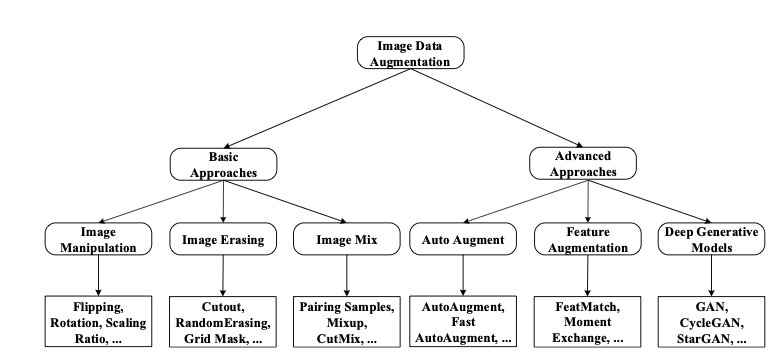
\includegraphics[width=.9\textwidth]{images/data_aug_categories.png}
    \caption{Taxonomy of Data Augmentation (sourced from \cite{yangImageDataAugmentation2022})}
    \label{fig:categorization_augmentation}
\end{figure}

\subsection{Literature}
\textbf{AugMix: }
Another augmentation strategy proposed by \cite{hendrycksAugMixSimpleData2020} first applies multiple transformations randomly and in parallel chains to each image. These transformations can include combinations of Translation, Rotation, Shearing, and others. The outputs of these combinations are then mixed to form a new image, which is further mixed with the original image to form the new image. This combination improves performance in cases where data shifts are encountered in production. Once the images are mixed, a skip connection is used to combine the results of the chains. AugMix also uses the Jensen-Shannon Divergence consistency loss \cite{linDivergenceMeasuresBased} to ensure the images are stable across various inputs. Considering $KL$ to be Kullback-Leibler Divergence, the Jensen-Shannon Divergence can be defined as $$
    JS(p_{orig}; p_{augmix1};p_{augmix2}) = \frac{1}{3}(KL[p_{orig}||M||]+KL[p_{augmix1}||M||]+KL[p_{augmix2}||M||])
$$, where $M$ is the mean of the three distributions $p_{orig}, p_{augmix1}, p_{augmix2}$.

\textbf{Cutout: }
Devries et al., in their paper \cite{devriesImprovedRegularizationConvolutional2017}, propose an augmentation method they call Cutout. This method removes random-sized square patches from the images by replacing the corresponding pixels with a constant value (usually 0). Selecting the region involves picking a random pixel value and creating a uniform-sized square around the chosen pixel. The authors also find that Cutout performs better with other methods than just being used by itself. Cutout can be expressed as an element-wise multiplication operation $$x_{cutout} = x \odot M$$,
$x$ is the original image, $M$ is a binary mask of the same size as $x$ with randomly chosen coordinates of a square patch of pixels to be cut out, and $\odot$ denotes element-wise multiplication.

\textbf{Cut and Mix: }
Unlike Cutout \cite{devriesImprovedRegularizationConvolutional2017}, where the chosen patch is replaced with zero pixels, in CutMix \cite{yunCutMixRegularizationStrategy2019}, the chosen patch is replaced with a randomly chosen patch from a different region of the same image. Yun et al. propose this approach as multiple class labels can be learned with a single image.
CutMix can be defined by the following operations $$\overset{\sim}x = M \odot x_{A} + (1-M) \odot x_{B}$$ ; $$\overset{\sim}y = \lambda y_{A}+ (1- \lambda)y_{B}$$. $x$ is an RGB image, $y$ is the respective label, $M$ is a binary mask of the image patch that will be dropped, and $\odot$ represents element-wise multiplication. The new training sample $\overset{\sim}x , \overset{\sim}y$ is created by combining two other training samples $x_{A}, y_{A}$ and $x_{B} , y_{B}$. To control the combination ratio $\lambda$, a sample from the $\beta(1,1)$ distribution is chosen. This combination is quite similar to \cite{zhangMixupEmpiricalRisk2018} but differs in the sense that CutMix focuses on generating locally natural images.

\textbf{Attentive Cutmix: }
Building upon \cite{yunCutMixRegularizationStrategy2019}, Walawalkar et al. propose an alternative method of replacing patches in an image they call Attentive CutMix \cite{walawalkarAttentiveCutMixEnhanced2020}. Instead of randomly pasting patches in the image, this method uses a pre-trained network to identify attentive regions from the image. Similar to the earlier approach, these patches are mapped back to the original image. Doing so allows the network to select important background regions for the task while also updating the label information.

\textbf{Cow Mask: }
Many of the algorithms use rectangular or square-shaped masks. While effective, French et al. propose Cow Mask \cite{frenchMilkingCowMaskSemiSupervised2020}, a new masking method that uses irregularly shaped masks with a Gaussian filter to reduce noise. The authors also propose two mixing methods, one that builds up on Random Erasing \cite{zhongRandomErasingData2020}, and another that uses Cut Mix \cite{yunCutMixRegularizationStrategy2019}. A pixel-wise mixing threshold is also chosen, and either mixing or erasing is applied to the image based on this threshold. This augmentation technique is shown to be effective in semi-supervised learning.

\textbf{Cut Paste Learn: }
Dwibedi et al. proposed another approach involving a cut-paste methodology \cite{dwibediCutPasteLearn2017}. In their paper, the authors propose a new method of augmentation that extracts instances of objects from the images. Instead of pasting them on other images, they are pasted on randomly chosen backgrounds. This method leads to pixel artifacts in the images, as selecting the objects is a noisy process. To overcome the drop in performance, the authors apply a Gaussian blur and Poisson blending to the boundaries of the pasted objects. Further augmentation is applied before pasting the objects by rotation, occlusion, and truncation. The authors also find that this approach makes the network more robust to image artifacts.

\textbf{Hide and Seek: }
In their paper, Singh et al. \cite{singhHideandSeekDataAugmentation2018} propose a data augmentation method that takes an image as an input and divides it into a grid. Each of the sub-grids is then turned off with a given probability. These sub-grids can be connected or independent of each other, and the turned-off grids are replaced by the average pixel value of all the images in the dataset.

\textbf{GridMask: }
One of the major drawbacks of algorithms that rely on modifying image patches (such as \cite{singhHideandSeekDataAugmentation2018,devriesImprovedRegularizationConvolutional2017,zhongRandomErasingData2020}) is that they sometimes delete parts of the image that might be useful to the network. To overcome this problem, Chen et al. propose a new method Grid Mask \cite{chenGridMaskDataAugmentation2020}, that uses evenly spaced grids to find a balance between the amount of information that is deleted and stored. Using the number of grids and their respective sizes as a hyperparameter, the authors find that Grid Mask effectively preserves important parts of the image.

\textbf{Intra-class Part Swapping: }
Zhang et al. propose a data augmentation method called Intra-class Part Swapping \cite{zhangIntraClassPartSwapping2021} that uses a CAM \cite{zhouLearningDeepFeatures2016} to identify the most important regions of an image. These parts are then thresholded, scaled, translated, and pasted onto the target image. A similar process is also applied to the target image, and the attentive parts of the original image are used to replace the corresponding attentive parts of the target image. Similar to previous methods, the labels are also updated to reflect the changes in the image.

\textbf{Random Erasing: }
While Cutout augmentation \cite{devriesImprovedRegularizationConvolutional2017} is applied to every image in the dataset, Zhong et al. propose a new method, Random Erasing, that takes a probability of being applied into account \cite{zhongRandomErasingData2020}. In Random Erasing, contiguous rectangular regions are selected and replaced randomly with random upper and lower limits chosen for both region area and aspect ratio. A region-aware detection algorithm is applied for object detection tasks to make the network more robust to occlusion. Note that Cutout removes square patches, while Random Erasing removes square or rectangular patches.

\textbf{ResizeMix: }
Many augmentation methods that rely on randomly choosing regions to cut and paste from sometimes fail to work well with regions that need more object information. ResizeMix \cite{qinResizeMixMixingData2020} tackles this problem by replacing the patch with a proportionally resized version of the selected image. This method is similar to CutMix \cite{yunCutMixRegularizationStrategy2019} but differs in the sense that ResizeMix uses a resized version of the entire image instead of a randomly chosen patch.

\textbf{RICAP: }
Another augmentation technique that applies random cropping and pasting is RICAP \cite{takahashiDataAugmentationUsing2020}. In this method, four regions are cropped from different images and pasted together to form a new image. The created image thus has multiple mixed labels. A uniform distribution is used to determine the area of each cropped region in the final image. The authors propose multiple variants of RICAP that use different points of origin for cropping. The method works best when the cropped regions use the corners as the origin, allowing the network to see more of the image.

\textbf{Sample Pairing: }
In their paper, Inoue et al. propose a method that merges images not by cut and paste but by averaging their pixel intensities. While algorithms like Mixup \cite{zhangMixupEmpiricalRisk2018} modify the image's labels proportional to the amount of mixing between the original and the target images, Sample Pairing \cite{inoueDataAugmentationPairing2018} maintains the same training labels. Sample Pairing follows an interval-based augmentation policy, where the network is trained for 100 epochs before being introduced to the mixed images. This process is also repeated cyclically with eight epochs of training with mixed images followed by 2 epochs of training with normal images.

\textbf{Smooth Mix: }
With the success of mask-based approaches for data augmentation, there have been many papers that attempt to fix the flaws of previous research. One such method is SmoothMix \cite{leeSmoothMixSimpleEffective2020}, which builds up on both CutMix \cite{yunCutMixRegularizationStrategy2019} and Cutout \cite{devriesImprovedRegularizationConvolutional2017} but modifies the mask to have softer edges. The intensity of the masked edges gradually decreases and depends on the strength of the mask. The updated pixel values are thus obtained by mixing the mask with the original image according to the formula $$\lambda= \frac{\Sigma_{i=1}^{W}\Sigma_{j=1}^{H}G_{ij}}{WH}$$. Where $G_{ij}$ is the pixel value of mask $G$ and $H, W$ are the height and width of the image, respectively. The new pixel values are then $$(x_{new} , y_{new}) = (G.xa + (1 - G).xb , \lambda.ya + (1 - \lambda).yb)$$

\textbf{SMOTE: }
One of the older data augmentation methods is SMOTE \cite{SMOTESyntheticMinority}. This algorithm is not domain specific, but in the context of computer vision, it can be used to balance datasets that suffer from imbalanced labels. SMOTE generates new samples by combining the K-nearest neighbors of the minority class images to form new instances. Although many of the other methods discussed in this paper are more effective, SMOTE is still useful.

\textbf{SnapMix: }
Huang et al. propose SnapMix \cite{huangSnapMixSemanticallyProportional2021}, where choosing the patch size to be cut is determined from the beta distributions of both the original and target images. The extracted patches are then merged with random image regions, each of which is different in size. Labels are also updated by taking the composition of the images into account.

\textbf{Remix: }
Cao et al. address the problem of class imbalance by performing data augmentation on images that are part of a minority class. From the labels of the images that were mixed, the final label is chosen as the label of the image with the least representation in the dataset. The authors call this method ReMix \cite{caoReMixImagetoImageTranslation2021}.

\textbf{Visual Context Augmentation: }
Dvornik et al. propose Visual Context Augmentation \cite{dvornikModelingVisualContext2018} that uses a NN to understand the context of objects in the image before pasting them in the target image. The authors generate training data by first generating pairs of context images with the objects masked out. These images are then fed into the NN to learn the difference between objects and backgrounds given the masked pixels. Once the model has learned this information, instances of the objects are placed into the masked regions of the target image.

\textbf{Puzzle Mix: }
While many techniques are based on MixUp \cite{zhangMixupEmpiricalRisk2018}, they are mostly focused on generating new samples of images from the existing data. Doing so is useful but sometimes leads to generating examples that confuse the network and do not represent the data. To tackle this issue, Kim et al. \cite{kimPuzzleMixExploiting2020} propose Puzzle Mix, an algorithm that learns to copy patches of images between each other while taking saliency into account. Puzzle Mix learns to minimize the equation $$h(x_{0}, x_{1}) = (1-z) \odot \Pi_{0}^{T}x_{0} + z \odot \Pi_{1}^{T}x_{1}$$ where $x_{0}, x_{1}$ are the two images, $z_{i}$ is a binary mask, $\lambda = \frac{1}{n}\Sigma_{i}z_{i}$ is the mixing ratio and $\Pi_{0}, \Pi_{1}$ represent $n \times n$ grids that denote the amount of mass that is transported during transport of the image patch to another location. 

\textbf{LSI: }
Liu et al. \cite{liuDataAugmentationLatent2018} propose a method LSI, that uses an adversarial autoencoder to impose a uniform distribution on the latent space. The authors then perform linear interpolation on the latent space to generate new samples. This method is a modification of Mixup \cite{zhangMixupEmpiricalRisk2018}, where the linear interpolation is performed in the latent space instead of the pixel level. This new augmentation technique overcomes the limitation of previous methods that can generate only a small set of new data given an existing image. Many of the other methods rely on random sampling and linear interpolation, which can result in finding samples that are far away from the required parts of the data manifold. Since vision datasets are very high dimensional, this is a common problem that the authors address. The authors use one-hot vectors to label the original samples. The final loss is a weighted sum ($\lambda$) of the cross-entropy losses of the generated samples with their original samples. If $\lambda$ equals 0.5, a two-hot vector is used for labels. This method performs well on smaller datasets, such as classifying medical images.

\textbf{RandAugment: }
A semi-automated approach to augmentation was proposed by Cubuk et al. \cite{cubukRandaugmentPracticalAutomated2020} in their research, which they call RandAugment. Considering the large search spaces involved when attempting to find the best hyperparameters for augmentation, the authors propose a method that uses a single parameter ($M$) that controls all the possible transformations. Instead of searching for individual distortion magnitudes for each operation, RandAugment parameterizes all the augmentations with $M$, and then can then be tested using multiple schedules to find the best value. These schedules include constant and random magnitudes, linearly increasing values, and randomly sampled values that increase with subsequent iterations. The authors find that RandAugment is largely insensitive to the selection of transformations for different datasets and that distilling the search space down to a simpler task vastly reduces the computational expense required for hyperparameter tuning.


\subsection{Similar Methods}
Some of the papers in the literature have similar ideas to ours but with different focuses. To maintain the novelty of our method, this subsection explains how they are different from Proxy Attention. A more complete discussion can also be found in ~\ref{ch:discussion}

\textbf{M2Det: }
Zhao et al. propose M2Det \cite{zhaoM2DetSingleShotObject2019}, a single-shot object detection framework that uses a multi-level feature pyramid network that shares similar principles of using attention in the network. While the authors propose a multi-level feature pyramid network, they do not use the outputs of XAI algorithms. M2Det also uses channel-wise attention, while our method is independent of that. M2Det takes images and passes them through multiple networks and then aggregates the features obtained from each of those networks. Our method uses a trained network and is independent of these steps. Unlike the former, our method does not use a compressed feature map but uses a trained network to predict an explainability map instead.

\textbf{SaliencyMix: }
Similar to CutMix \cite{yunCutMixRegularizationStrategy2019}, SaliencyMix \cite{uddinSaliencyMixSaliencyGuided2021} extracts salient regions from images and uses these regions to replace parts of the target image. These regions are chosen based on the maximum intensities of pixels in the saliency maps. The authors find that the models trained with SaliencyMix help to improve the object detection performance. Because SaliencyMix uses saliency maps to extract regions of interest, it is similar to Proxy Attention. However, Proxy Attention does not mix images and labels and instead uses the attention map to re-weight the image. Proxy Attention also has more schedules and hyperparameters that can be tuned to improve the performance of the model.

\textbf{KeepAugment: }
Unlike many augmentation techniques that involve replacing or modifying patches of images or the entire image, KeepAugment \cite{gongKeepAugmentSimpleInformationPreserving2021} uses saliency maps to identify salient regions to ensure that they are not modified during augmentation. They use a selective cut-and-paste algorithm that uses thresholds to determine the regions that are not to be modified. KeepAugment aims to solve the issue of distribution shifts that generally occur as applying any augmentation sometimes drastically changes the content of the images. The authors also propose two methods to reduce the computational cost of KeepAugment, namely computing saliency maps at a lower resolution and upscaling later, and using additional layers in the network to reduce compute costs. While KeepAugment uses saliency maps to identify regions of interest, it does not use them to improve the performance of the network. Proxy Attention, conversely, uses saliency maps to re-weight the image which helps the network focus on the regions that are important for classification and improve its performance. Proxy Attention also does not require any additional layers to be added to the network and is independent of the network architecture.

\textbf{SSL: }
Self-supervised learning (SSL) is also a domain that might seem similar to Proxy Attention at first glance. Training any NN requires a large amount of labeled data, since this is not always readily available, many methods to overcome these limitations have been developed over the years. SSL refers to using a network trained on a task similar to the one at hand to generate pseudo-labels that can be used in place of annotations for datasets that do not have any labels. Since a similar task (also called a pretext task) already generates some learnable features, a NN can use these features to speed up their learning process. In many cases, SSL is an iterative process, but no human annotation is added to the data. 
In contrast, while Proxy Attention could be thought to have a pretext task, the task is the same as the one being performed. No extra labels are generated. Proxy Attention can even potentially be used together with SSL.

\subsection{Limitations}
While each of these papers has its strengths, a few limitations were identified. These limitations do not affect the methods themselves but rather how they are used in the project context.
\begin{itemize}
    \item Most of the XAI algorithms are used as a final post-processing of the outputs to find the inherent biases present in the network. While this is the most common use case, it does not influence the network to learn from its mistakes and improve its performance. The XAI methods generally focus on explaining the network's decisions rather than improving them. This research proposes performing the latter.
    \item Contextual awareness in image classification is difficult to achieve without special networks or longer training times. While object detection tasks require this knowledge, networks trained purely for classification can do without it. That being the case, most of the research on data augmentation that were surveyed tackle this challenge in ways that are not generalizable to other networks easily. Proxy Attention, on the other hand, is independent of the network and can be used with any model and dataset. 
    \item Combining the fields of XAI and data augmentation to improve network performance is a rare practice. This research is performed to bridge the gap between the two fields and to show that they can be used together to improve not only the performance of the network but also the explainability of the network's decisions simultaneously.

\end{itemize}

\chapter{Proposed Method} \label{ch:implementation}
\section{Proxy Attention}
Let $I_{s} \in \mathbb{R}^{W \times H \times C}$ be a random source image. 
Applying a gradient based algorithm (eg: Grad-CAM) to $I_{s}$ and resizing it to the size of $I_{s}$ produces a saliency map $M \in \mathbb{R}^{W \times H}$. 
Since $I_{s}$ is normalized with ImageNet statistics, to obtain the heatmap we apply an inverse normalization to $I_{s}$ to get $I_{si}$.

Now, we define a proxy function $proxy(I_{si})$ that takes $I_{si}$ as input and outputs a proxy image $I_{o} \in \mathbb{R}^{W \times H \times C}$.

\begin{equation}
    I_{o} = proxy(I_{si}, \lambda, \tau)=\begin{cases}
        (1- \lambda \odot M) \odot I_{si}, & \text{if $I_{si}> \tau$}.\\
        I_{si}, & \text{otherwise}.
    \end{cases}
\end{equation}

where $\lambda$ is the Proxy Image Weight and $\tau$ is the Proxy Threshold. The proxy function is applied pixel-wise to the input image. If the pixel value is greater than the Proxy Threshold, the pixel value is modified by the Proxy Image Weight and the saliency map. Otherwise, the pixel value is left unchanged. The proxy function is applied to each channel of the input image. 

The proxy attention step generates a proxy image $I_{o}$ from the source image $I_{s}$ where the thresholded salient regions of $I_{s}$ is weighted by $\lambda$ and combined with $I_{s}$ to produce $I_{o}$.

The pipeline for Proxy Attention is shown in Figure ~\ref{fig:proxy_flow}.

\begin{figure}[!htb]
    \centering
    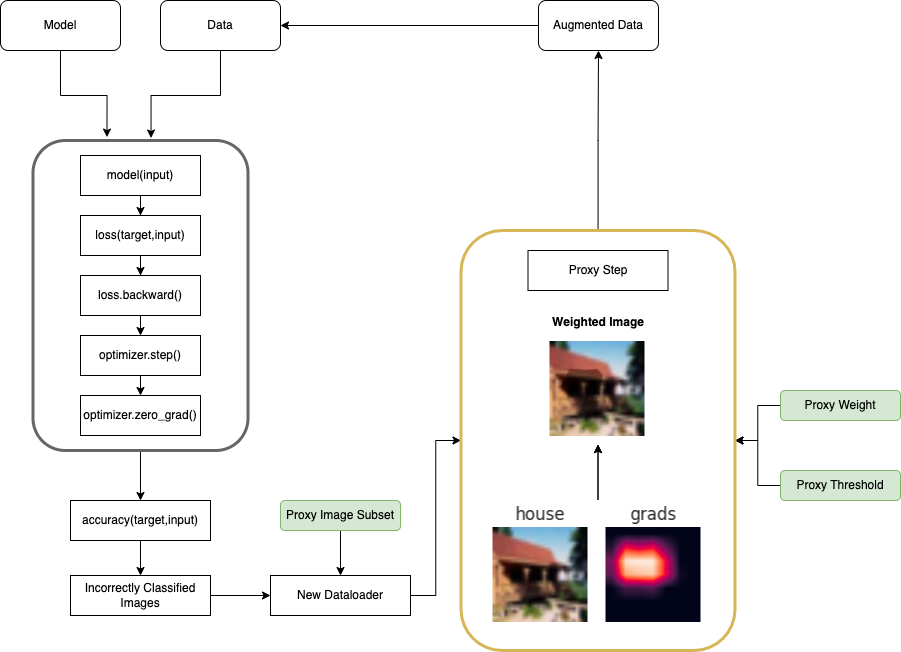
\includegraphics[width=.8\textwidth]{images/proxy_flow.png}
    \caption{Proxy Attention Visualized}
    \label{fig:proxy_flow}
\end{figure}

\section{Implementation}
This section describes the implementation of Proxy Attention in detail. 
\subsection{Hyper Parameters} \label{sec:hyperparameters}
Proxy Attention is a novel method, and so there is no previous research on the best hyperparameters to use. The objective in choosing them is to find a balance between performance, computational overhead, and memory usage. The following section discusses the different hyperparameters that were tested and the reasoning behind their selection.

\subsubsection{Proxy Method}
The Proxy Attention step involves replacing the pixels in the original images based on the attention maps obtained from a trained model. There are many different ways in which this can be done, some that were explored in the literature, some that were implemented and others that were left for future research. The following are the different methods that were considered:

\textbf{Image Statistics Based Replacement}

These methods use local or global statistical information from the images for replacement. All these methods can be computed per image, batch, or entire dataset.

\begin{enumerate}
    \item \textbf{Average Pixel Value}: The average pixel value of the original image is used for replacement.
    \item \textbf{Max Pixel Value}: The maximum pixel value of the original image is used for replacement.
    \item \textbf{Min Pixel Value}: The minimum pixel value of the original image is used for replacement.
    \item \textbf{0/255 Pixel Value}: The pixel value of 0 or 255 is used for replacement, where 0 refers to black and 255 refers to white.
\end{enumerate}
These methods are simple but naive, leading to significant information loss. In many cases, if many images have their values replaced with these values, the model might become biased towards predicting a specific class when an image contains many pixels with these values.
Due to this reason, these methods were not considered for the final implementation. A visualization of these methods can be found in Figure ~\ref{fig:methods}.

\textbf{Data Augmentation Based Replacement}

Data Augmentation techniques involve computing some transformation over images. Many of these methods were covered in the literature survey (Section ~\ref{sec:augmentation}), some of which replaced the pixels with random values, pixels sampled from either the current image or another image in the dataset, or even deleted the pixels. Most of these methods do not consider the model itself, but some, such as Saliency Mix \cite{uddinSaliencyMixSaliencyGuided2021} use saliency measures to find patches from other images in the dataset that are used to replace the chosen pixels.
These methods inspired Proxy Attention, but instead of replacing image patches or deleting pixels, it uses a gradient-based method to down-weight the pixels that might have led to the wrong prediction. This method moves away from using naive statistical information but enables the model to learn from its mistakes eventually.

% \subsubsection{\textcolor{red}{GAN Based Replacement}}


\textbf{Modifying the Weights}

Instead of replacing the pixels, another possible method would be to modify the network weights directly. While many research papers elaborate on methods to perform this procedure, this domain still needs to be researched enough to be used easily. Research on this domain has been done from the early 90s \cite{schmidhuberSelfReferentialWeightMatrix1993}, but practical implementation of such a network that learns to modify its weight while training has not been extremely successful \cite{irieModernSelfReferentialWeight2022}. 

Another such attempt to create a network closely inspired by the neuron plasticity of the human brain was done by Miconi et al. in their paper \cite{miconiBackpropamineTrainingSelfmodifying2020}. In human brains, the learning and forgetting is controlled by plasticity, the ability of the brain to modify it's previous understanding of concepts and solidify or remove these concepts if necessary. With this theme, Miconi et al. perform research emulating these functions used neuromodulated LSTMs that were given the ability to not only use gradient decent to optimize the weight themselves, but the plasticity of the weights as well. The authors find that these networks outperform standard LSTMs by a significant margin given an LM task, thus creating their training pardigm Backpropamine. Backpropamine is given a neuromodulated signal that controls the plasticity. In the brain, the chemical dopamine also potentially affects the synaptic weights, and thus Backpropamine is also affected by a decaying change in the weights given the right conditions.

While these methods do work, they are quite challenging and rely on very different types of networks than those that are usually used in CV research. That being the case, implementing such a method is left to future research.

\textbf{Multiply with Attention Map}

The method chosen for this research does not directly replace the image's pixels but weights them using the attention map generated by passing the image through the trained model.
The obtained attention map is thus multiplied with the original image. In line with the principles of Proxy Attention, this allows the network to understand that the parts of the image it initially focused on did not lead to the correct result. Note that doing so is only possible if the network has seen this image. Because the images are slightly modified after the Proxy Attention step, if the network still needs to learn what the original image looks like, it might make more mistakes in the future by learning the wrong set of features.

A caveat of this method is that, after successfully applying the Proxy step to an image, the number of weighted pixels increases and, over time, might lead to the image not having any useful features left. This loss of information is tackled by clearing the proxy images every couple of steps.
A visualization of this method compared to others can be found in Figure ~\ref{fig:methods}.

\begin{figure}[h]
    \centering
    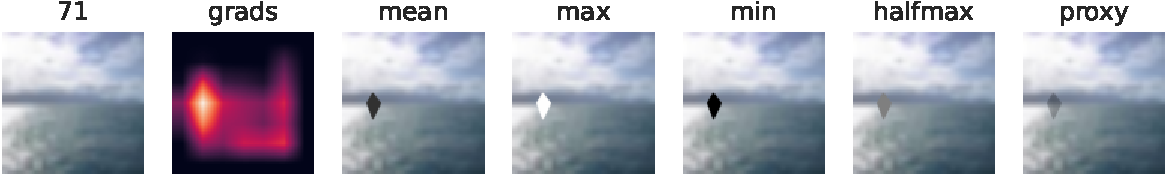
\includegraphics[width=1\textwidth]{images/methods-crop.pdf}
    \caption{A comparison of different methods to replace the pixels in the original image}
    \label{fig:methods}
\end{figure}

\subsubsection{Gradient Method}
Many gradient-based methods are available for generating attention maps from trained networks. While many of these methods were mentioned in the survey, it was impossible to test them all. Since Proxy Attention's effectiveness depends quite a bit on the gradient method used, it was important to test them.

The important factor considered while choosing these methods was the difference in complexity and the power of explanation they provide. While algorithms like GradCAM++ \cite{chattopadhayGradCAMGeneralizedGradientBased2018} provide more nuanced and better explanations of the image, older algorithms like Vanilla Gradients \cite{zeilerVisualizingUnderstandingConvolutional2013} are not so accurate. The objective here was to understand if using a more powerful method would improve performance with respect to classification accuracy when used with Proxy Attention. If this is the case, then it is possible to use more powerful methods to further improve performance in the future.
The gradient methods that were tested are as follows:
\begin{itemize}
    \item \textbf{GradCAM++} \cite{chattopadhayGradCAMGeneralizedGradientBased2018}.
    % \item \textbf{GradCAM} \cite{selvarajuGradCAMVisualExplanations}
    \item \textbf{EigenGradCAM} \cite{banymuhammadEigenCAMVisualExplanations2021}
\end{itemize}
For further explanations, refer to the literature survey in Section ~\ref{sec:gradient_based_explanations}.

\subsubsection{Gradient Threshold (Proxy Image Threshold)}
Every gradient method considered generates a heatmap where the higher the activation, the more important the pixel is. The activations are mapped to a $[0,1]$ range with higher values in the heatmap indicating higher activation values. Since using Proxy Attention would mean that the pixels with the chosen activation values would be down-weighted, choosing a threshold value would result in the best classification accuracy was important.\\
This is a balancing act as choosing too small of a threshold would result in larger parts of the image being down-weighted, while choosing too large of a threshold would result in the image being down-weighted too little and hence being too close to the original image to make any difference.\\
A visualization of the different thresholds and their effects is shown in Figure \ref{fig:thresholds_and_mults}.

\subsubsection{Multiply Weight (Proxy Image Weight)}
The Multiply Weight hyperparameter is used to control how strongly the attention map is applied to the image. The values are in the range $[0,1]$. A higher value would mean that the image is more strongly affected by the attention map, while a lower value would mean that the image is less affected. This is a balancing act as choosing too high of a value would mean that the image is affected too much, and important features might be lost from the image. Choosing too low of a value would mean that the image is not affected enough, rendering the Proxy step useless. The optimal value of this hyperparameter is found based on the results of the experiments conducted. A visualization of the different multiply weights tested is shown in Figure \ref{fig:thresholds_and_mults}.

\begin{figure}[!htb]
    \begin{subfigure}[b]{0.5\textwidth}
        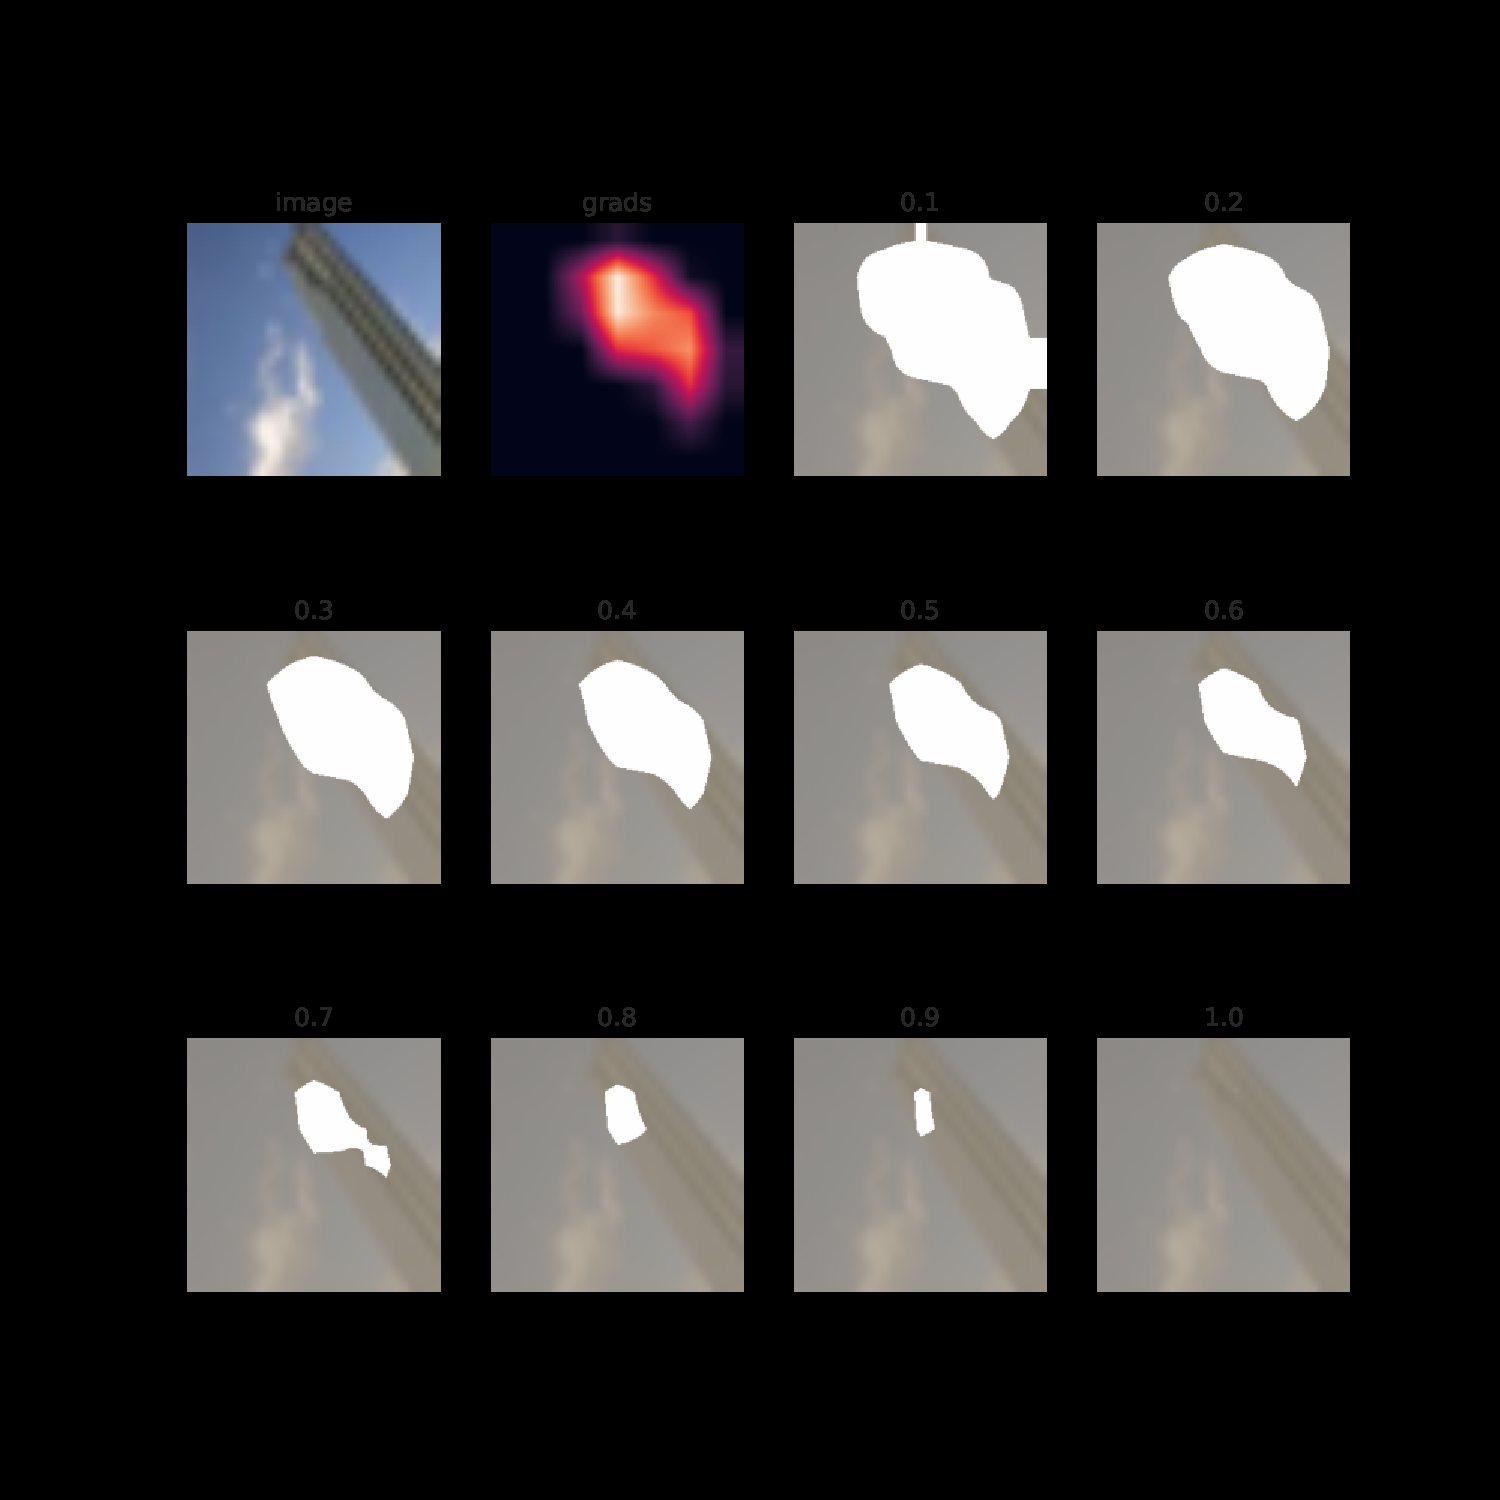
\includegraphics[width=\linewidth, right]{images/grad_threshold.pdf}
        \caption{A visualization of the different thresholds and their effect on the image}
        \label{fig:thresholds}
    \end{subfigure}
    % \hfill
    \begin{subfigure}[b]{0.5\textwidth}
        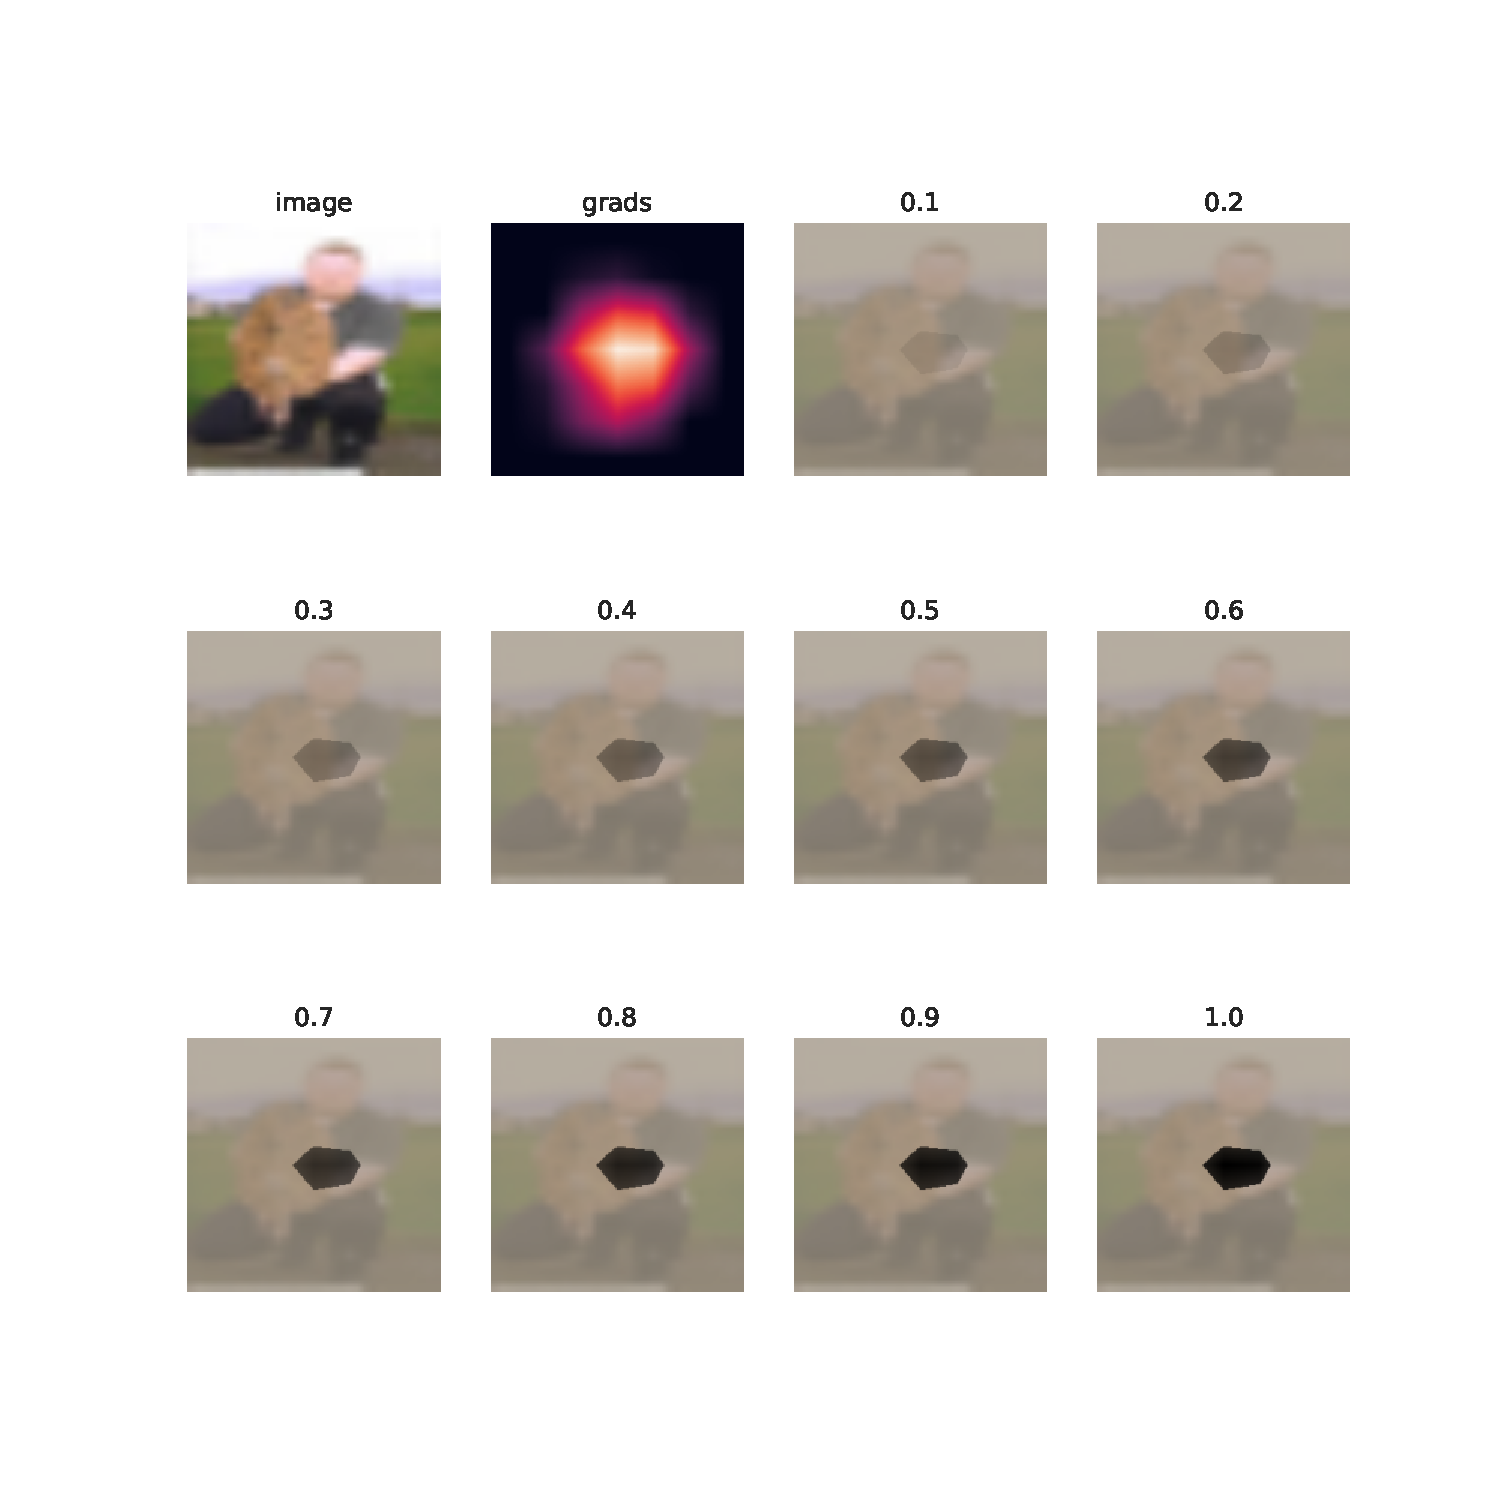
\includegraphics[width=\linewidth, left]{images/multiply_threshold.pdf}
        \caption{A visualization of the different multiply weights and their effect on the image for a Gradient Threshold of 0.8}
        \label{fig:mults}
    \end{subfigure}
    \caption{A visualization of the different thresholds and their effect on the image}
    \label{fig:thresholds_and_mults}
\end{figure}

\subsubsection{Proxy Step Schedule}
Proxy Attention is a novel method, which means that there was no previous literature on how often to apply the Proxy step. To test this, multiple schedules were tested to understand how the network performs when the Proxy step is applied at different times.\\
The challenge faced while testing for this was that if the Proxy step was applied too many times, it might lead to overfitting, while if it was applied too few times, it might not have any effect. One might consider applying the Proxy step for every step, but this would be too computationally expensive. Since Proxy Attention also relies on the understanding of the model, applying the Proxy step too many times initially, when the network is not trained yet, might degrade performance as well.\\
These issues indicate a need for a schedule for the Proxy step as well. It is manually scheduled as of now, except when using the schedule generator (which is also a naive method).\\
Future work might include generating a schedule with respect to the validation accuracy. This might be a good idea as, if the network is not learning well, the Proxy step could be applied more often. But if the performance is already sufficient, then there remains no need to apply the Proxy step as frequently and potentially degrade performance.


\subsubsection{Subset Of Wrongly Classified Images}
This hyperparameter was chosen to understand if increasing the number of images that are passed to the Proxy step would help in improving performance. While providing more images might lead to better performance, the more images that are passed to the Proxy step, the more computationally expensive it becomes. To test this, both ends of the spectrum were tested, with a small fraction and a large fraction of the images being passed through the Proxy step.\\
As of now, the number of images passed to the Proxy step is taken as a fraction of the total number of images in the dataset. Future work could include a schedule for this as well, where the number of images passed to the Proxy step decreases over time as the network learns more and does not need as much help in improving performance.

\subsection{Training Biases}
Gradient-based XAI methods are not perfect, and in many cases, they are unable to provide accurate explanations for the predictions made by the model. Since Proxy Attention relies on the outputs of these methods, this might lead to the model learning biased representations of the data. This section discusses the different biases that might be introduced by using these methods in combination with Proxy Attention and how they can potentially be mitigated.

\textbf{Method Bias}

Not all explainability methods perform equally. Some methods are shown to have better masks generated, while other methods are more computationally expensive. Since Proxy Attention heavily depends on these methods, using them may lead to additional artefacts in the generated images. Some methods lead to better results while being used alongside Proxy Attention. To test the effects of this, multiple gradient-based methods are used to compare the performance of the networks.

\textbf{Mask Bias}

Proxy Attention uses the attention maps produced by gradient-based methods and multiplies them on the original image as a mask. While this works well, the masks themselves have edge artefacts that may lead to corrupting some regions of the image. These artefacts are further amplified for smaller image sizes and might impact performance in the long run.
Potential solutions include:

\begin{enumerate}
    \item Smoothing the masks before applying them to the image using techniques such as Eigen Smoothing. This could help in reducing the edge artefacts.
    \item Ensuring that only a certain percentage of the image is replaced by the Proxy Attention step. Doing so would preserve more information.
\end{enumerate}

\textbf{Learning Bias}
\begin{enumerate}
    \item Testing multiple schedules of when to apply the Proxy Attention step. This would help in understanding which part of the training process would benefit from the Proxy Attention step the most, reducing the computational overhead in the long run.
    \item Not reusing previously masked images for the Proxy Step. Doing so ensures that the artefacts are not propagated further into the training process.
\end{enumerate}

\subsection{Overview of the Codebase}
This section provides an overview of the code structure and the datasets used in this project. The code is written in Python 3.10.10 , and uses PyTorch version 2.0.0. The entire codebase is available on \href{https://github.com/SubhadityaMukherjee/proxy_attention}{GitHub}. (As of now, the code is private, but will be made public after the evaluation is complete.) The entire requirements are listed in the \textit{requirements.txt} file in the root directory of the codebase. The structure of the codebase is shown in Figure ~\ref{fig:overview_code}.
A separate directory is used for each dataset, with each dataset being split into training and testing subdirectories. The results directory contains the aggregated runs, which are used directly in the report. The figures and tables are generated from the aggregated runs using the \textit{log\_viewer.ipynb} file. The runs directory contains the runs of the model. Each run has a folder with the run number, which contains the tensorboard logs and the checkpoints. 
The \textit{src} directory contains the source code for this project. The \textit{main.py} file is the entry point for the code and is used to configure the runtime hyperparameters. The \textit{proxyattention} folder contains the code for the model and the \textit{meta\_utils.py} file contains utilities that are reused across the codebase while the \textit{training.py} file contains all the code required for Proxy Attention and training the models.

\begin{figure}[!htb]
    \centering
    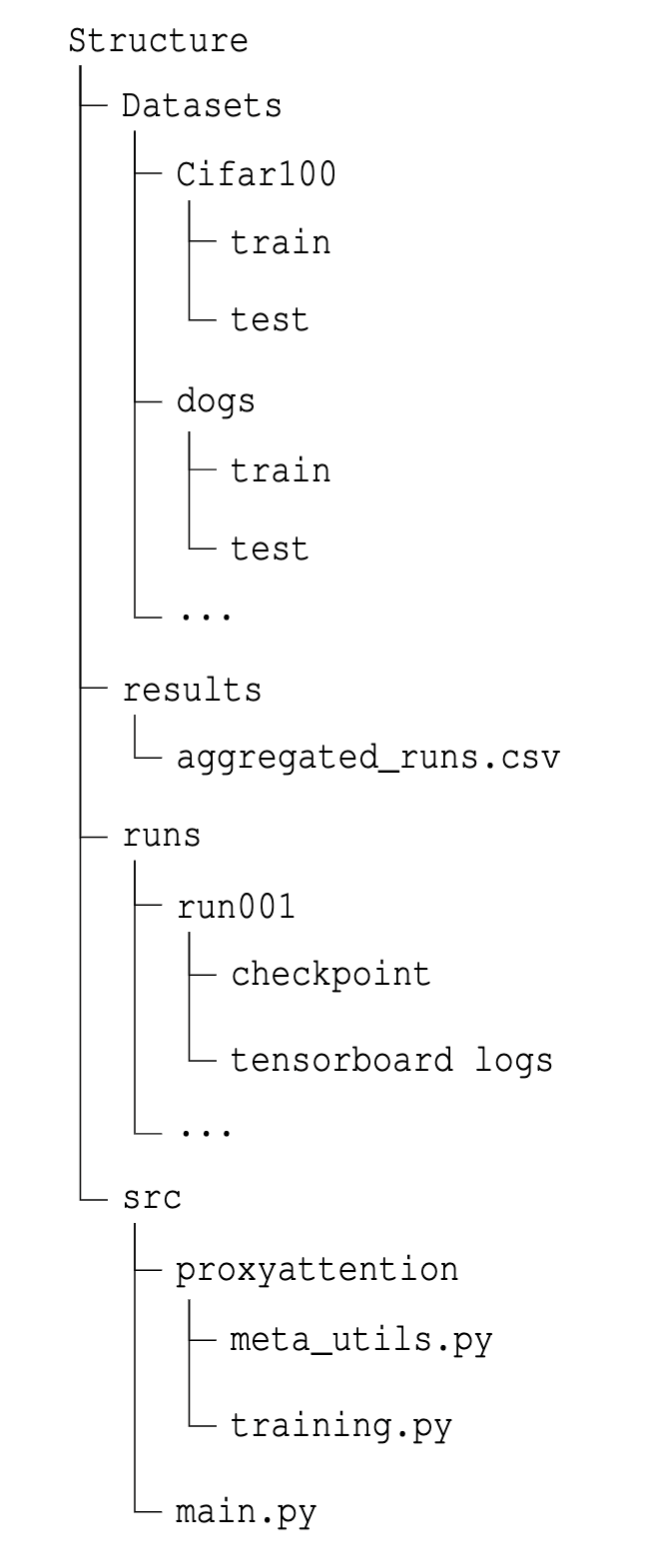
\includegraphics[width=.3\linewidth]{images/dirstruct.png}
    \caption{Code Directory Structure}
    \label{fig:overview_code}
\end{figure}


\subsection{Datasets}
To test Proxy Attention, a variety of datasets were chosen. The datasets were chosen to be of varying difficulty, and to have varying number of classes. The datasets used are \textbf{CIFAR100, Stanford Dogs, ASL Alphabet and Plant Disease dataset}. The datasets are described in detail in the following sections.

The images provided by the datasets are of varying sizes, but are resized to a similar size for consistency. These visualizations were generated by the author, and are not fully representative of the original dataset but are provided for reference. Due to space constraints, not all classes are shown in the visualizations. The complete list of classes and examples can be found in the links provided.

\textbf{CIFAR 100}

The CIFAR 100 dataset, introduced by \cite{krizhevskyLearningMultipleLayers}, is an image dataset with 60000 colour images with dimensions 32x32 pixels. As the name suggests, the dataset has 100 unique classes. Each of these classes has 500 training images. Some classes are - \textbf{airplane, bird, truck, ship, deer and dog}. This dataset is used as a coarse-grained classification dataset in this project.\\
The dataset and complete class information can be found \href{https://www.kaggle.com/datasets/fedesoriano/cifar100}{here}.
A sample of the images from the dataset is shown in Figure ~\ref{fig:cifar100}.

\begin{figure}[!htb]
    \centering
    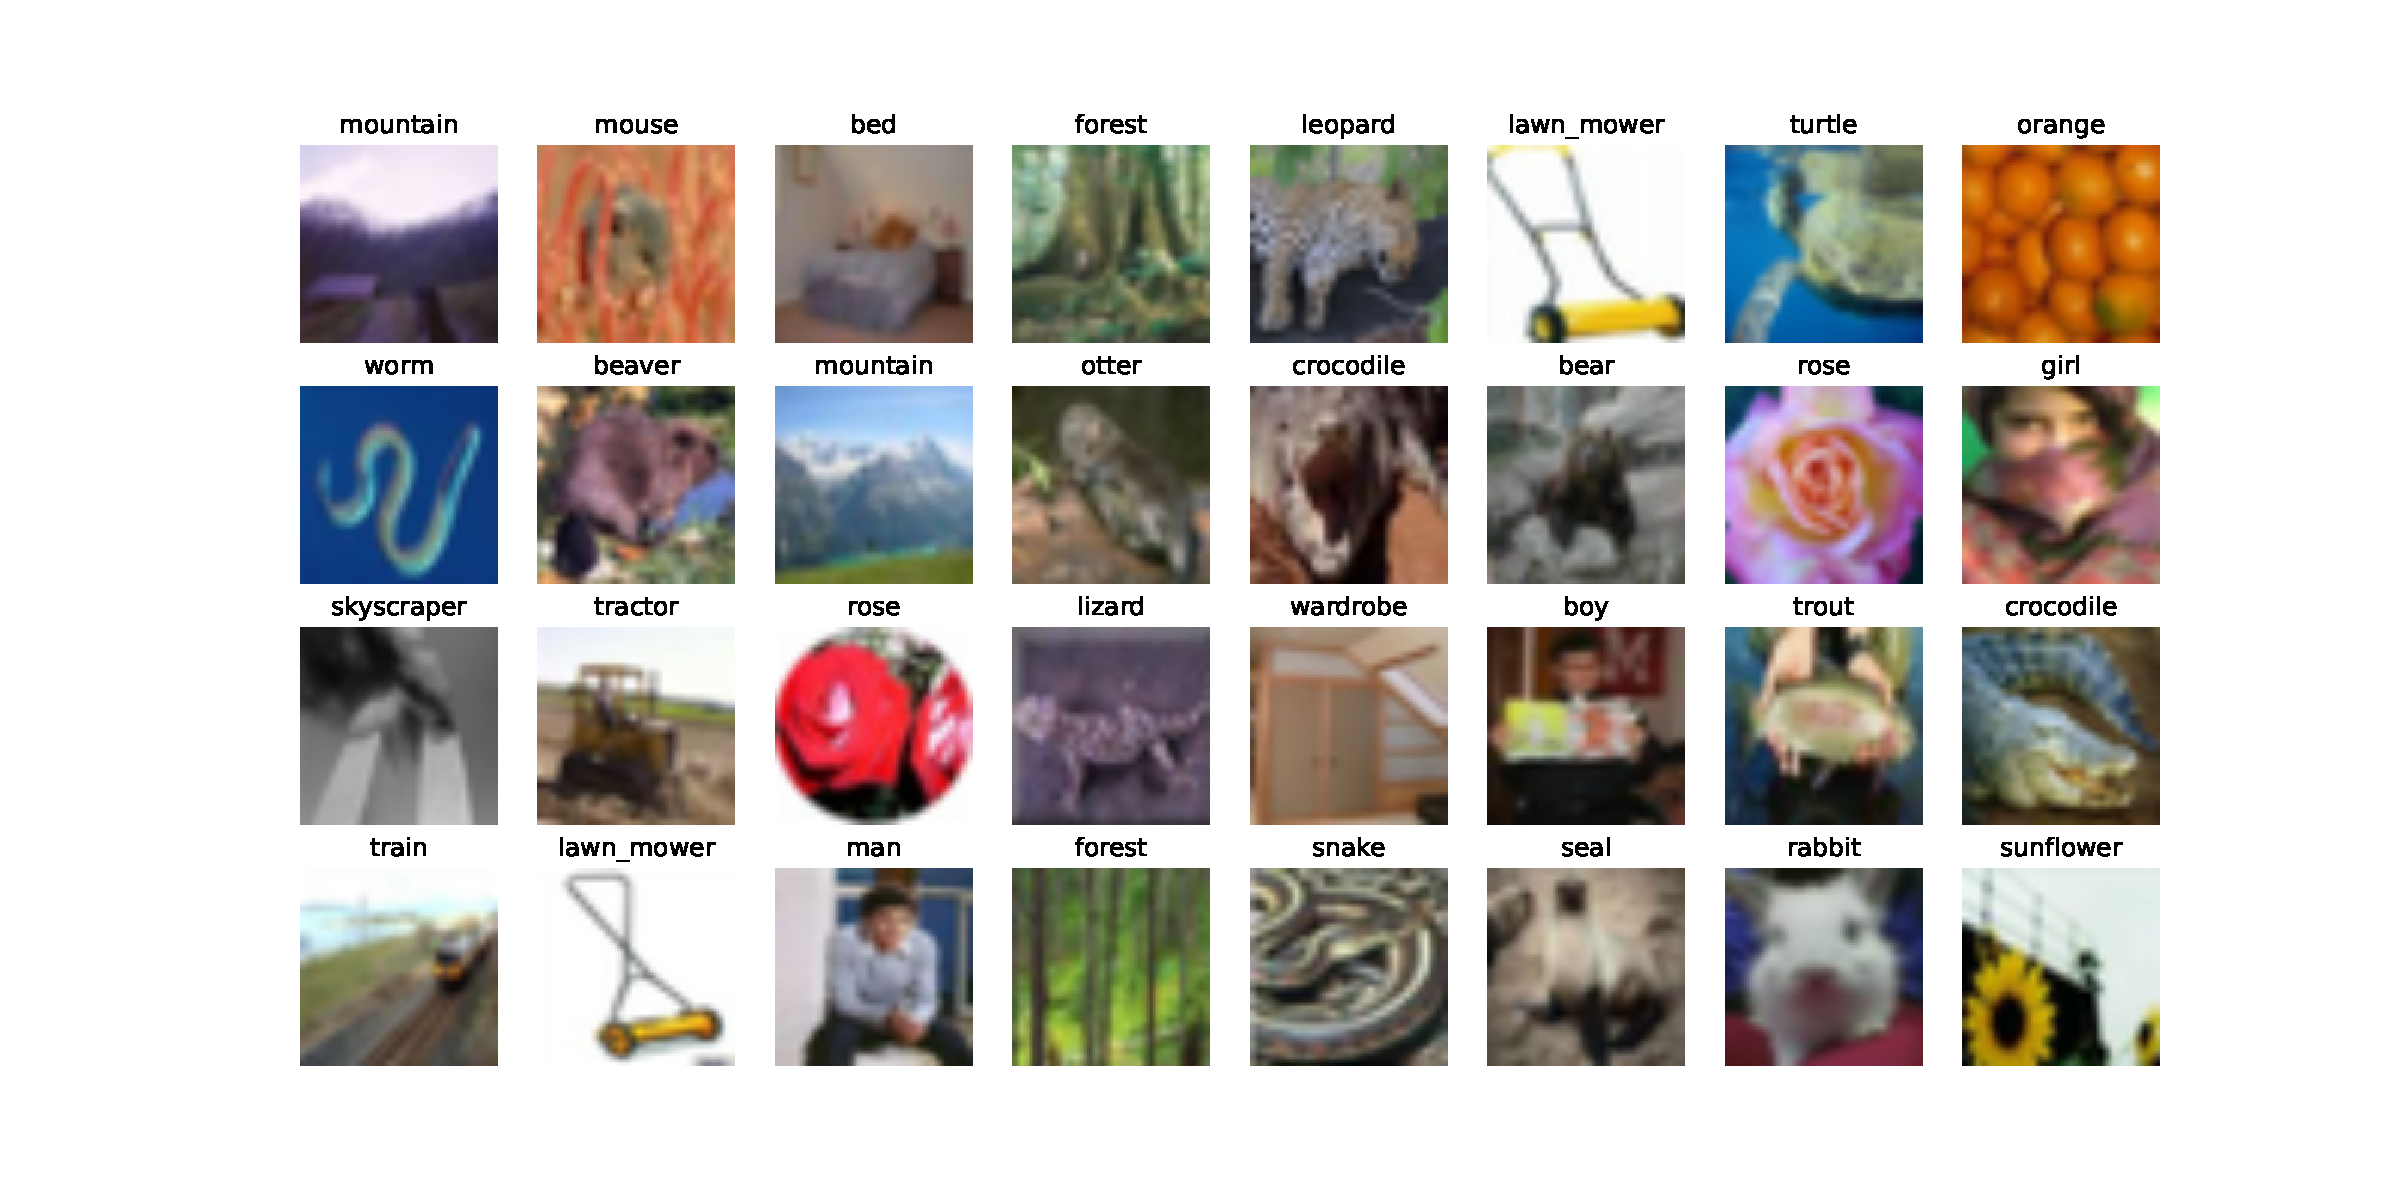
\includegraphics[width=1\textwidth]{images/cifar100.pdf}
    \caption{A batch of images from the CIFAR100 dataset}
    \label{fig:cifar100}
\end{figure}

\textbf{Stanford Dogs}

The Stanford Dogs dataset \cite{khoslaNovelDatasetFineGrained} is a popular fine-grained image classification dataset. There are more than 20k images in this dataset categorized into  120 classes of dog breeds like the \textbf{Afghan Hound , Appenzeller} etc. Being a fine-grained dataset, the images are very similar to each other and the classification task is much harder.\\
This dataset was chosen to further evaluate the explainability of Proxy Attention.\\
The dataset and complete class information can be found \href{http://vision.stanford.edu/aditya86/ImageNetDogs/}{here}.
A sample of the images from the dataset is shown in Figure ~\ref{fig:dogs}.
\begin{figure}[!htb]
    \centering
    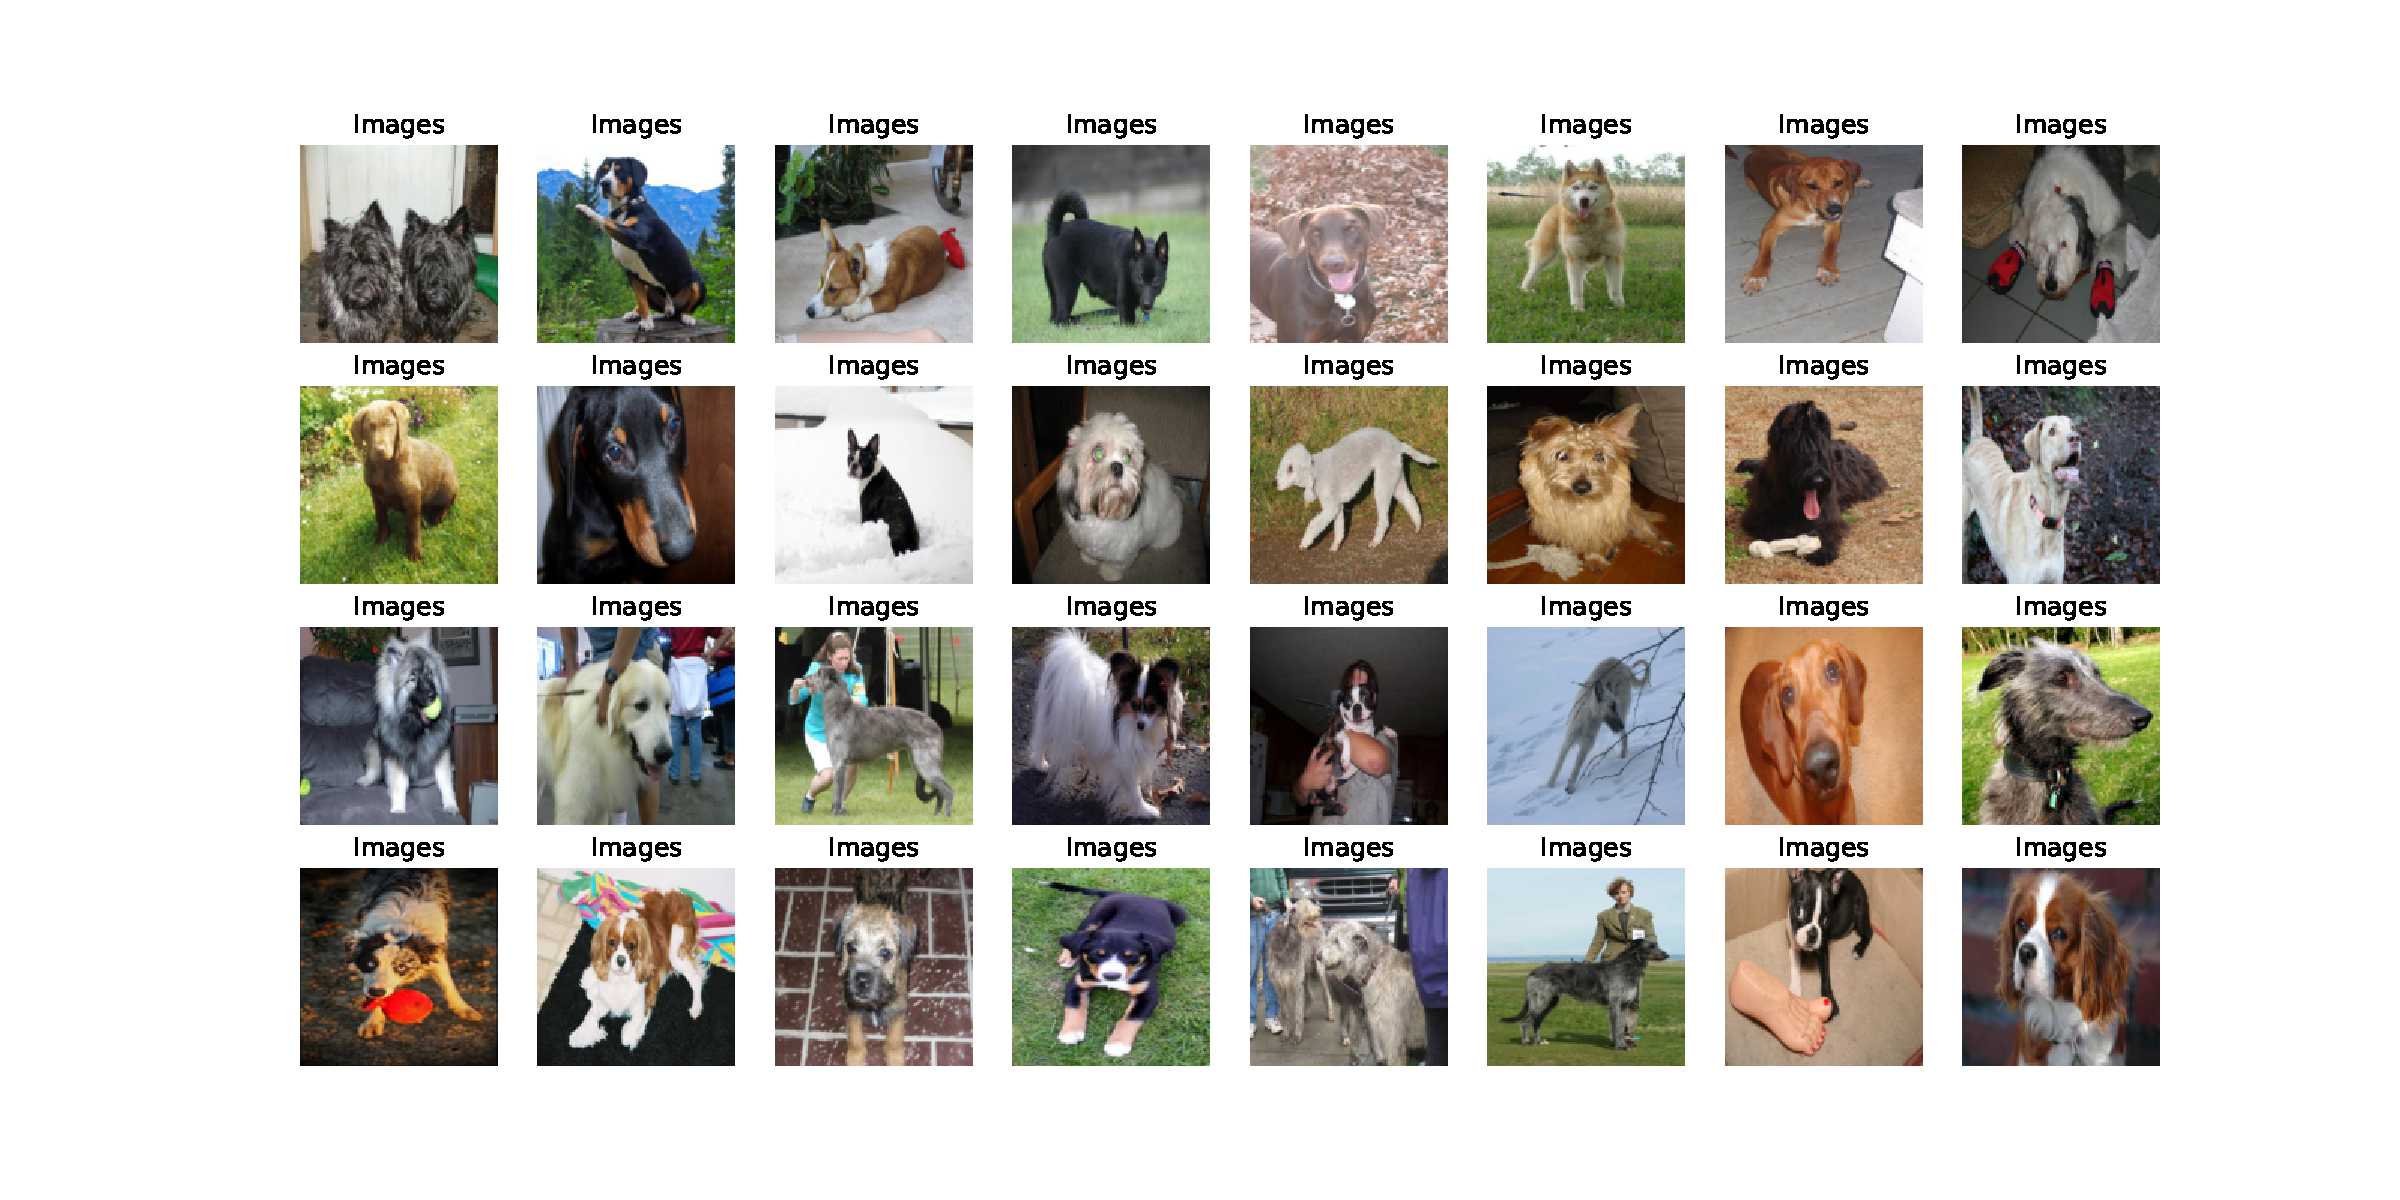
\includegraphics[width=1\textwidth]{images/dogs.pdf}
    \caption{A batch of images from the Stanford Dogs dataset}
    \label{fig:dogs}
\end{figure}

\textbf{ASL Alphabet}

The ASL dataset is a collection of hand pose images from the American Sign Language. There is no pose information with this dataset, but the images can be used for classification using the provided class labels.
The dataset chosen to evaluate Proxy Attention is the ASL Alphabet dataset, a more specific subset that has all the letters of the English alphabet along with the special characters \textbf{del, space and nothing}. The background is mostly the same, with minor changes. The data is also recorded from people with a similar skin tone, which makes the task easier.\\
This is an easy to classify dataset and was used as an initial test of the Proxy Attention mechanism. The results of the same are left in for future reference. \\
The dataset and complete class information can be found \href{https://www.kaggle.com/datasets/grassknoted/asl-alphabet}{here}.

A sample of the images from the dataset is shown in Figure ~\ref{fig:asl}.
\begin{figure}[!htb]
    \centering
    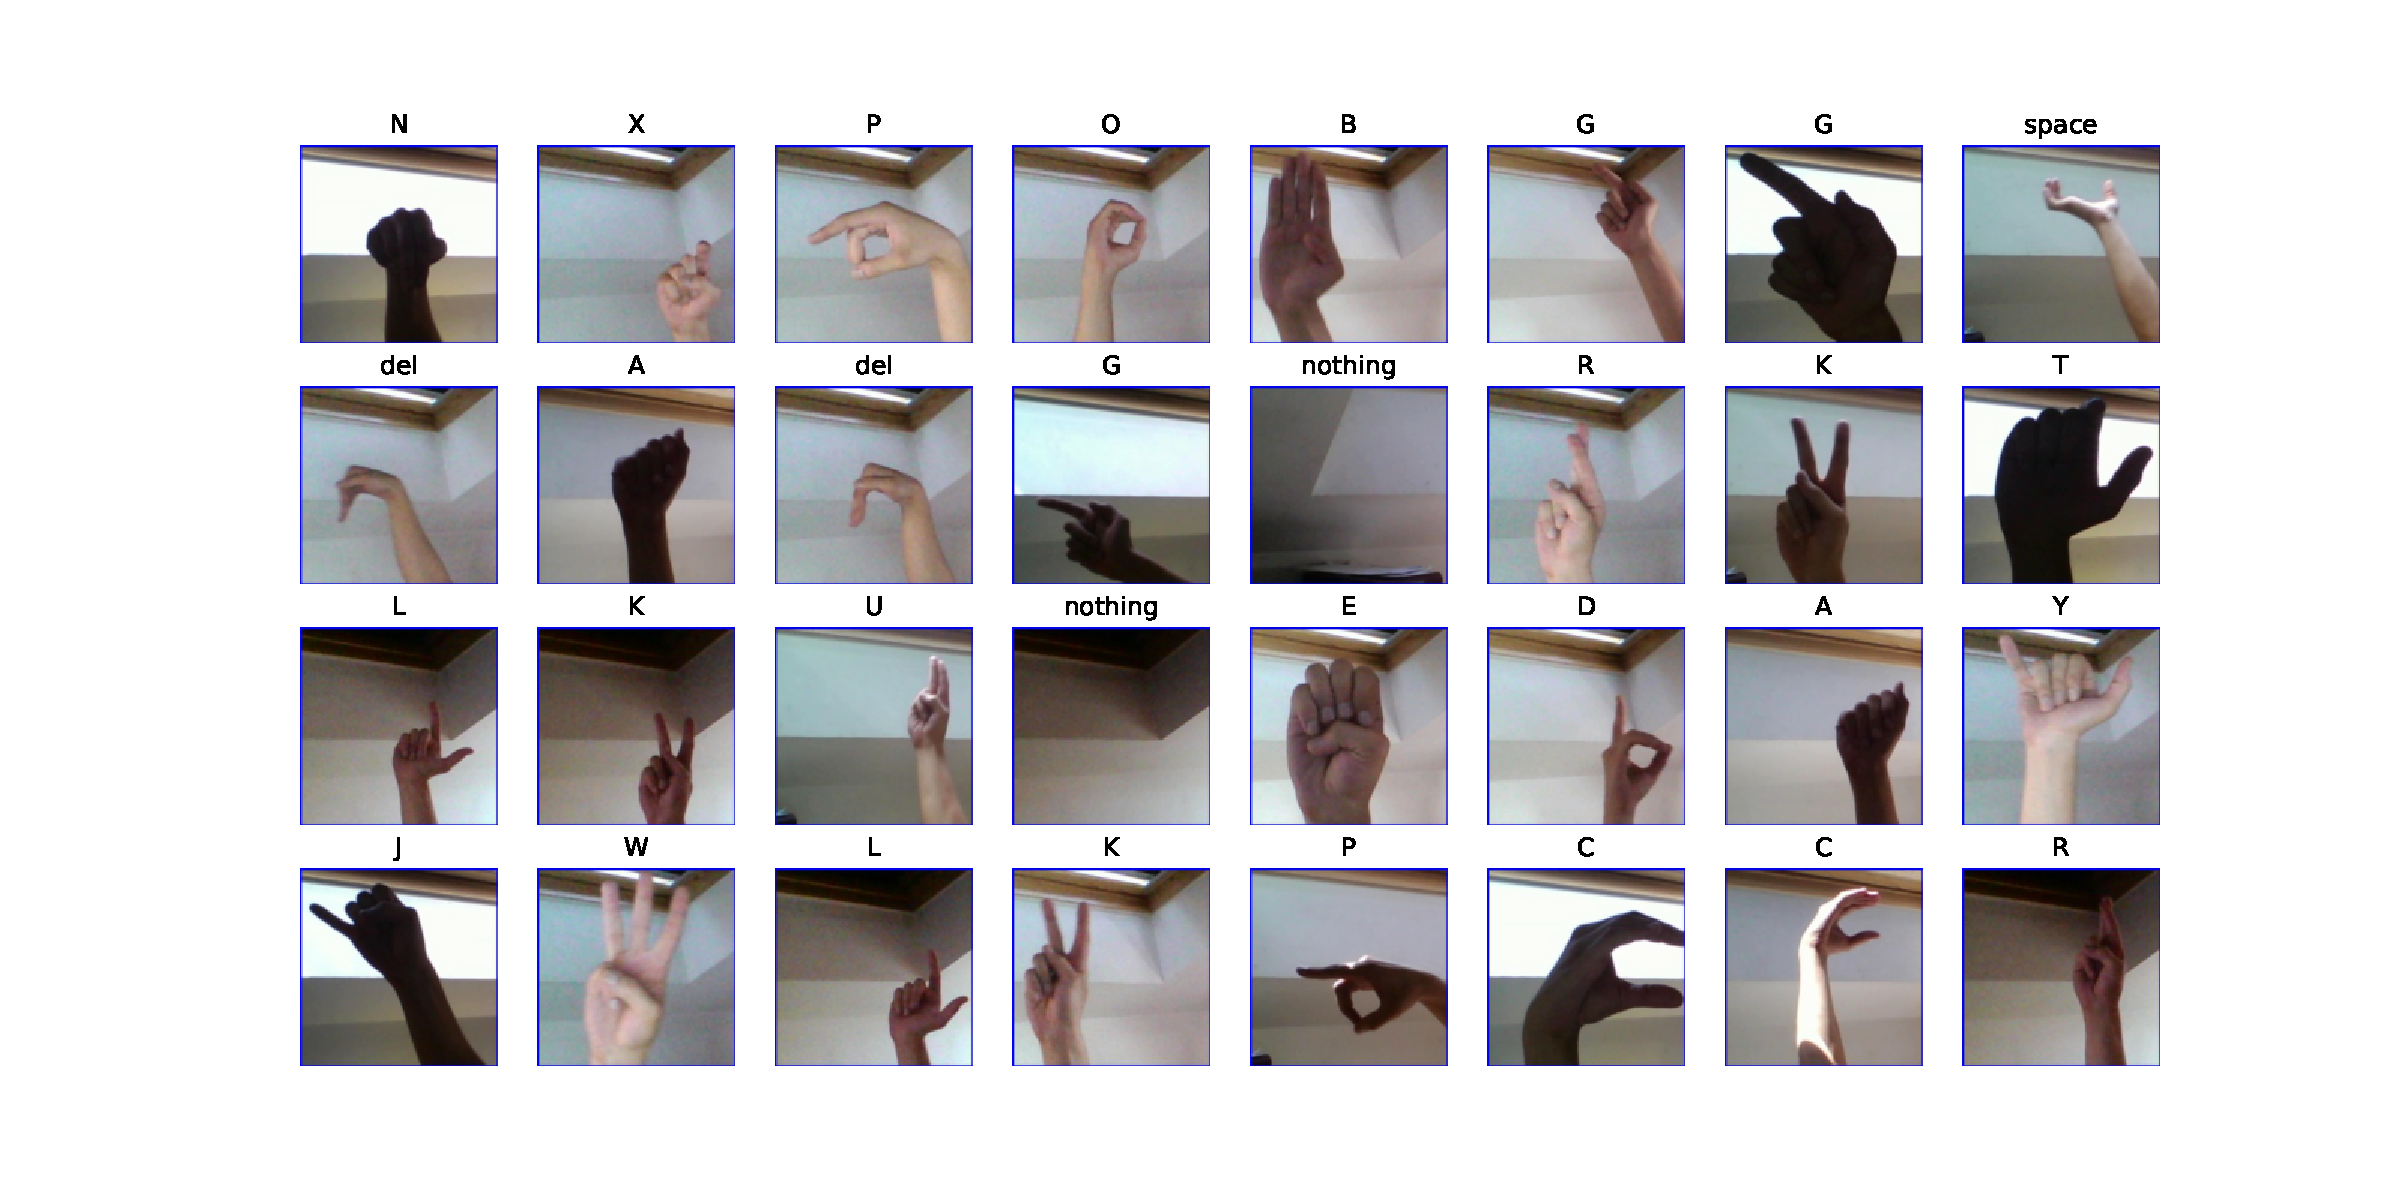
\includegraphics[width=1\textwidth]{images/asl.pdf}
    \caption{A batch of images from the ASL Alphabet dataset}
    \label{fig:asl}

\end{figure}

\textbf{Plant Disease}

This dataset consists of images of plant diseases across a variety of plants. The dataset is also a fine-grained classification dataset with 39 classes. Other than a few diseases, most of them are quite similar to each other, making the classification task harder. Some examples of the classes are \textbf{apple scab, blueberry healthy, cherry powdery mildew} etc.\\
The dataset and complete class information can be found \href{https://www.kaggle.com/datasets/rajibdpi/plant-disease-dataset}{here}.
\begin{figure}[!htb]
    \centering
    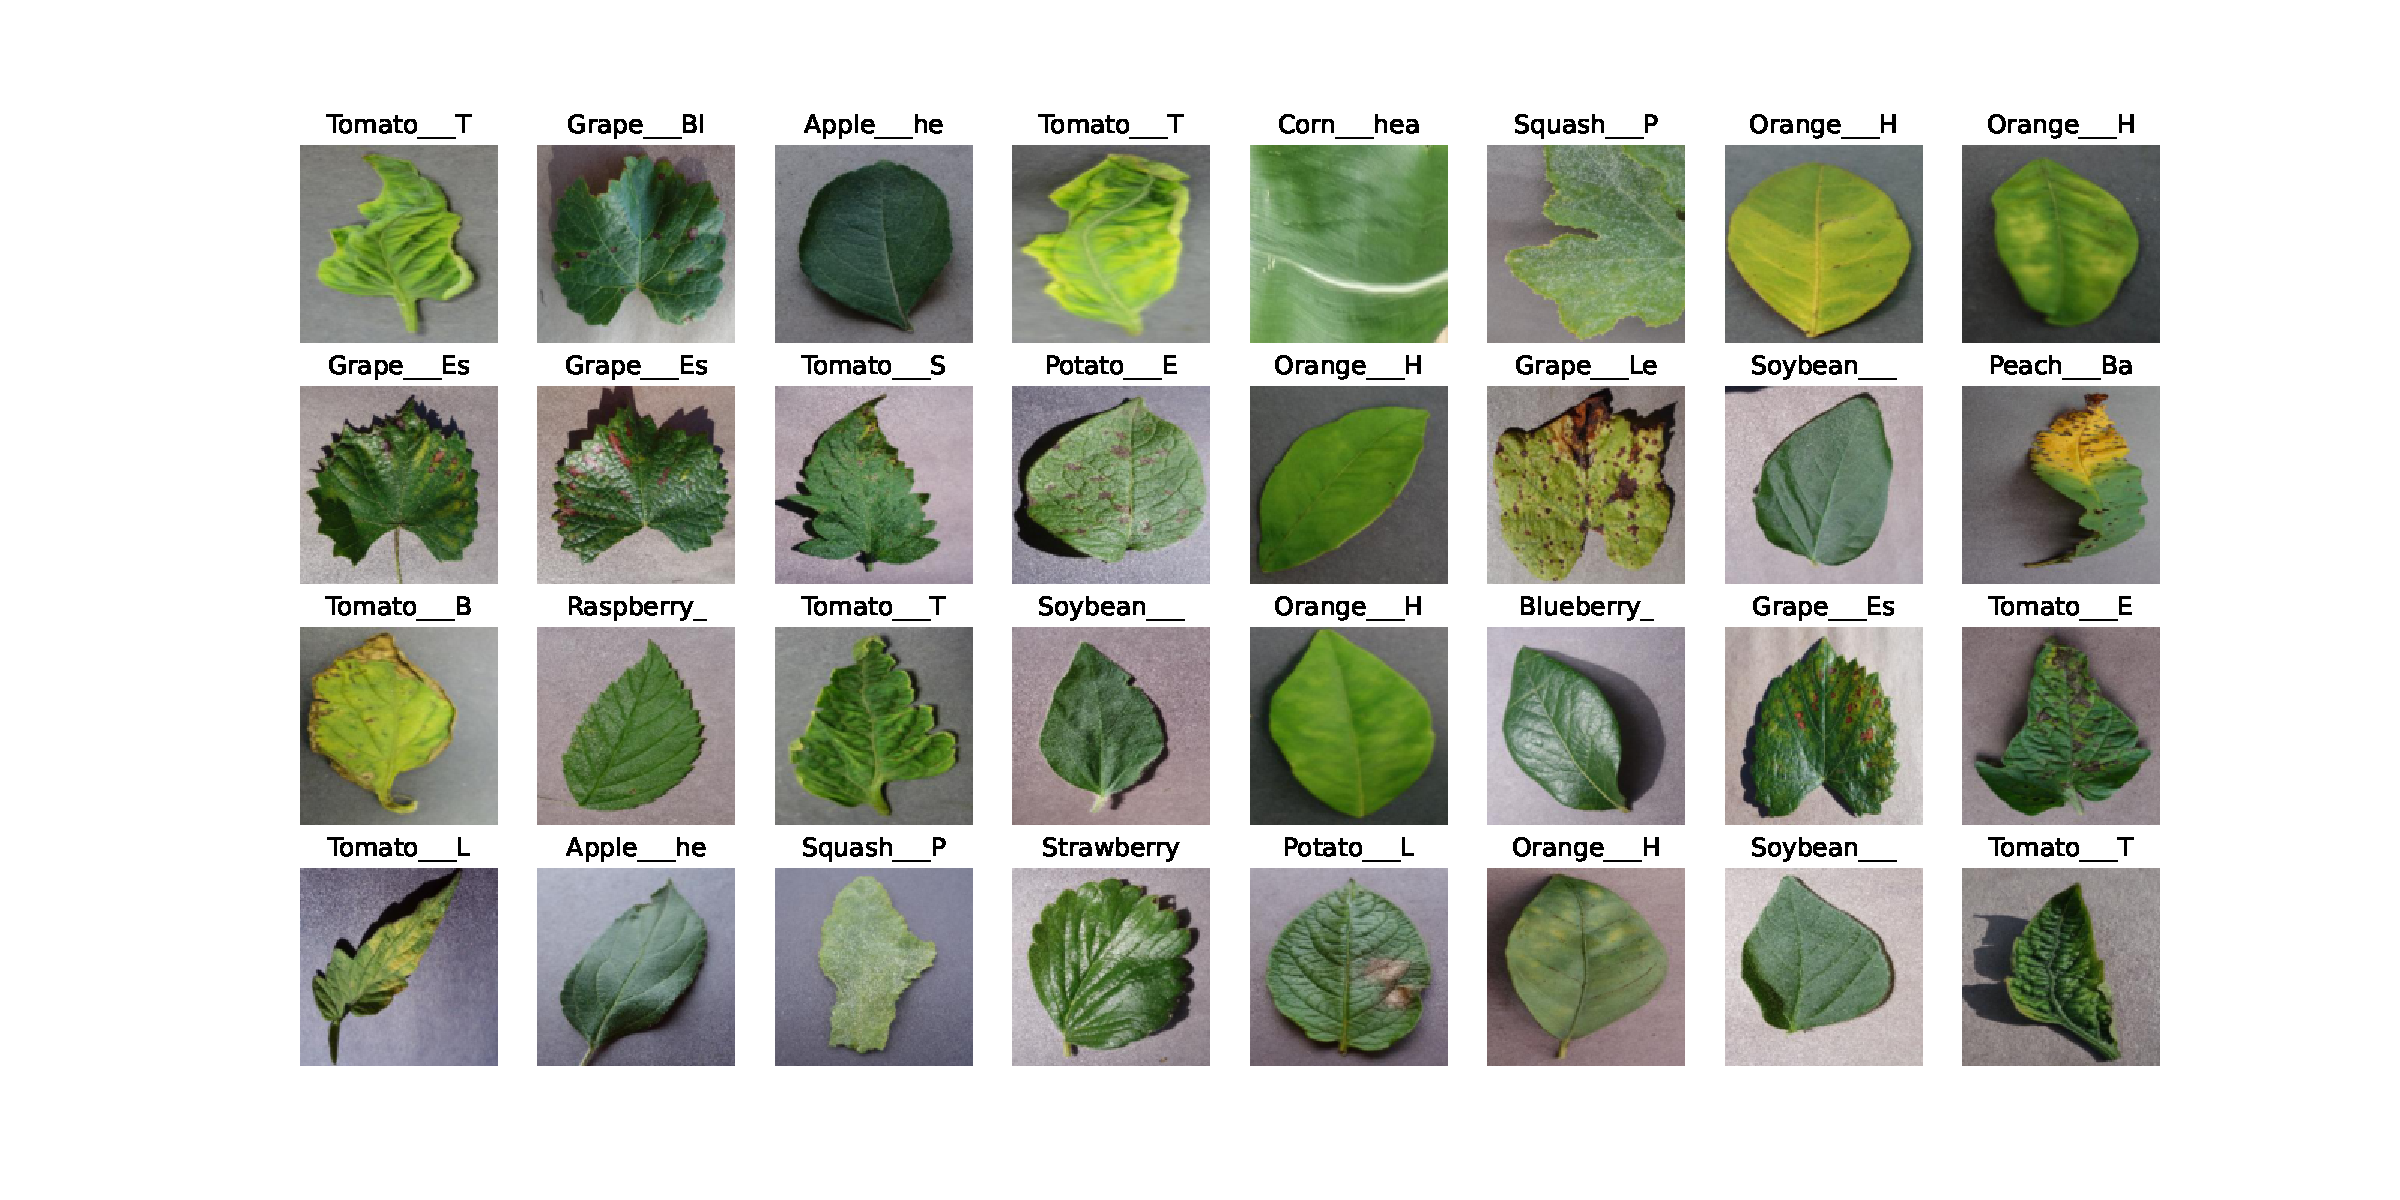
\includegraphics[width=1\textwidth]{images/plantdisease.pdf}
    \caption{A batch of images from the Plant Disease dataset}
    \label{fig:plant}

\end{figure}

\textbf{Caltech101}

The Caltech101 \cite{liCaltech101} dataset was created to tackle the absence of a uniform baseline comparison for vision classification tasks. The dataset has 101 categories of images, with a total of 9146 images. A background category is also included, which has images that do not belong to any of the 101 categories. An advantage of this dataset is that the images are of uniform size and have low clutter and occlusion, making it easier to classify. The caveat is that some categories have fewer samples than others.\\
The dataset and complete class information can be found \href{https://www.kaggle.com/datasets/862ae86edba271c39f76d0b530edeb55076b4b82b971160637210900747c44b1}{here}.

A sample of the images from the dataset is shown in Figure ~\ref{fig:calt}.

\begin{figure}[!htb]
    \centering
    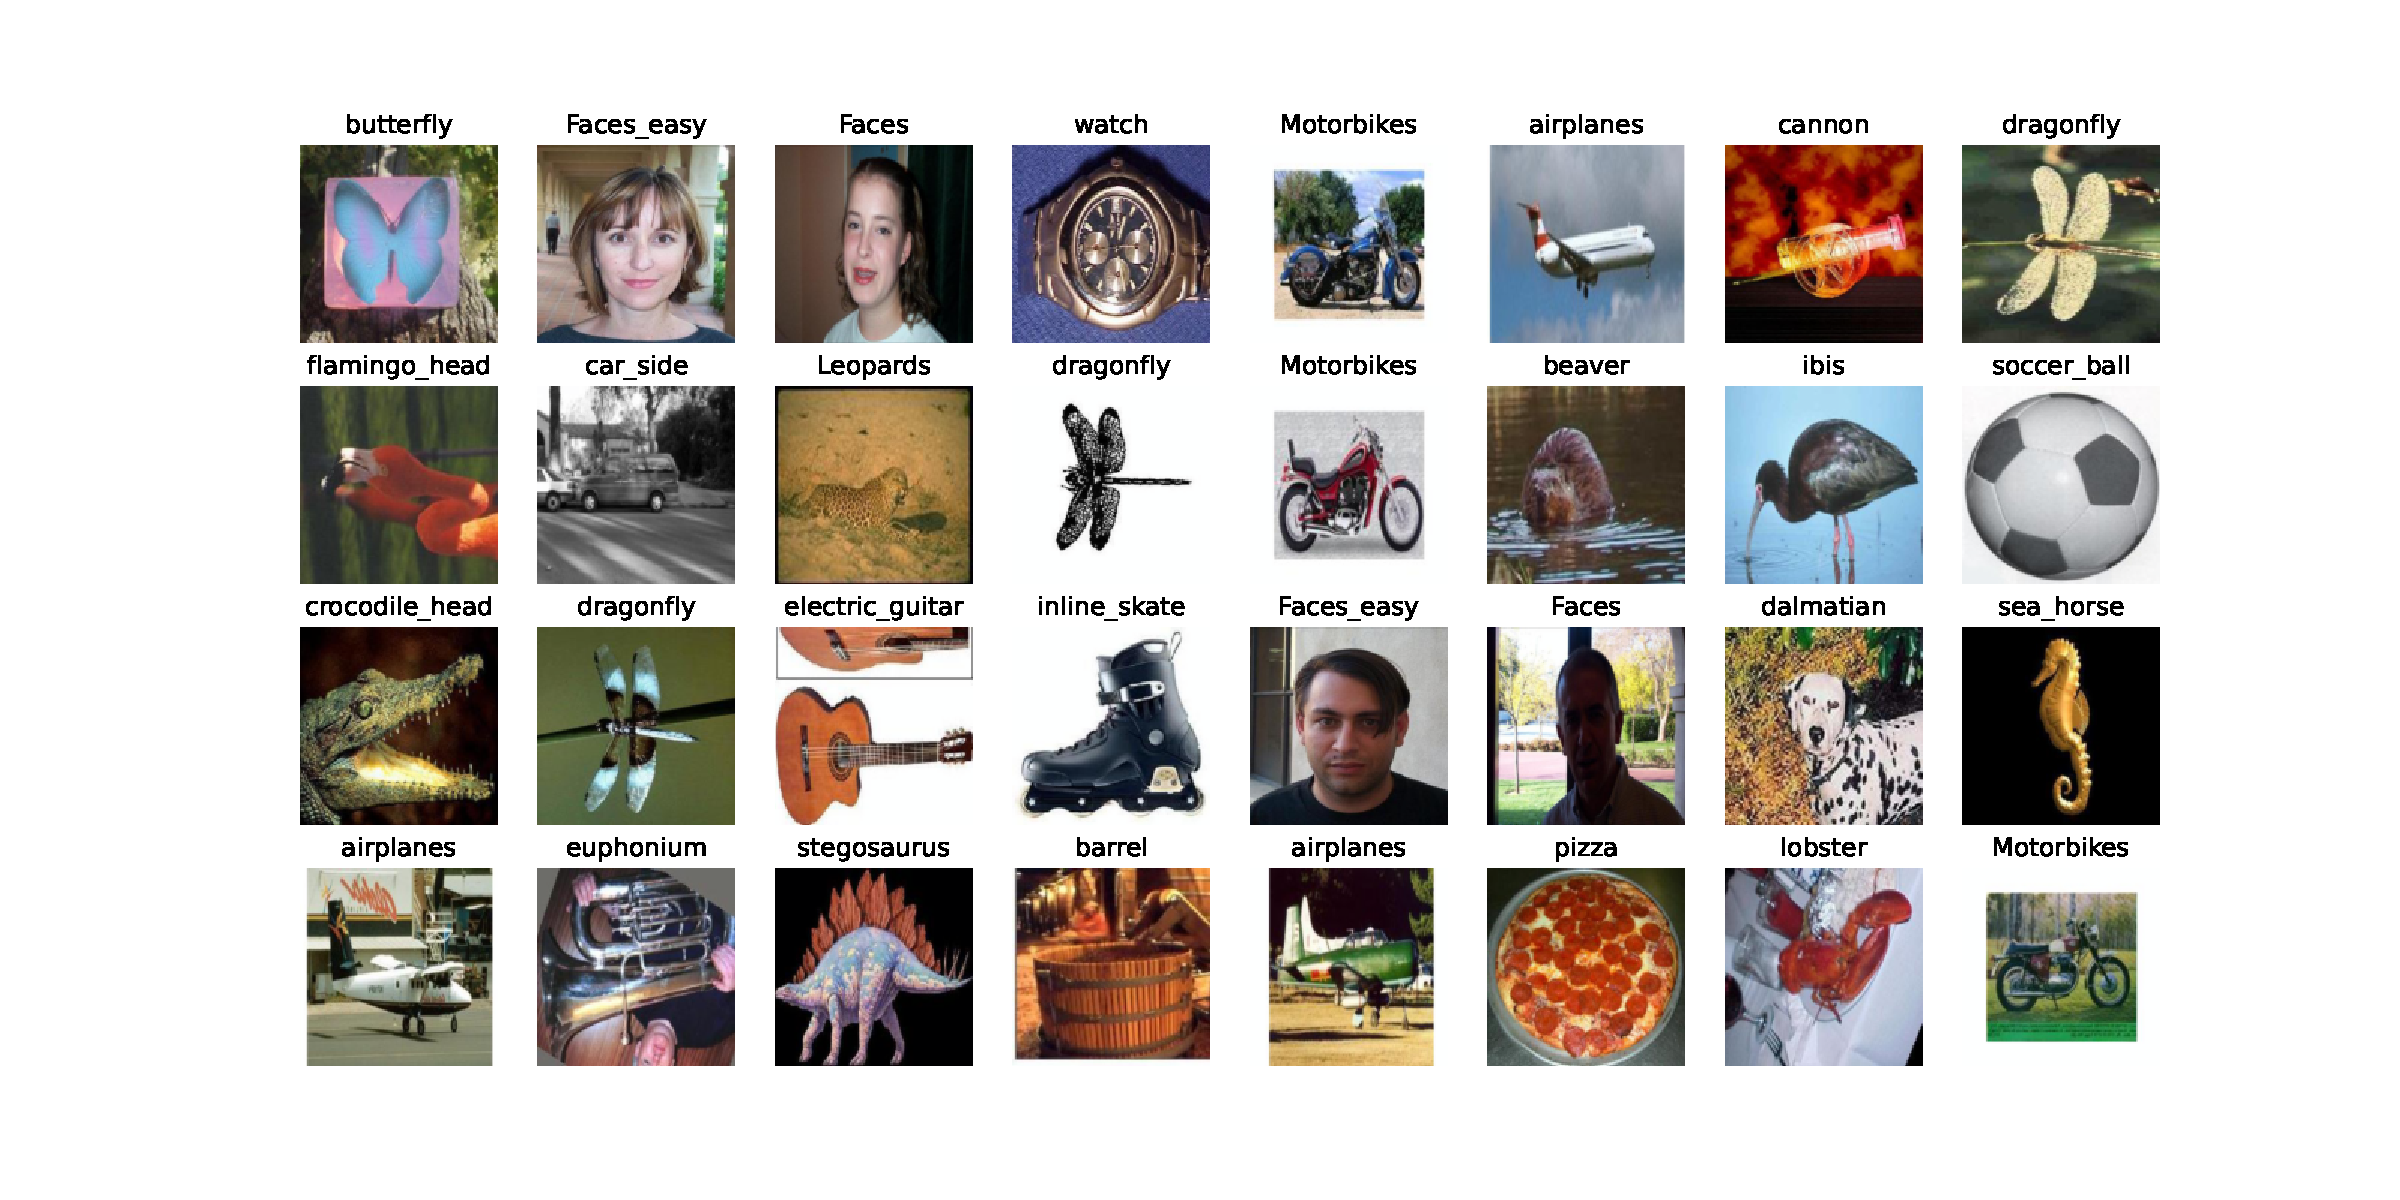
\includegraphics[width=1\textwidth]{images/caltech101.pdf}
    \caption{A batch of images from the Caltech101 dataset}
    \label{fig:calt}
\end{figure}

\textbf{Places}

The Places dataset \cite{zhouPlaces10Million2018} contains 2.5 million images of different scenes. These scenes contain both indoor and outdoor scenes and have been categorized into 205 classes, including engine room, excavation, and kitchen. This dataset used for this research is a subset of the MIT places dataset, which comprises a total of 10\% out of the original 10 million images. The large-scale nature of the dataset allows for extensive exploration of scene recognition and understanding tasks but here it is used as a coarse-grained image classification dataset.\\
The dataset and complete class information can be found \href{https://www.kaggle.com/datasets/mittalshubham/images256}{here}.

A sample of the images from the dataset is shown in Figure ~\ref{fig:places}.

\begin{figure}[!htb]
    \centering
    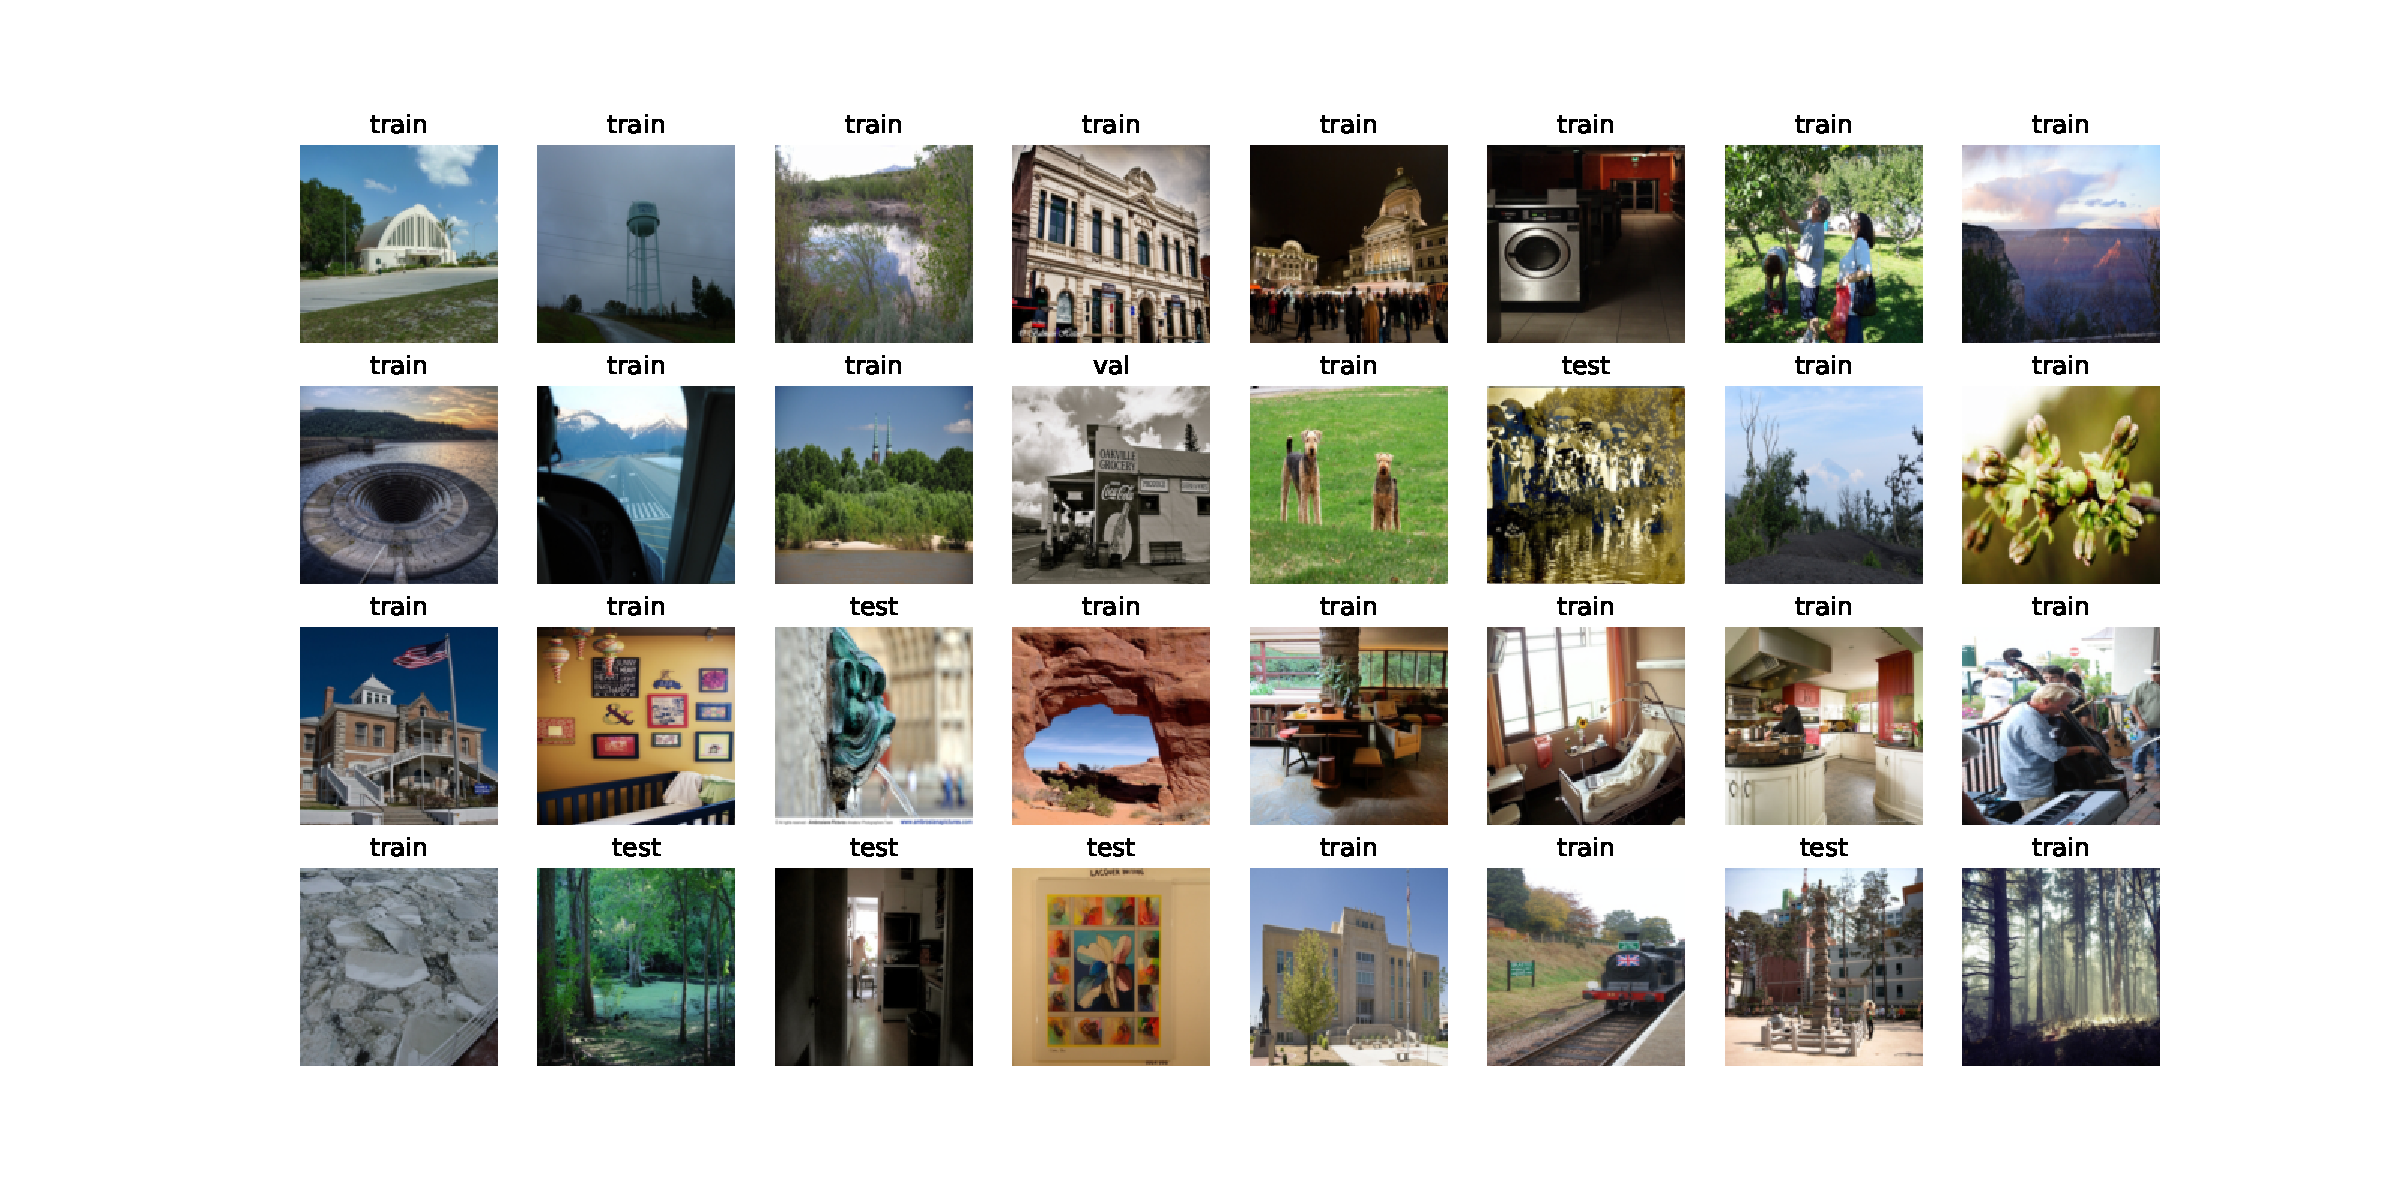
\includegraphics[width=1\textwidth]{images/places256.pdf}
    \caption{A batch of images from the Places dataset}
    \label{fig:places}
\end{figure}


\textbf{Tsinghua Dogs}

The Tsinghua Dogs dataset \cite{zouNewDatasetDog2020} is a comprehensive fine-grained classification dataset specifically designed for dog breeds. It contains a substantial collection of images, with over 65\% of them collected from real-life sources. Each breed is represented by a minimum of 200 images and a maximum of 7,449 images. According to the authors, these values are somewhat proportionate to their relative population in China. This approach ensures increased diversity for each breed compared to existing datasets. The Tsinghua Dogs dataset also provides annotated bounding boxes for each dog's whole body and head in the images, for object detection tasks, but this information is not used for this project. With a wide range of breeds included, such as Great Danes and Norwich Terriers, the dataset exhibits significant variations in appearance. While some breeds are quite similar to each other, others are rather different, which further adds to the complexity of the image classification task. 
The dataset and complete class information can be found \href{https://cg.cs.tsinghua.edu.cn/ThuDogs/}{here}.

A sample of the images from the dataset is shown in Figure ~\ref{fig:tsing}.

\begin{figure}[!htb]
    \centering
    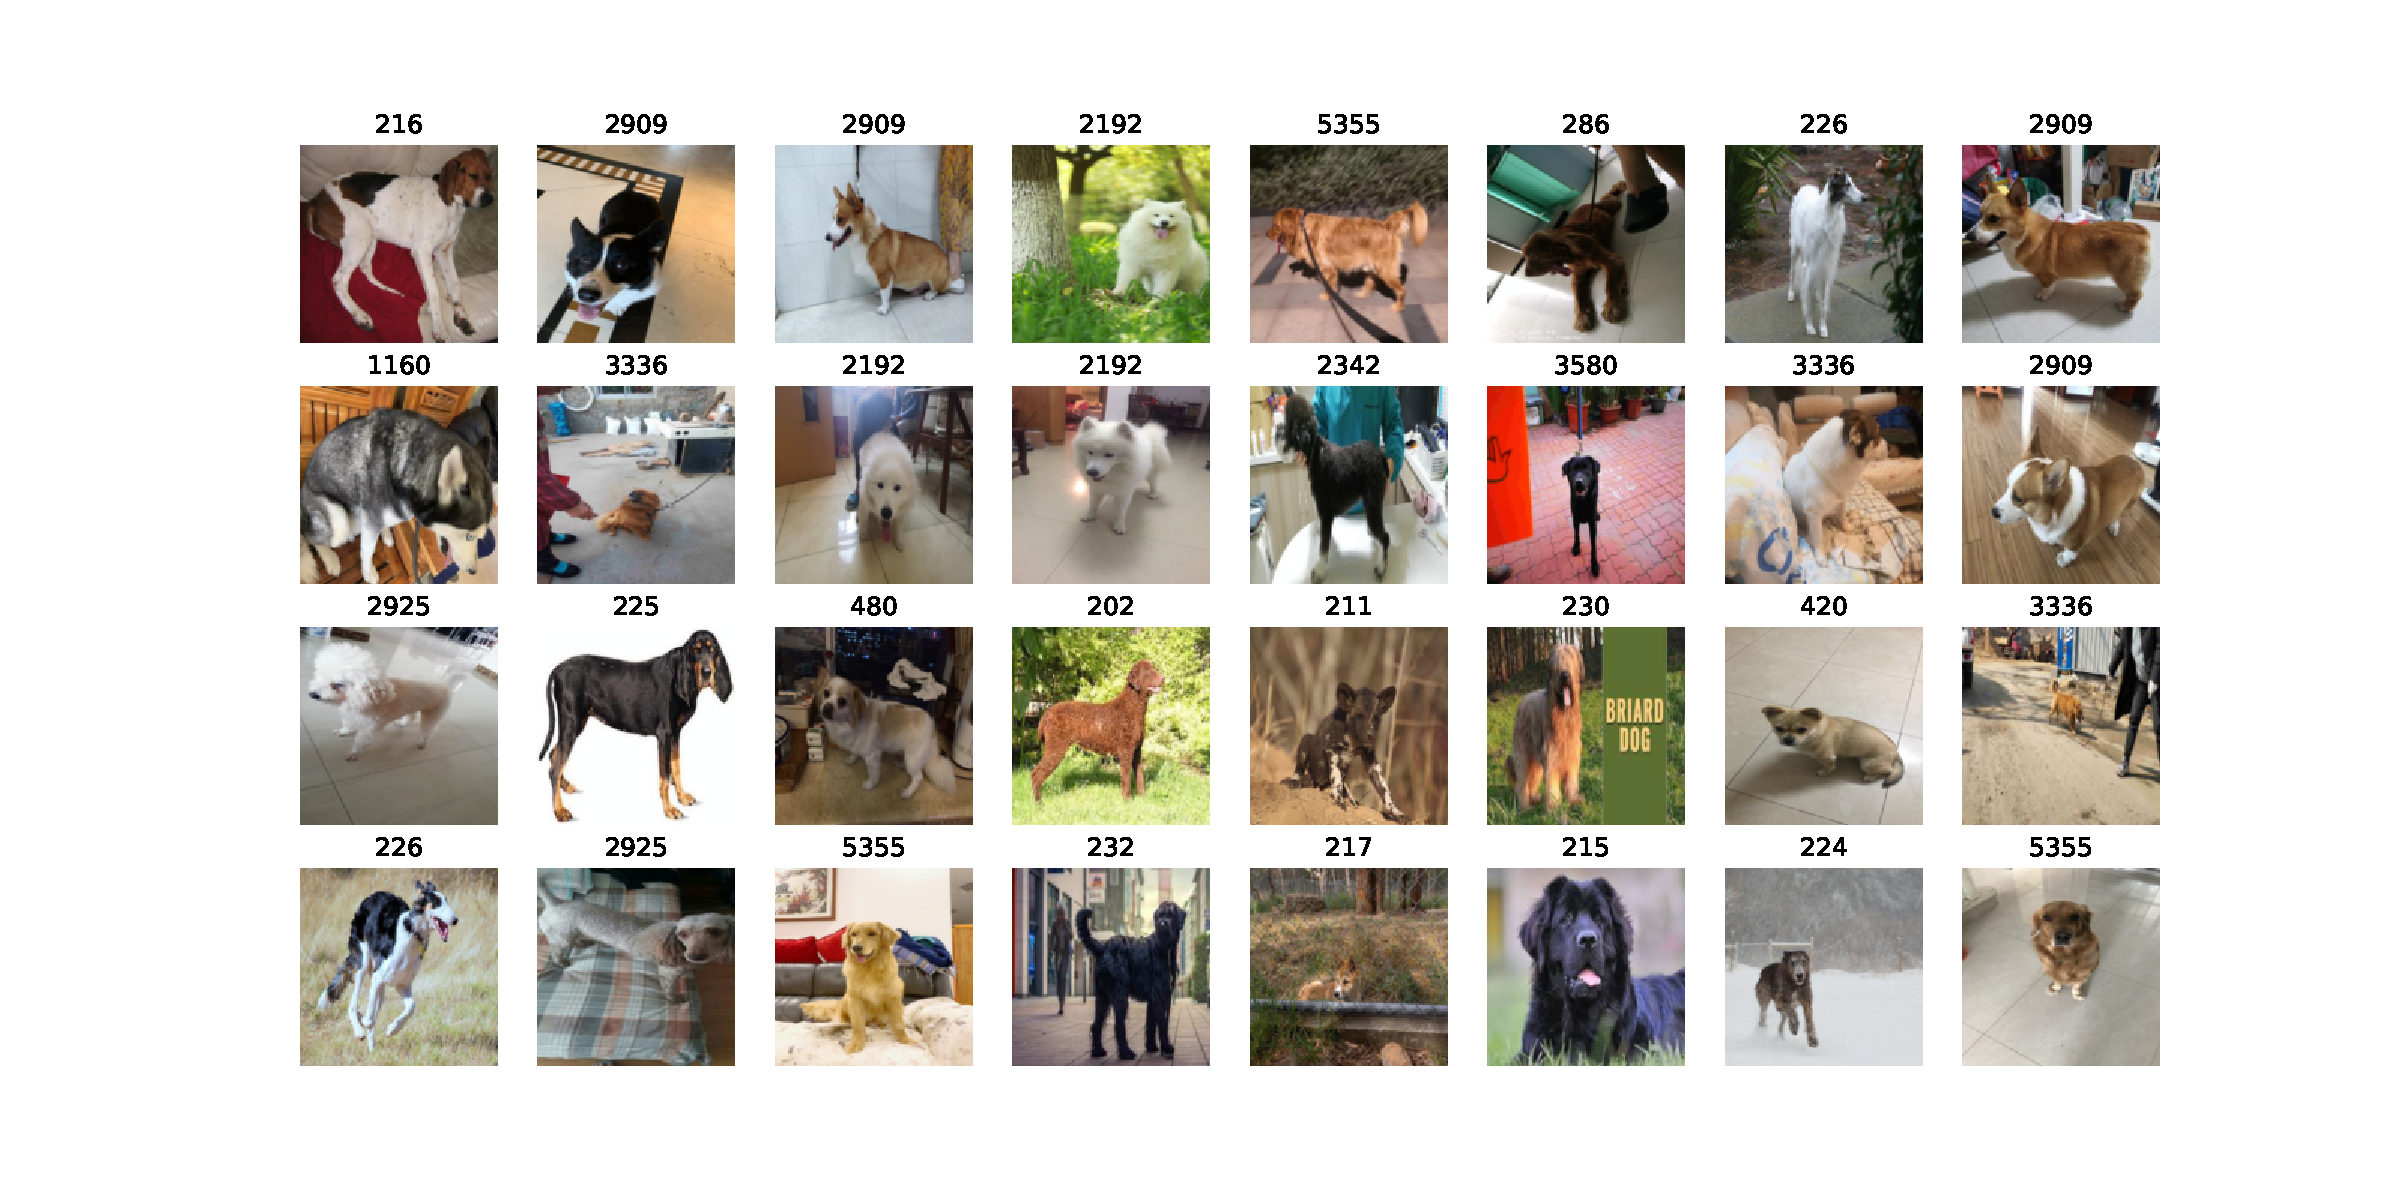
\includegraphics[width=1\textwidth]{images/tsing.pdf}
    \caption{A batch of images from the Tsinghua Dogs dataset}
    \label{fig:tsing}
\end{figure}


\subsection{Data Loading and Pre-Processing}
Since many datasets were used in the project, it was important to ensure that the data was consistent across all the experiments.  Efficient use of memory and network performance were the main priorities while designing the data loading and pre-processing steps. This section details all the tweaks, custom loaders, and pre-processing steps that were used to ensure the same.

\textbf{Data Directory structure}

The data was stored in a specific directory structure similar to the ImageNet \cite{dengImageNetLargeScaleHierarchical2009} dataset to maintain consistency across the different experiments. Every dataset is divided into training and validation folders. Most of the datasets used in the project come with this split, but a validation split is created manually for those that do not. (Note that the test split is created from the training split while training the model and is not hardcoded.) For every class in the dataset, a subfolder within the parent folder is created with the name of the class.
All the datasets used are stored in the same folder on an SSD for ease of access and performance. The directory structure is shown in Figure ~\ref{fig:dataset_structure}.
\begin{figure}[!htb]
    \centering
    \begin{forest}
        for tree={
        font=\ttfamily,
        grow'=0,
        child anchor=west,
        parent anchor=south west,
        anchor=west,
        calign=first,
        edge path={
                \noexpand\path [draw, \forestoption{edge}] (!u.south west) +(7.5pt,0) |- (.child anchor)\forestoption{edge label};
            },
        before typesetting nodes={
                if n=1
                    {insert before={[,phantom]}}
                    {}
            },
        fit=band,
        before computing xy={l=15pt},
        }
        [Dataset
            [training
                    [image001]
                    [image002]
                    [\dots]
            ]
            [validation
                    [image001]
                    [image002]
                    [\dots]
            ]
        ]
    \end{forest}
    \caption{The structure of the Dataset Directory}
    \label{fig:dataset_structure}

\end{figure}

\textbf{Custom Data Loading}

A custom data loading logic was implementd for this project. The steps are as follows:
\begin{enumerate}
    \item First, the previously generated proxy images (if they exist) are cleared from the data folder. This is done to ensure that the proxy images are not loaded by mistake.
    \item For all the remaining images, the file paths are listed and shuffled.
    \item If the current step is a Proxy step, then for every proxy image loaded, the corresponding original image is not given to the data loader. This is done so that the number of images that the networks trained with and without Proxy Attention are equal.
    \item If the \lstinline[language=Python]{subset} parameter is set to a positive value, then only a subset of the data is obtained. If not, the entire dataset is used.
    \item Using these file paths, a Pandas DataFrame is created with the file path and label. The label is generated using a label function (Ref ~\ref{sec:label_function}) based on the file path.
    \item The labels are encoded and transformed into numerical values using the \lstinline[language=Python]{LabelEncoder} and \lstinline[language=Python]{LabelBinarizer} classes from the \lstinline[language=Python]{sklearn} library. A label map and reverse label map are created and stored in memory, a step that is useful for inference.
    \item To ensure an equal percentage of samples per class (some datasets used have unequal distributions), a Stratified K-Fold oversampling is applied.
    \item Before loading the images, an additional check is performed to ensure that the images have 3 channels. If they do not, then they are converted to RGB. This check is performed as some images in the datasets could be transparent, have 4 channels, or accidentally be grayscale. Not handling these images lead to errors while training and hence they are preemptively converted to RGB.
\end{enumerate}

\textbf{Label function} \label{sec:label_function}

To ensure easy compatibility with new datasets, label functions are used to obtain labels given a file path instead of hardcoding them. This enables a uniform API that can be extended to any dataset by writing a simple lambda function.\\
In the previous step, a Pandas DataFrame with the file paths of all the images was created. To generate labels, the label function is mapped across the entire column of file paths. This function is also used to create the label map and reverse label map, that is useful for inference.\\
For example, consider the ASL dataset. The file path for a single training image is of the form \begin{verbatim}
    /media/subhaditya/datasets/ASL/asl_alphabet_train/asl_alphabet_train/A/A1.jpg
\end{verbatim} To obtain the label, a lambda function
\lstinline[language=Python]{lambda x: x.split("/")[-2]}
is used.
The label function splits the string into a list by the Unix path label separator "/" and returns the second last element in the list. Thus, the label for this image becomes \textbf{A}.\\


\textbf{Clearing proxy images} \label{sec:clearing_proxy_images}

The images are saved locally for every iteration of the Proxy Attention step. That being the case, using these generated images over further iterations of the Proxy Attention step is possible. Since these images replace the original image from the data set, it is possible to use them as a direct substitute for the original images in the data set.  Note that doing so would give the network more images when using Proxy Attention during training, which is potentially an unfair comparison. Only a single image is chosen during the data loading process to avoid this issue. Thus, this becomes a hyperparameter where the options are either to store the last generated proxy images across iterations and use those images as direct replacements for the original images or not perform the step.\\\\
In the long run, the option to persist the images across iterations could lead to the network learning artefacts introduced in prior iterations. To make sure that the networks that train with Proxy Attention are fairly compared with the ones that do not, the data loader is only passed either the original image or its substitute but not both.

\textbf{Augmentations}

Augmentations are a useful step in training neural networks and increasing robustness to new data. Since this project is a test of Proxy Attention and not of improving performance of specific architectures, a minimal set of augmentations are used. All the transforms are applied using \textbf{torchvision}.\\
For both training and validation, the images are normalized using the ImageNet statistics. This is done to maintain a standard, and also since the pretrained models used have been trained on ImageNet \cite{dengImageNetLargeScaleHierarchical2009}. The mean and standard deviation used are \begin{verbatim}
    mean = [0.485, 0.456, 0.406]
    std = [0.229, 0.224, 0.225]
\end{verbatim}
For training, the images are resized to $224\times224$. Random horizontal flips are also applied with a probability of $0.5$ along with random rotations with a maximum angle of 10 degrees and a similar probability. The images are then converted to Tensors.\\
For validation, the images are resized to $224\times224$ and then converted to Tensors. No further augmentations are applied.\\

\subsection{Architectures}
This section discusses the architectures used and the library used to implement them.

\textbf{TIMM}

The library used to load the models is called \textbf{TIMM} \cite{wightmanRwightmanPytorchimagemodelsV02023}. It is a PyTorch library that provides a vast number of models with the option of loading pretrained versions of the same. The library also provides an easy way to customize the loading options for transfer learning, including the ability to choose the number of classes, the number of layers to freeze, Global Pooling options, etc.\\
The following models were used in this project:

\textbf{VGG16}

The VGG architecture was one of the first deep networks that proposed an increase in depth using smaller filters (eg. $3 \times 3$ convs.) Increasing the depth better enabled the network to understand local image features and showed the deep learning community that increasing depth could lead to better performance. While this did hold true to a certain extent, enabling VGG to provide a good baseline over the years, it was not until ResNet \cite{heDeepResidualLearning2016} that it was possible to use these deeper networks stably. The number after the VGG (eg. VGG 18) denotes how many layers deep the network is.

The architecture of VGG16 is shown in Figure \ref{fig:vgg16}.

\begin{figure}[!htb]
    \centering
    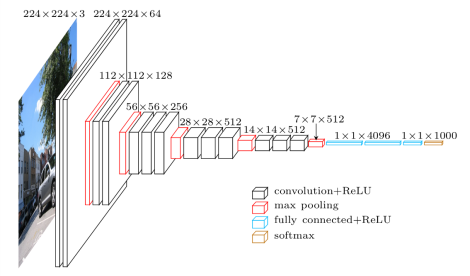
\includegraphics[width=.6\linewidth]{images/vggarch.png}
    \caption{VGG16 architecture}
    \label{fig:vgg16}
\end{figure}

\textbf{ResNet}

The ResNet architecture \cite{heDeepResidualLearning2016} introduced by He et al. changed the way deep learning models were created by stabilising the flow of gradients across the network and enabling the creation of much deeper models. He et al. addressed the problem of deeper networks failing to achieve better performance compared to their shallower counterparts by using the concept of a residual connection that enables propagating the input along with the learned features across the deeper network. The ResNet architecture directly tackled the vanishing gradient issue faced by its predecessors and paved the way for better models. The number after the ResNet (eg. ResNet 18) denotes how many layers deep the network is.

The architecture of ResNet18 is shown in Figure \ref{fig:resnet18}.
\begin{figure}[!htb]
    \centering
    \includegraphics[width=.6\linewidth]{images/resnetarch.png}
    \caption{ResNet18 architecture}
    \label{fig:resnet18}
\end{figure}

\textbf{EfficientNetB0}

EfficientNet is one of the newer architectures on this list and was proposed by Tan et al. as a means of running larger architectures with lower computational resources. The research on EfficientNet proposed a compound uniform scaling method that combined the scaling of depth, width and resolution. Using this scaling approach enables EfficientNet to scale between performance and efficiency as required. The number after the EfficientNet (eg. EfficientNet B0) denotes the scaling factor. The larger the number, the larger the number of layers and the wider the network is. This paper uses the base (B0) configuration.

The architecture of EfficientNetB0 is shown in Figure \ref{fig:efficientnetb0}.
\begin{figure}[!htb]
    \centering
    \includegraphics[width=.6\linewidth]{images/effnetarch.png}
    \caption{EfficientNetB0 architecture}
    \label{fig:efficientnetb0}
\end{figure}


\textbf{ViT Base Patch $16 \times 224$}

Transformers have been all the rage in NLP for years now, but it was not possible to use them directly in CV tasks until Dosovitskiy et al. proposed the Vision Transformer (ViT) \cite{dosovitskiyImageWorth16x162021}. The ViT considers an image as a sequence of $x \times y$ patches that enables it to use transformer architectures to images. Using a sequential representation allows capturing long-range dependences and since transformers learn "attention", using them allows the model to also learn contextual information better than regular CNNs. The ViT proved to be a landmark in CV and now approaches that use transformers dominate the SOTA in almost every niche. $x$ in this case represents the size of the patch, and in this paper a size of 16 is used. $y$ represents the size of the input image, and in this paper an image size of 224 is used. 

The architecture of ViT Base Patch $16 \times 224$ is shown in Figure \ref{fig:vit}.
\begin{figure}[!htb]
    \centering
    \includegraphics[width=.6\linewidth]{images/vitarch.png}
    \caption{ViT Base Patch $16 \times 224$ architecture}
    \label{fig:vit}
\end{figure}


\subsection{Grid Search}
A grid search was performed to test the effectiveness of Proxy Attention and to find the best combination of hyperparameters. The grid search was performed on a single machine with a single GPU. An analysis script was written to determine what trials to run instead of using a separate optimization framework (Ref ~\ref{sec:result_aggregation}).
Due to limited resources, an initial sweep over the hyperparameters was performed using a low memory network (ResNet18 \cite{heDeepResidualLearning2016}), a subset of the Stanford Dogs dataset (\cite{khoslaNovelDatasetFineGrained}), a simple gradient method (GradCAM \cite{selvarajuGradCAMVisualExplanations}) and a small number of epochs. A separate process was started for each trial in the grid search, and the memory was cleared after each trial. This process was repeated until the best combination of hyperparameters was found. Once the worst-performing parameters were eliminated, the rest of the trials were run for the other networks, datasets and methods.\\
Although it was possible to use a separate optimization framework and an algorithm like Bayesian Optimization to find the best combination of hyperparameters, the parameters were semi-automatically chosen instead due to a lack of resources and time.

\subsection{Training Resumption}
Training resumption was an important part of this project. Since Proxy Attention is applied between training runs, it was important to be able to resume training from the last checkpoint. Furthermore, since a single machine was used, resuming broken trials easily was a useful feature to have. This section discusses the challenges faced in creating this feature and the solutions implemented to overcome them.

\textbf{Checkpoints} \label{sec:checkpoints}

While checkpoints are almost always a good idea, they were especially important in this project. The Proxy Attention step is applied between training runs, and to preserve memory, it unloads the existing models and DataLoaders from the GPU. This means that when continuing training, the models and DataLoaders need to be reloaded before the next training run. Doing so would effectively reset the training process, so it was important to have checkpoints to resume training.
As part of the final analysis, the author also iterated over the trained models and compared the explainability of models trained with or without Proxy Attention. Having saved checkpoints made this process much easier.

\textbf{Broken Trials}

A challenge of training on a single machine was that the training process could be interrupted at any time. Since this project required several experiments to find the best combination of hyperparameters, it was important to be able to resume training in case of any interruptions. 

% The author initially tried using libraries such as \href{https://github.com/optuna/optuna}{Optuna} and \href{https://github.com/ray-project/ray}{Ray Tune}, but these added too much of an overhead for this project. (Ref ~\ref{sec:challenges_with_external_libraries}) A custom solution was implemented instead.\\
The objective of the solution was to be able to reload the last configuration and continue the training from there. In the implementation, the trials were generated as a list of possible configurations, and the program iterated over the list to run them. If the trial broke, the list of configurations and position of the current trial in the list was saved as a pickled dictionary. Using this saved object, the script could easily reload the last configuration and continue training without having to start from the beginning.\\
An additional useful feature of this solution was that it allowed the author to quickly patch any minor bugs without having to reiterate over the entire list of trials. This was especially useful when the author was testing the code for the first time and had to fix several bugs in the code.

\subsection{Optimizations}
The following section discusses the optimizations that were implemented to improve the performance of Proxy Attention, training the networks and reducing memory usage.

\textbf{Proxy Step specific optimizations}

The Proxy Attention step is the most computationally expensive step in the training process since it applies an XAI algorithm to each of the images in the batch of wrongly classified images. To reduce the time taken to apply the XAI algorithm, the following optimizations were implemented:
\begin{itemize}
    \item \textbf{CPU}: The CPU was used to store the wrongly classified images and labels as GPU memory is limited. The images and labels were stored during an epoch on the CPU and then passed to the GPU for the Proxy Attention step in batches.
    \item \textbf{Computational Graph}: The computational graphs of the wrongly classified images were deleted as they were not required and storing them unnecessarily increases memory usage.
    \item \textbf{Native PyTorch}: All computations were done on the GPU using PyTorch tensors, unlike many libraries that use numpy arrays. This reduced the overhead of converting between numpy arrays and PyTorch tensors and enabled the use of the GPU for all computations.
    \item \textbf{torch.where}: Replacing the pixels in the image was done using torch.where which is much faster than simply iterating over the image and replacing the pixels.
    \item \textbf{Freeing GPU memory}: The gradients were deleted from the GPU after the step was completed to reduce memory usage. This was done using \textit{del} and then calling \textit{torch.cuda.empty\_cache()} to free the memory.
    \item \textbf{Batching}: All preprocessing steps, label changes, etc., were done in batches to reduce memory usage and CPU calls.
    \item \textbf{Saving Images}: It is a known issue that saving images as \textit{png} files with no compression is slow using Pillow and thus the images were saved as \textit{jpeg} files instead. (Ref. ~\href{https://github.com/python-pillow/Pillow/issues/1211}{Github issue}). In practise, \textit{jpeg} images have smaller file sizes than \textit{png} images, which inturn reduces the additional storage required.

\end{itemize}

\textbf{Grid Search}

The major challenge with implementing a grid search was the memory usage. On a single machine, PyTorch reserves some memory for itself, and this memory is not released until the program is closed. This means that if the grid search is run sequentially, the memory usage will increase with each trial and eventually lead to a crash. The solution implemented was to run each trial as a separate process and call it from a main script. This ensured that the memory was released after each trial and the memory usage was kept in check.\\
This project did not require training multiple models simultaneously (and only a single GPU was available) and so parallelization was not required or implemented.

\textbf{Workers}

By default, PyTorch uses a single worker to load data from the SSD. This is not ideal, as the resources must be fully utilized. In this project, eight workers are to load data from the SSD, which improves the training process's performance. Note that increasing the number of workers beyond a certain point does not necessarily improve performance due to the overhead of transferring data between the CPU and GPU and might lead to detrimental effects.

\textbf{Mixed Precision}

Mixed Precision Training \cite{micikeviciusMixedPrecisionTraining2017} involves computing most of the operations in the network in half-precision (16-bit) and only using full precision (32-bit) for important operations such as the loss function. This allows for much larger batch sizes, faster training, and reduced memory usage. Micikevicius et al. also find that using Mixed Precision training does not significantly affect the model's accuracy. With all these benefits, using Mixed Precision training was a no-brainer for this project.

The only caveat is that only some operations are stable in half precision. Operations like Batch Normalization tend to break when using Mixed Precision training, and unless managed, the model fails to converge. PyTorch supports \href{https://pytorch.org/docs/stable/notes/amp_examples.html}{automatic casting} to and from half-precision and this API was used for this project.

\textbf{torch.no\_grad}

Since a single machine was used for training, it was important to reduce memory usage wherever possible. Since it was not necessary to store the gradients for the validation step as they are not used for anything, one of the ways to reduce memory consumption is to disable gradient computation for the validation step. This is done by using the \texttt{torch.no\_grad()} context manager.  The optimizer's \texttt{zero\_grad()} method is used to clear the gradients (using \texttt{set\_to\_none=True}). The additional parameter \texttt{set\_to\_none} is shown to have better performance (Refer to the ~\href{https://pytorch.org/tutorials/recipes/recipes/tuning_guide.html}{Official PyTorch tuning guide} for more information.) as it involves fewer operations.

\textbf{Pillow SIMD}

SIMD (Single Instruction, Multiple Data) is a computational technique that allows for the simultaneous execution of the same operation on multiple data points by utilizing multiple processing elements. It is particularly advantageous when compiled for specific processors, leading to improved performance in tasks such as graphics and image processing. SIMD operates synchronously and deterministically, making it suitable for operations that traditionally rely on the capabilities of a GPU. Since one of the major bottlenecks in the training process is loading images from the SSD, using SIMD operations is a way to reduce the latency. A few years ago the image processing library Pillow, used to be one of the majorly used libraries for loading images. In recent times, it has been superceded by the \href{https://github.com/uploadcare/pillow-simd}{Pillow SIMD} library, which uses SIMD instructions to improve performance. Pillow SIMD's API is a drop-in replacement for Pillow and requires no changes to the code but increases image I/O speeds by a significant margin (Refer to ~\href{https://python-pillow.org/pillow-perf/}{Benchmark comparison between Pillow and Pillow SIMD} for the official comparison).

\subsection{Tensorboard}
Tensorboard is a utility for managing and visualizing training logs. In this project, it is used to store the training configurations, metrics, images and other information that is generated during training. Since Tensorboard uses a custom file format to store this information, it can be used to store any information. Unlike many other logging utilities, Tensorboard stores all its logs locally. While storing them online might be useful in some cases, it is more difficult to manage and quite unnecessary for this project.
Another useful feature of Tensorboard is the ability to see live updates while training is in progress. This is useful for debugging and ensuring the training is progressing as expected.

\subsection{Optimizer}
While ADAM \cite{kingmaAdamMethodStochastic2014} is one of the most used optimizers in the deep learning community, Lonschiolov et al. \cite{loshchilovDecoupledWeightDecay2019} show that many libraries implement weight decay incorrectly. This finding was inspired by the choice of many researchers to use SGD with momentum instead of ADAM as it somehow seemed to perform better in many cases, but the reason for the difference in performance was not well understood. After finding the issue, Lonschiolov et al. proposed a simple fix to the weight decay implementation in ADAM, which they called ADAMW.

The error comes from the incorrect assumption that weight decay and L2 regularization are the same. While in the case of SGD, this indeed is the case, it is not true for other optimizers, especially ADAM. In the case of ADAM, weight decay first applies the update and then subtracts a portion of the weight. While L2 regularization adds the weight decay term to the gradients and then computes the moving average of the gradients and the corresponding squares before applying them to the update. Many of the deep learning libraries use L2 regularization instead of weight decay in their implementations, which leads to a significant difference in performance. Another important point to note is that the weight decay must be disabled for the optmizers as doing so will lead to L2 regularization being applied, which defeats the purpose of using ADAMW.
In this project, the ADAMW optimizer is used with a learning rate of $10^{-3}$ and a weight decay of $10^{-5}$.

\subsection{LR scheduler}
Choosing an appropriate learning rate is an important step when training a neural network. A learning rate that is too high might lead to the model overshooting the local minima when traversing the loss landscape. While a learning rate that is too low might lead to the model taking a long time to converge. A learning rate scheduler is used to find the optimal learning rate during training. The LR scheduler used in this project is the One Cycle LR scheduler proposed by Smith et al. \cite{smithSuperConvergenceVeryFast2018}.

In their paper, the authors propose a cyclic LR scheduler that moves from a lower LR to a higher LR in cycles. An LR finder is used to find the maximum LR that can be used for training. The LR finder is a simple algorithm that starts with a very low LR and increases it by a tiny amount for a number of iterations. If the loss starts to increase fast for the chosen LR, the LR finder terminates and the maximum LR is obtained. 
The One Cycle policy builds up on previous research done on warming up the learning rate at the beginning of training. While other approaches move directly to a higher LR after the initial warmup, Leslie et al. suggest a slower approach to the same. In the middle, the LR rizing can be thought of as a regularization method.

In addition to the cycle of LR, the authors also propose a cycle of momentum. They suggest that the momentum should be high at the beginning of training and should be decreased as the LR increases. This is because using a higher momentum at the beginning of training allows the model to quickly traverse the loss landscape and attempt to find local minima, but in later stages, a lower momentum is beneficial as it helps the model to converge to a local minima stably instead of overshooting it. Using a cyclic momentum removes some of the guess work involved in choosing the optimal momentum value for training, as the momentum is from lower to higher values in a cycle. 

Other benefits of the One Cycle Policy include the ability to use higher batch sizes and LRs, while also reducing the need for other regularization techniques due to the inherent regularization effect of the One Cycle Policy.

In this thesis, an LR finder is not used to find the maximum LR but set to $2\times 10^{-3}$ instead. While this is suboptimial, since the focus of this work was not to find the best performance, but just test the effects of Proxy Attention, this choice was made to reduce the number of hyperparameters that needed to be tuned. Future researchers should feel free to experiment with the LR finder to improve the accuracy further.

\subsection{Loss function}
The Cross Entropy Loss function is a popular loss function that is used in multi-class image classification tasks. Derived from the field of information theory, it uses the concept of entropy to quantifies the discrepancy between two given probability distributions. In this project, the Cross Entropy Loss is used for training the models. The formula for computing the loss is given by $\mathscr{l}(x,y) = L = \{l_{1}, ..., l_{N}\}^{T}$ where $l_{n} = -w_{y_{n}}log \frac{exp(x_{n, y_{n}})}{\Sigma_{c=1}^{C}exp(x_{n,c})}$, $x$ is the input, $y$ is the target, $C$ is the number of classes. By evaluating the predicted class probabilities against the ground truth labels, the loss function captures the dissimilarity between the predicted and actual class distributions. 

\subsection{Batch Size Finder}
To maximize training performance, a batch size finder (Ref ~\ref{fig:bsfinder} for diagram) is used to find the optimal batch size for each model.

The batch size finder algorithm is rather simple. It starts by testing for a small batch size of 2. This batch size is then successively, either incremented or decremented, based on the current GPU configuration's ability to support that batch of data.
A random batch of data with the size that is to be tested is generated and passed through the required model. If the GPU fails to accommodate the current batch of data, the loop terminates, and the required batch size is obtained. The rest of the steps required to train a network are also performed on this randomly generated data.
This algorithm remains the same for any model, data type, or other further optimizations applied (such as mixed precision training \cite{micikeviciusMixedPrecisionTraining2017}) and is robust to multiple GPUs being used for training.

\subsection{Result Aggregation} \label{sec:result_aggregation}
The biggest caveat of using Tensorboard is that the logs it generates cannot be directly queried in the interface itself. To overcome this, a custom script was written to query the logs and generate a DataFrame that combines all the logs into a single pandas DataFrame. This makes it possible to not only query the logs but also to perform any kind of analysis on them. This script can easily answer specific queries such as "What is the best accuracy across all the networks for 'gradcam++', 'dogs dataset' and 'proxy\_threshold = 0.5'?". This makes it possible to easily compare the performance of different models and .

Since the script for aggregating logs is rather useful, it was made publicly available as a \href{https://gist.github.com/SubhadityaMukherjee/58cbdf324812175233e91993b720e0bc}{Github Gist}.

\subsection{Inference}
Inference refers to using a trained model to make predictions on new data. In this project, a large number of models were trained. A separate script was created to use any of the previously trained models for inference.\\
This script follows from the result aggregation and can use queries over the dataframe generated in the previous step. Since the generated dataframe also contains the path to the saved model, this script can use that information along with the names of the architecture, dataset and other hyper-parameters to load the required models easily.
The inference script also contains functions for comparing both the accuracies and the explainability of two pre-trained models given a validation dataset or a list of images.\\
For a batch of images and given a set of hyperparameters, the script loads two models - one trained with Proxy Attention and one trained without. The same dataloader is passed through both models to obtain predictions. EigenGradCAM is used for parts of this evaluation phase to ensure a fair comparison, and since GradCAM++ was used for training, it would not be fair to use it for evaluation as well. 

\chapter{Results} \label{ch:results}
% \section{Metric Based Analysis}
% \section{Visual Based Analysis}
In line with the research questions, the evaluation section aims to quantify the performance gains obtained by using the Proxy Attention method. The section will compare the performance of networks that were trained with and without Proxy Attention based on classification metrics, and explainability improvements.

Note that complete performance logs can be found in the appendix.
\section{Accuracy}
This section explores the validation accuracy obtained by the models for different hyperparameters and datasets. Since the task at hand is a classification task, this measure is a direct comparison of the performance of the models.

\subsection{Results Per Dataset}
This subsection shows the accuracies per model for each dataset. Tabulated results can be found in the appendix.

\subsection{Tsinghua Dogs and Places256 Results}
This section shows the accuracies per model for the Tsinghua Dogs \cite{zouNewDatasetDog2020} and Places256 \cite{zhouPlaces10Million2018} datasets. The results are shown in Figure \ref{fig:tsing_places256_results}.

For the Tsinghua Dogs dataset as well as the Places256 dataset, we can see that the models trained with Proxy Attention outperform the models trained without Proxy Attention. 
ResNet50 performs the best while VGG16 performs the worst on both datasets while ResNet18 and EfficientNetB0 perform similarly. 

It is interesting to note that the performance of VGG16 trained with Proxy Attention is comparable to the performance of ResNet18 trained without Proxy Attention for both datasets. Since VGG16 performed the worst, this shows that Proxy Attention can be used to improve the performance of models regardless of how badly they initially performed.
In general, the Places256 is a much harder dataset to classify than the Tsinghua Dogs dataset and thus the accuracies are lower.

\begin{figure}[!htb]
    % \centering
    \begin{subfigure}[h]{.5\textwidth}
        \includegraphics[width=\linewidth, right]{results/tsing_results.pdf}
        \caption{Tsinghua Dogs Dataset}
    \end{subfigure}
    % \hfill
    \begin{subfigure}[h]{.5\textwidth}
        \includegraphics[width=\linewidth, left]{results/places256_results.pdf}
        \caption{Places256 Dataset}
    \end{subfigure}
    \caption{Comparing Accuracies of Models trained with and without Proxy Attention on the Tsinghua Dogs and Places256 datasets}
    \label{fig:tsing_places256_results}
\end{figure}

\subsection{Stanford Dogs and CIFAR100 Results}
This section shows the accuracies per model for the Stanford Dogs \cite{khoslaNovelDatasetFineGrained} and CIFAR100 \cite{krizhevskyLearningMultipleLayers} datasets. The results are shown in Figure \ref{fig:dogs_cifar100_results}.

Like the previous subsection, we can see that the models trained with Proxy Attention outperform the models trained without Proxy Attention. The VGG16 model here was replaced with a vision transformer model for diversity in the results. 

We see that the ViT model performs the worst on both datasets while ResNet50 performs the best. This is not to say that vision transformers are bad, but rather that in the same amount of training time, the vision transformer model was not able to learn as much as the other models. 
While the vision transformer initially performed badly, using Proxy Attention was able to improve its performance to be comparable to the performance of the other networks. This goes to show that Proxy Attention can also be used on vision transformer models to improve their performance.
\begin{figure}[!htb]
    % \centering
    \begin{subfigure}[h]{.5\textwidth}
        \includegraphics[width=\linewidth, right]{results/dogs_results.pdf}
        \caption{Stanford Dogs Dataset}
    \end{subfigure}
    % \hfill
    \begin{subfigure}[h]{.5\textwidth}
        \includegraphics[width=\linewidth, left]{results/cifar100_results.pdf}
        \caption{CIFAR100 Dataset}
    \end{subfigure}
    \caption{Comparing Accuracies of models trained with and without Proxy Attention on the Stanford Dogs and CIFAR100 datasets}
    \label{fig:dogs_cifar100_results}
\end{figure}

\subsection{Caltech101 and ASL Results}
This section shows the accuracies per model for the Caltech101 \cite{liCaltech101} and \href{https://www.kaggle.com/datasets/grassknoted/asl-alphabet}{ASL} datasets. The results are shown in Figure \ref{fig:caltech101_asl_results}.

As before, we can see that the models trained with Proxy Attention outperform those trained without Proxy Attention but the difference is not as large as the previous datasets. This could be because the Caltech101 and ASL datasets are much easier to learn than the previous datasets and thus the original models were already at a high accuracy. That being said, there was still a small improvement in accuracy for the models trained with Proxy Attention. In the odd case of the ASL dataset, the ResNet18 model trained with Proxy Attention performed worse than the model trained without Proxy Attention. Maybe this is because the ASL dataset was the easiest dataset to learn of the ones used in this thesis and thus using Proxy Attention was not necessary and hurt the performance of the model slightly.

\begin{figure}[!htb]
    % \centering
    \begin{subfigure}[h]{.5\textwidth}
        \includegraphics[width=\linewidth, right]{results/caltech101_results.pdf}
        \caption{Caltech101 Dataset}
    \end{subfigure}
    % \hfill
    \begin{subfigure}[h]{.5\textwidth}
        \includegraphics[width=\linewidth, left]{results/asl_results.pdf}
        \caption{Asl Dataset}
    \end{subfigure}
    \caption{Comparing Accuracies of models trained with and without Proxy Attention on the Caltech101 and Asl datasets}
    \label{fig:caltech101_asl_results}
\end{figure}

\subsection{Plant Disease Results}
This section shows the accuracies per model for the \href{https://www.kaggle.com/datasets/rajibdpi/plant-disease-dataset}{Plant Disease} dataset. The results are shown in Figure \ref{fig:plantdisease_results}. 

The plant disease dataset is also of a similar difficulty to the Caltech101 and ASL datasets and thus the models trained with Proxy Attention did not perform much better than the models trained without Proxy Attention. Although in most cases there was some improvement after using Proxy Attention, the ResNet50 model seemed to do better in the case where Proxy Attention was not used. 
\begin{figure}[!htb]
    \centering
    \includegraphics[width=.6\linewidth]{results/plantdisease_results.pdf}
    \caption{Comparing Accuracies of models trained with and without Proxy Attention on the Plant Disease dataset}
    \label{fig:plantdisease_results}
\end{figure}


\subsection{Results Grouped By Schedule}
This section explores the validation accuracy obtained for different step schedules. The results are shown in Figure \ref{fig:schedresnet50_results}. 
There were three types of schedules tested in this thesis: no proxy, proxy applied after half the training steps ([20, 'p',19]), and proxy applied every couple of steps ([5, 'p', 9, 'p',9, 'p',4]). The total number of training steps was 40 for all schedules with every network trained with and without Proxy Attention being given the same parameters. 

We can see that the models trained with Proxy Attention outperform the models trained without Proxy Attention for all three schedules. The schedule that performed the best was the schedule that applied Proxy Attention every couple of steps. This could be because the model was able to learn more from the Proxy Attention module when it was applied more often. While applying the proxy step in the middle of training was also able to improve the performance of the model, it can be seen that applying the proxy step multiple times was able to improve the performance even more.
\begin{figure}[!htb]
    \centering
    \includegraphics[width=.6\textwidth]{results/schedule_resnet50.pdf}
    \caption{Comparing Accuracies of models trained with and without Proxy Attention on the ResNet50 \cite{heDeepResidualLearning2016} architecture for different step schedules}.
    \label{fig:schedresnet50_results}
\end{figure}

\subsection{Results Grouped By Proxy Threshold}
This section explores the validation accuracy obtained for different Proxy thresholds. The results are shown in Figure \ref{fig:proxy_threshold}. 
The comparison was done for two different datasets: the Stanford Dogs dataset \cite{khoslaNovelDatasetFineGrained} and the Tsinghua Dogs dataset \cite{zouNewDatasetDog2020}. While the Stanford Dogs dataset is a relatively easy dataset to learn, the Tsinghua Dogs dataset is a much harder dataset to learn and thus these two datasets were chosen to see how the Proxy Threshold affects the performance of the model for datasets of different complexities. Since the comparison is done for the Proxy Threshold, different models were chosen to identify the best value across different architectures and datasets. Thus for these two figures, only comparing the value of the Proxy Threshold is important and not the actual accuracy of the model.

The results are not conclusive for this comparison and it can be said that the Proxy Threshold remains a hyperparameter that needs to be tuned for each dataset.
For the EfficientNetB0 \cite{tanEfficientnetRethinkingModel2019} trained with Proxy Attention on the Stanford Dogs dataset\cite{khoslaNovelDatasetFineGrained}, the best Proxy Threshold was 0.8, while the others had a similar performance. For the Resnet18 \cite{heDeepResidualLearning2016} trained with Proxy Attention on the Tsinghua Dogs Dataset \cite{zouNewDatasetDog2020}, the best Proxy Threshold was 0.1 and 0.85, while the others had a similar performance.
In this case, choosing a value of 0.85 for the Proxy Threshold would be a good starting point, and further tuning could be done to improve the performance of the model if needed.

\begin{figure}[!htb]
    \begin{subfigure}[h]{.5\textwidth}
        \includegraphics[width=\linewidth, right]{results/proxy_threshold_results.pdf}
        \caption{EfficientNetB0 \cite{tanEfficientnetRethinkingModel2019} trained with Proxy Attention on the Stanford Dogs dataset\cite{khoslaNovelDatasetFineGrained}}
    \end{subfigure}
    % \hfill
    \begin{subfigure}[h]{.5\textwidth}
        \includegraphics[width=\linewidth, left]{results/proxy_threshold_results_tsing.pdf}
        \caption{Resnet18 \cite{heDeepResidualLearning2016} trained with Proxy Attention on the Tsinghua Dogs Dataset \cite{zouNewDatasetDog2020}}
    \end{subfigure}
    
    \caption{Comparing Accuracies of models trained with Proxy Attention for Different Proxy Thresholds}
    \label{fig:proxy_threshold}
\end{figure}

\subsection{Results Grouped By Proxy Image Weight}
This section explores the validation accuracy obtained for different Proxy image weights. The results are shown in Figure \ref{fig:proxy_weight}. 
The comparison was done for two different datasets: the Stanford Dogs dataset \cite{khoslaNovelDatasetFineGrained} and the Tsinghua Dogs dataset \cite{zouNewDatasetDog2020}. While the Stanford Dogs dataset is a relatively easy dataset to learn, the Tsinghua Dogs dataset is a much harder dataset to learn and thus these two datasets were chosen to see how the Proxy Image Weight affects the performance of the model for datasets of different complexities. Since the comparison is done for the Proxy Image Weight, different models were chosen to identify the best value across different architectures and datasets. Thus for these two figures, only comparing the value of the Proxy Image Weight is important and not the actual accuracy of the model.

For the EfficientNetB0 \cite{tanEfficientnetRethinkingModel2019} trained with Proxy Attention on the Stanford Dogs dataset\cite{khoslaNovelDatasetFineGrained}, the best Proxy Image Weight was 0.1, while the others had a similar performance except for a weight of 0.2 which performed the worst. For the Resnet18 \cite{heDeepResidualLearning2016} trained with Proxy Attention on the Tsinghua Dogs Dataset \cite{zouNewDatasetDog2020}, the best Proxy Image Weight were 0.4 and 0.8, while the others had a similar performance.
While the results are not fully conclusive, using a Proxy Image Weight of 0.1 or 0.4 seems to be a good choice. Further, tuning is always recommended if required.

\begin{figure}[!htb]
    \begin{subfigure}[h]{.5\textwidth}
        \includegraphics[width=\linewidth, right]{results/proxy_weight_results.pdf}
        \caption{EfficientNetB0 \cite{tanEfficientnetRethinkingModel2019} trained with Proxy Attention on the Stanford Dogs dataset\cite{khoslaNovelDatasetFineGrained}}
    \end{subfigure}
    % \hfill
    \begin{subfigure}[h]{.5\textwidth}
        \includegraphics[width=\linewidth, left]{results/proxy_weight_results_tsing.pdf}
        \caption{Resnet18 \cite{heDeepResidualLearning2016} trained with Proxy Attention on the Tsinghua Dogs Dataset \cite{zouNewDatasetDog2020}}
    \end{subfigure}
    
    \caption{Comparing Accuracies of models trained with Proxy Attention for Different Proxy Image Weights}
    \label{fig:proxy_weight}
\end{figure}

\subsection{Results Grouped By Proxy Image Subset}
This section explores the validation accuracy obtained for different Proxy image subsets. The results are shown in Figure \ref{fig:proxy_subset}.
The comparison was done for two different datasets: the Stanford Dogs dataset \cite{khoslaNovelDatasetFineGrained} and the Tsinghua Dogs dataset \cite{zouNewDatasetDog2020}. While the Stanford Dogs dataset is a relatively easy dataset to learn, the Tsinghua Dogs dataset is a much harder dataset to learn and thus these two datasets were chosen to see how the Proxy Image Subset affects the performance of the model for datasets of different complexities. Since the comparison is done for the Proxy Image Subset, different models were chosen to identify the best value across different architectures and datasets. Thus for these two figures, only comparing the value of the Proxy Image Subset is important and not the actual accuracy of the model.

For the EfficientNetB0 \cite{tanEfficientnetRethinkingModel2019} trained with Proxy Attention on the Stanford Dogs dataset\cite{khoslaNovelDatasetFineGrained}, the best Proxy Image Subset was 0.2 and 0.95, while the others had a similar performance except for a subset of 0.8 which performed the worst. For the Resnet18 \cite{heDeepResidualLearning2016} trained with Proxy Attention on the Tsinghua Dogs Dataset \cite{zouNewDatasetDog2020}, the best Proxy Image Subset were 0.2 and 0.95, while 0.8 performed the worst.

Tuning the Proxy Image Subset seems to give significant improvements as compared to tuning the others, thus it is recommended to tune the Proxy Image Subset first before tuning the others. A good starting point would be to use a Proxy Image Subset of 0.2. Further, tuning is always recommended if required.
It is also interesting to note that in the case of the EfficientNetB0 \cite{tanEfficientnetRethinkingModel2019} trained with Proxy Attention on the Stanford Dogs dataset\cite{khoslaNovelDatasetFineGrained}, the model already performed quite well, and thus adding more Proxy Images did more harm than good. While in the case of the Resnet18 \cite{heDeepResidualLearning2016} trained with Proxy Attention on the Tsinghua Dogs Dataset \cite{zouNewDatasetDog2020}, the model did not perform as well, and thus adding more Proxy Images did not degrade the performance but rather improved it.

\begin{figure}[!htb]
    \begin{subfigure}[h]{.5\textwidth}
        \includegraphics[width=\linewidth, right]{results/proxy_subset_attention_results.pdf}
        \caption{EfficientNetB0 \cite{tanEfficientnetRethinkingModel2019} trained with Proxy Attention on the Stanford Dogs dataset\cite{khoslaNovelDatasetFineGrained}}
    \end{subfigure}
    % \hfill
    \begin{subfigure}[h]{.5\textwidth}
        \includegraphics[width=\linewidth, left]{results/proxy_subset_results_tsing.pdf}
        \caption{Resnet18 \cite{heDeepResidualLearning2016} trained with Proxy Attention on the Tsinghua Dogs Dataset \cite{zouNewDatasetDog2020}}
    \end{subfigure}
    
    \caption{Comparing Accuracies of models trained with Proxy Attention for different Proxy Image Subsets}
    \label{fig:proxy_subset}
\end{figure}

\section{Explanability}
This section explores the explainability of the models for different hyperparameters and datasets by using a trained model to generate attention maps for a given input image. The attention maps are compared between the same network (with the same hyperparameters) trained with and without Proxy Attention. For explanations of the results demonstrated in the section, please refer to the discussion section ~\ref{ch:discussion}.

\subsection{CIFAR 100, ResNet18, EigenGradCAM}
This section explores the explainability of the Resnet18 \cite{heDeepResidualLearning2016} trained with and without Proxy Attention on the cifar100 dataset \cite{krizhevskyLearningMultipleLayers}. The results are shown in Figure \ref{fig:resnet18_cifar100}. The attention maps were generated using EigenGradCAM \cite{banymuhammadEigenCAMVisualExplanations2021}.

Here we can see that, for most of the images, there is no difference between the predictions of the proxy attention method and the original prediction. For some of the images, such as the cockroach and the snake, the original prediction was correct, but the prediction after applying the proxy method turned out to be wrong. This does show that using proxy attention does not negatively affect the attention of the model in most cases but occasionally it does. 

\begin{figure}[!htb]
    \begin{subfigure}[b]{1\textwidth}
        \includegraphics[width=\linewidth]{images/cifar100_resnet18_noproxy_1.pdf}
        \caption{Without Proxy Attention}
    \end{subfigure}
    \begin{subfigure}[b]{1\textwidth}
        \includegraphics[width=\linewidth]{images/cifar100_resnet18_proxy_1.pdf}
        \caption{With Proxy Attention}
    \end{subfigure}
    
    \caption{Comparison of attention maps generated by resnet18 trained with and without Proxy Attention on the cifar100 dataset}
    \label{fig:resnet18_cifar100}
\end{figure}


\subsection{CIFAR 100, EfficientNetB0, EigenGradCAM}
This section explores the explainability of the EfficientNetB0 \cite{tanEfficientnetRethinkingModel2019} trained with and without Proxy Attention on the cifar100 dataset \cite{krizhevskyLearningMultipleLayers}. The results are shown in Figure \ref{fig:efficientnet_b0_cifar100}. The attention maps were generated using EigenGradCAM \cite{banymuhammadEigenCAMVisualExplanations2021}.

For this comparison, it seems that the networks predicted the results quite accurately. This also shows that using the proxy method did not negatively affect the results. For a single case of the wardrobe, the network that did not use proxy attention seemed to place higher attention on the floor while after using the proxy attention step, the model learned to focus on the wardrobe itself. It is to be noted that in the case of the roads, the model trained with proxy attention seemed to make a mistake.

\begin{figure}[!htb]
    \begin{subfigure}[b]{1\textwidth}
        \includegraphics[width=\linewidth]{images/cifar100_efficientnet_b0_noproxy_0.pdf}
        \caption{Without Proxy Attention}
    \end{subfigure}
    \begin{subfigure}[b]{1\textwidth}
        \includegraphics[width=\linewidth]{images/cifar100_efficientnet_b0_proxy_0.pdf}
        \caption{With Proxy Attention}
    \end{subfigure}

    \caption{Comparison of attention maps generated by efficientnet\_b0 trained with and without Proxy Attention on the cifar100 dataset}
    \label{fig:efficientnet_b0_cifar100}
\end{figure}
    


\subsection{CIFAR 100, ViT , EigenGradCAM}
This section explores the explainability of the ViT \cite{dosovitskiyImageWorth16x162021} trained with and without Proxy Attention on the cifar100 dataset \cite{krizhevskyLearningMultipleLayers}. The results are shown in Figure \ref{fig:vit_cifar100}. The attention maps were generated using EigenGradCAM \cite{banymuhammadEigenCAMVisualExplanations2021}.

This comparison is for the ViT. Since the transformer network learns the images in patches, and no other preprocessing step was applied, the attention map is denoted as localized points across the image and not complete attention like the CNNs before. In this case, it did seem that using proxy attention, helped the network focus quite a bit on the correct regions of the image. For example, in the lion, man, couch, beaver, et cetera. The model had initially learned the wrong part of the image, but in the case of the proxy intention model, the correct part of the image was learned. Only in the case of the cloud, does it seem that the model trained with proxy attention learned the wrong part of the image.

    \begin{figure}[!htb]
        \begin{subfigure}[b]{1\textwidth}
            \includegraphics[width=\linewidth]{images/gpp_cifar100_vit_base_patch16_224_noproxy_0.pdf}
            \caption{Without Proxy Attention}
        \end{subfigure}
        \begin{subfigure}[b]{1\textwidth}
            \includegraphics[width=\linewidth]{images/gpp_cifar100_vit_base_patch16_224_proxy_0.pdf}
            \caption{With Proxy Attention}
        \end{subfigure}
        \caption{Comparison of attention maps generated by vit\_base\_patch16\_224 trained with and without Proxy Attention on the cifar100 dataset}
        \label{fig:vit_cifar100}
    \end{figure}
    


\subsection{CIFAR 100, ViT , GradCamPlusPlus}
This section explores the explainability of the ViT \cite{dosovitskiyImageWorth16x162021} trained with and without Proxy Attention on the cifar100 dataset \cite{krizhevskyLearningMultipleLayers}. The results are shown in Figure \ref{fig:vit_cifar100}. The attention maps were generated using GradCamPlusPlus \cite{chattopadhayGradCAMGeneralizedGradientBased2018}.

The results of this comparison are similar to the one above. In the case of the possum, the man had to try the model relearnt the attention map correctly. While in the case of the train, it did seem that the model learned to associate the sky with the presence of a train track. 

\begin{figure}[!htb]
        \begin{subfigure}[b]{1\textwidth}
            \includegraphics[width=\linewidth]{images/cifar100_vit_base_patch16_224_noproxy_0.pdf}
            \caption{Without Proxy Attention}
        \end{subfigure}
        \begin{subfigure}[b]{1\textwidth}
            \includegraphics[width=\linewidth]{images/cifar100_vit_base_patch16_224_proxy_0.pdf}
            \caption{With Proxy Attention}
        \end{subfigure}
        \caption{Comparison of attention maps generated by vit\_base\_patch16\_224 trained with and without Proxy Attention on the cifar100 dataset}
        \label{fig:vit_cifar100}
    \end{figure}
    


\subsection{Tsinghua Dogs, ResNet50 , GradCamPlusPlus}
This section explores the explainability of the ResNet50 \cite{heDeepResidualLearning2016} trained with and without Proxy Attention on the Tsinghua dogs dataset \cite{zouNewDatasetDog2020}. The results are shown in Figure \ref{fig:resnet50_tsing}. The attention maps were generated using GradCamPlusPlus \cite{chattopadhayGradCAMGeneralizedGradientBased2018}.

Both the models in this case were accurate enough for the results to be similar. In the case of the second column of images, the model trained with proxy attention seemed to localize the position of the dogs better.  In a few of the other examples of the model trained with proxy attention, more focus is placed on the faces of the dogs, which would probably have helped the model recognize the breeds better.

\begin{figure}[!htb]
    \begin{subfigure}[b]{1\textwidth}
        \includegraphics[width=\linewidth]{images/gpp_tsing_resnet50_noproxy_0.pdf}
        \caption{Without Proxy Attention}
    \end{subfigure}
    \begin{subfigure}[b]{1\textwidth}
        \includegraphics[width=\linewidth]{images/gpp_tsing_resnet50_proxy_0.pdf}
        \caption{With Proxy Attention}
    \end{subfigure}
    \caption{Comparison of attention maps generated by resnet50 trained with and without Proxy Attention on the Tsinghua Dogs dataset}
    \label{fig:resnet50_tsing}
\end{figure}


\subsection{Tsinghua Dogs, ResNet18, EigenGradCAM}
This section explores the explainability of the ResNet18 \cite{heDeepResidualLearning2016} trained with and without Proxy Attention on the Tsinghua dogs dataset \cite{zouNewDatasetDog2020}. The results are shown in Figure \ref{fig:resnet18_tsing}. The attention maps were generated using EigenGradCAM \cite{banymuhammadEigenCAMVisualExplanations2021}.

The results obtained for this comparison are also similar to the ones above. In some cases, though, the model trained with proxy attention seemed to learn the wrong part of the image, even though it had initially got it correct.

\begin{figure}[!htb]
    \begin{subfigure}[b]{1\textwidth}
        \includegraphics[width=\linewidth]{images/tsing_resnet18_noproxy_0.pdf}
        \caption{Without Proxy Attention}
    \end{subfigure}
    \begin{subfigure}[b]{1\textwidth}
        \includegraphics[width=\linewidth]{images/tsing_resnet18_proxy_0.pdf}
        \caption{With Proxy Attention}
    \end{subfigure}
    \caption{Comparison of attention maps generated by resnet18 trained with and without Proxy Attention on the Tsinghua Dogs dataset}
    \label{fig:resnet18_tsing}
\end{figure}

\chapter{Discussion} \label{ch:discussion}
\section{Research Questions}

 
The section discusses our results with respect to the research questions proposed in the study.
\begin{itemize}
\item \textbf{Is it possible to create an augmentation technique that uses Attention maps :} From our experiments, we do find that it is possible to use gradient based techniques as an augmentation step to create a proxy of the attention mechanism. Using proxy attention improves performance with a minimal increase in computation. Thus we can say that this research objective was completely fulfilled.
\item \textbf{Is it possible to approximate the effects of Attention from ViTs in a CNN without changing the architecture :} While proxy attention does incorporate the results of gradient based techniques while training to help guide the networks attention better, we do see that the type of attention exhibited is not the same as that of a vision transformer. Since the latter uses patches of a fixed size to feed into the network generating an attention map is related to the size of the patch as well. In the case of CNNs, the attention map is generated per pixel in the input image. To some extent it seems to be more useful to look at the attention map generated by CNN as compared to that of a vision transformer. We do also see that the CNN takes a lot less computational resources and time to train as compared to the vision transformer while also having a slightly more useful attention map. 

This being the case, this objective can also said to be completed, but the results were slightly different from what was initially expected. Future work could tackle this discrepancy by including research from quantifying attention flows in Transformers. \cite{abnarQuantifyingAttentionFlow2020}
\item \textbf{Is it possible to make a network converge faster and consequently require less data using the outputs from XAI techniques :} From our results we do indeed see that using the outputs of gradient based techniques as part of proxy attention does have the network converge faster. As for using less data, although the need for data is not replaced, proxy attention does improves performance without the addition of new data or any modifications to the architecture. Thus we can say that this objective was also fulfilled.
\item \textbf{Does using Proxy Attention impact the explainability positively :} From comparing the attention maps, generated by networks and without proxy attention, we can see that the former does have better explanations. In most cases, using proxy attention does help guide the network to the important parts of the image. It is to be noted that in some cases using our method does make the network focus on the wrong part of the image, but this happens in frequently, and is not an inherent flaw of the method.

Although this does not impact the final performance, some possible reasons of this happening are discussed below. That being the case, we can also say that this objective was mostly fulfilled, except for the occasional mistake.
\end{itemize}


\section{Discussion of Results}
The following observations were made based on the results of both the explainability, and the accuracy obtained for different models trained with and without proxy attention on a multitude of datasets.
\begin{itemize}
 \item In general, using proxy attention to training model improves performance, regardless of the dataset and model used.
 \item Applying the proxy attention step multiple times in the training process does seem to improve performance, depending on how many times it was applied. But the rate of change of performance is not linear, and of course applying the proxy step multiple times does increase amount of compute required.
 \item The proxy attention step also seems to improve the results of the vision transformer and helps it learn to focus on the right regions of the image faster.
 \item From the results, we can see that it is not always beneficial to apply the proxy attention step to every image that the model predicted wrong. One of the hyper parameters was the subset of images that were passed to proxy attention. It was observed that if a network already has learnt a good representation of the data, giving it too many images might negatively affect performance. But if optimal performance has not been reached yet, then varying the Proxy Image subset parameter seems to be beneficial.
 \item Tuning Proxy Weight and Proxy Threshold is not really necessary but can help slightly improve performance. Using the values we suggested is enough in most cases.
 \item For easier datasets, using Proxy Attention sometimes degrades the performance and explainability of the network. For harder tasks and networks that do not initially learn well though, applying the method boosts accuracy.
 \item In most cases results indicate that models trained with Proxy Attention have improved explainability, for both CNNs and the Vision Transformer.
\end{itemize}



\section{Limitations of Proxy Attention}
\begin{itemize}
\item \textbf{Hyperparameters :} The research in this paper discusses quite a few hyper parameters. While optimal values of most of the hyper parameters have been found and discussed, some of them such as the Proxy Weight and Proxy Threshold seem to have more subtle effects. Although some recommended values for these parameters have been discussed, they seem to be reliant on the dataset used as well. That being the case, it would be required to further test these hyper parameters to improve performance on a case to case basis. This further testing is a very common part of most deep learning algorithms, but since Proxy Attention was created with the intent of reducing the computational cost of training a neural network, these additional tests do not support the objective fully. 

But on the other hand, we noticed that it was possible to get an improvement in performance even with the values we suggested for these hyperparameters. This means that having to do these additional tests is an optional part of the algorithm, and depending on the use case and the amount of performance tuning required, it is possible to use them to further improve performance if necessary.
\item \textbf{Attention :} One of the motives of Proxy Attention was to be able to imitate the effects of the attention mechanism to further improve performance by guiding a CNN based on its mistakes. From our results, we do indeed see that using our method does improve the attention of the network and helps it to better figure out the important parts of the image. But, in some cases using Proxy Attention does influence the network negatively. Although this is not extremely common, and for the most part does not really impact performance all that much it is worth noting that further research is needed in this particular case. 

One of the possible reasons that this happens is because the network does learn different representations at different parts of the training process. In the case where the network initially gets the attention map correct and then later gets it wrong, it might be because at that particular time step, the network has not fully developed a representation for that class yet. To support the statement, it is valuable to see that even though at the time steps considered, some of the attention map seem to be wrong, in the long run the performance of the network does not seem to be affected. For almost all our tests, we did see an increase in performance when using Proxy Attention.
\item \textbf{Better Scheduling :} Unlike data augmentation, the Proxy Attention step is not applied for every epoch. Since our method relies on the understanding of the network itself, applying it for every epoch seems counterintuitive. It does take any network time to learn, and if the step was applied for every epoch, it might actually end up destabilising training. That being the case, we did test multiple schedules with varying intervals of applying Proxy Attention. From our experiment, we did see that applying our method multiple times does seem to improve performance but there does not seem to be a linear increase in performance with increasing number of applications of Proxy Attention. 

In the initial stages of training neural networks, the network of course has not had time to learn better representation. While in the later stages of training, the network does have a better understanding of the data distribution and in turn can be used to generate better attention maps. That being the case, having a more semi automatic schedule would be beneficial. This schedule was not tested in this research, but future work could look at implementing a scheduler based on the performance of the network across training. An algorithm similar to that of a learning rate scheduler could be used.
\end{itemize}

\section{Future Work}
While the results of this thesis are promising, there is still a lot of room for improvement. The following are some of the possible future directions for this work:
\begin{itemize}
    \item \textbf{Schedules:} Currently, the number of Proxy Steps and the number of images used for the Proxy Step are fixed. It would be interesting to schedule both of these based on the validation performance. For example, if the validation performance is not improving, we can increase the number of Proxy Steps and the number of images used for the Proxy Step.
    \item \textbf{More XAI methods:} We have only used a tiny subset of XAI methods for this thesis. It would be interesting to experiment with more XAI methods (eg: other methods from the literature survey) and see if they can be used to improve the performance of Proxy Attention.
    \item \textbf{Smoothing Attention Maps:} The attention maps generated by the XAI methods are noisy. While no extra smoothing was used in this thesis, it would be useful to experiment with smoothing the attention maps before using them for the Proxy step. An example of a potentially suitable smoothing method is Eigen Smoothing \cite{jacobPyTorchLibraryCAM2021}.
    \item \textbf{Better Attention Maps for ViT:} This research used the base vision transformer model but Abnar et al. \cite{abnarQuantifyingAttentionFlow2020} in their paper, find that the attention maps generated by a vision transformer are pretty unreliable due to self attention, combining different representations across layers of the transformer. While using self attention does lead to massive improvements and performance for Transformers, using these attention weights is an unreliable method of generating proper explanations. Thus future work could take their work into account to have a better comparison between CNNs and Transformers.
\end{itemize}

\section{General Discussion} 
\subsection{Data Augmentation}
\begin{itemize}
    \item \textbf{Why not provide annotations and object position: }Datasets that contain annotations and positions are not easy to compile. For custom tasks, it is quite difficult to obtain such datasets. That being the case, Proxy Attention is a good alternative as it does not require any extra information.

    \item \textbf{Why not apply it every epoch like augmentation: } Applying Proxy Attention every epoch comes with certain caveats. Since gradient maps are being computed for multiple images, this process is slightly more computationally expensive than standard training. Doing so might also lead to overfitting as the network is given too much feedback. Since Proxy Attention relies on the model's predictions, giving the network time to learn is a good idea.

    \item \textbf{Isn't it the same as giving more images to the model: } This is somewhat true. Proxy Attention provides similar benefits to augmentation but with more specific information. In the models tested, an equal number of images were given to each model. Models trained with Proxy Attention and those trained without it received the same number of images. For example, if the modified image was present, the original image was not passed to the network to maintain fairness.
\end{itemize}

\subsection{Other Domains}
\begin{itemize}
\item \textbf{Why is it not SSL:} SSL involves using generating pseudo-labels in the case of real labels not being available and Proxy Attention simply uses Gradient based methods to guide the network to the correct parts of the image. Future research could also explore using Proxy Attention together with SSL.
\item \textbf{Why not use distillation:} Proxy Attention was created with the hope of speeding up training with minimal increase in the usage of computational resources. Distillation refers to using a model that was already trained on a similar task to improve the learning process of the current model. While distillation works very well and is useful in many regards, it goes against the aims of Proxy Attention as training the original network would have used up even more computational resources. That is not to say that distillation is not advantageous, but just that it is just not in the scope of this study.
\end{itemize}

\subsection{Model Architecture and Attention Modules}
\begin{itemize}
    \item \textbf{Why not just use a Transformer: }The use of Transformers was indeed tested, but they are more computationally expensive and not as easy to train as Convolutional Neural Networks (CNNs). The objective of the study was to explore whether the effects of the attention module could be approximated using gradient-based techniques. As a side note though, Proxy Attention, which also works with Transformers and also seems to improve the results of the model.
    \item \textbf{Why not modify the network architecture to include attention modules: }Proxy Attention was developed as a general technique that can be applied to any network architecture, not limited to CNNs. Many of the surveyed papers required specialized architectures, which can be counterintuitive and not always feasible to implement. Thus, Proxy Attention offers a more versatile approach for improving performance by only modifying the training process.
\end{itemize}

\subsection{Gradient Based Techniques}
\begin{itemize}
    \item \textbf{Why use a different gradient-based technique for the results: } To ensure fairness in the evaluation process, it is important to use a different gradient-based technique for the results. Neural networks excel at approximating transformations, so if the same technique is used for both training and evaluation, the network may end up learning to approximate the technique itself instead of learning where to look, which would defeat the whole point of Proxy Attention. Testing with a different technique ensures a fair comparison and avoids bias in the evaluation.

    % \item \textbf{Combining gradient-based techniques with training is a bad idea, right: } This study was conducted specifically to investigate the feasibility of combining gradient-based techniques with training. While further rigorous testing is necessary to gain a deeper understanding of why and to what extent this approach works, our findings indicate that it is a promising starting point. Combining gradient-based techniques with training can lead to improved performance, but more research is needed to fully comprehend the underlying mechanisms and limitations of this approach.
\end{itemize}

\subsection{Hyperparameters}
\begin{itemize}
    \item \textbf{Why so many hyperparameters: } Since Proxy Attention is a novel technique, it necessitated testing multiple hyperparameters to determine which ones yield the best results. The extensive exploration of hyperparameters enabled the author to narrow down the search space for future experiments and focus only on the most effective ones. Varying the hyperparameters also allowed the author to examine the impact of different components of the pipeline, leading to a better understanding of the overall effects of using Proxy Attention.

    \item \textbf{Why do some of the hyperparameters not seem to be very sensitive: } In certain datasets, the hyperparameters may not exhibit significant effects. This could be attributed to the network already performing well enough on those datasets, rendering the hyperparameter variations less impactful. While there are theoretical expectations of certain effects, such as faster convergence, the practical results may not always demonstrate a substantial improvement in our studies. But although the effects may not be pronounced, they still contribute to enhancing the overall results to a certain degree. If nothing else, they do not seem to have a negative impact on the results, so they are still worth exploring.
\end{itemize}

\subsection{Stability and Training Effects}
\begin{itemize}
    \item \textbf{Will this destabilize training: } Some predictions that were previously classified correctly may become incorrect when using Proxy Attention. It is also to be noted that this does not seem to occur too frequently, so it is not a major concern. While this phenomenon does not appear to destabilize the training process, it does make the network more sensitive to applying Proxy Attention too frequently. The results indicate that applying Proxy Attention improves performance regardless, but it is not recommended to apply it every epoch. 

    \item \textbf{In later iterations, what happens if a correctly predicted image is wrongly classified: } Since the images generated through Proxy Attention are not persistent, the network should be capable of recovering from such misclassifications. In the worst-case scenario, the network will be trained on a slightly modified image, which is not necessarily detrimental. Moreover, the network has previously encountered the original image, so it should be able to learn a better representation of the image through subsequent iterations.

\end{itemize}

\subsection{Challenges with External Libraries} \label{sec:challenges_with_external_libraries}
Some of the challenges that were faced while using external libraries are as follows:
\begin{enumerate}
    \item \textbf{GPU cache}: While Ray Tune and Optuna manage resources efficiently, they did not clear the GPU cache effectively. PyTorch, by default, holds on to the GPU cache and does not release it until the program is closed for efficiency. This would not be a problem for a single training run, but if many trials were being run, the cache would quickly fill up and cause the training to crash. This does not imply that using Proxy Attention makes it impossible to use such libraries but that it was easier to implement a custom solution.
    \item \textbf{Cluster} : Both libraries were written to enable running large-scale experiments over multiple machines. While this would be useful for a large-scale project, it added unnecessary complexity to this project as all the experiments were run on a single machine.
    \item \textbf{Grid Search} : Both libraries mentioned above were designed for hyperparameter tuning and to implement multiple grid search variants. While this would be useful, it would stop many trials that would eventually be useful to analyze. In this project, it was important to have results for each of the trials, and since the author could not find a way to disable the default Early Stopping behaviour as part of the grid search, a simple trial generation algorithm was created instead.
\end{enumerate}

\chapter{Conclusion} \label{ch:conclusion}

\section{Lessons Learned}
The lessons learned from this thesis are as follows:
\begin{itemize}
    \item \textbf{Combining research from different domains to create a novel method: } This thesis taught me how to combine research from different domains to create a novel method. In this case, we combined research from the domains of XAI and Augmentation to create a novel augmentation technique.
    \item \textbf{Hyperparameter Tuning: } We performed a large number of experiments with different hyperparameters and models to test the robustness of the method and find the best configuration. Doing so taught me the importance of hyperparameter tuning.
    \item \textbf{Memory Leaks: }We encountered a lot of memory leaks while working on the code for this thesis, and in the process learned how to debug and fix them. 
    \item \textbf{Functional code vs OOP: }We wrote the code for this thesis in a functional style instead of an object oriented style as a personal experiment. This made it easy to reuse certain parts of the code and modify others. Doing so taught me the importance of writing functional code.
    \item \textbf{Augmentation: }We learned a lot about augmentation while working on this thesis. We learned about the different types of augmentations, how to implement them, and how to use them to improve the performance of CNNs.
    \item \textbf{XAI: }We also learned a lot about XAI while working on this thesis. 
    \item \textbf{Training Loop: } Previous to this thesis, the author had only used the training loop provided by higher level libraries. However, for this thesis, we had to implement the training loop from scratch. Doing so taught the author a lot about the different components of the training loop and how to configure them for optimal performance and modify them to suit the needs of the project.
\end{itemize}




\chapter{Appendix} \label{ch:appendix}
\section{Intuition Figure}
\section{Batch Finder Algorithm}
This section shows pipeline used to find the optimal batch size for training. 
\begin{figure}[!htb]
    \centering
    \includegraphics[width=0.6\linewidth]{images/batchsizefinder.pdf}
    \caption{Diagramatic representation of the Batch Size Finder Algorithm}
    \label{fig:bsfinder}
\end{figure}

\section{Additional Explanability Results}
This section contains additional results for the explainability experiments. 

\begin{figure}[!htb]
    \centering
    \begin{subfigure}[b]{1\textwidth}
        \includegraphics[width=\textwidth]{images/cifar100_resnet18_noproxy_1.pdf}
        \caption{Without Proxy Attention}
    \end{subfigure}
    \hfill
    \begin{subfigure}[b]{1\textwidth}
        \includegraphics[width=\textwidth]{images/cifar100_resnet18_proxy_1.pdf}
        \caption{With Proxy Attention}
    \end{subfigure}
    \caption{Comparison of attention maps generated by resnet18 trained with and without Proxy Attention on the cifar100 dataset using EigenGradCAM}
\end{figure}


\begin{figure}[!htb]
    \centering
    \begin{subfigure}[b]{1\textwidth}
        \includegraphics[width=\textwidth]{images/cifar100_resnet18_noproxy_2.pdf}
        \caption{Without Proxy Attention}
    \end{subfigure}
    \hfill
    \begin{subfigure}[b]{1\textwidth}
        \includegraphics[width=\textwidth]{images/cifar100_resnet18_proxy_2.pdf}
        \caption{With Proxy Attention}
    \end{subfigure}
    \caption{Comparison of attention maps generated by resnet18 trained with and without Proxy Attention on the cifar100 dataset using EigenGradCAM}
\end{figure}


\begin{figure}[!htb]
    \centering
    \begin{subfigure}[b]{1\textwidth}
        \includegraphics[width=\textwidth]{images/cifar100_resnet18_noproxy_3.pdf}
        \caption{Without Proxy Attention}
    \end{subfigure}
    \hfill
    \begin{subfigure}[b]{1\textwidth}
        \includegraphics[width=\textwidth]{images/cifar100_resnet18_proxy_3.pdf}
        \caption{With Proxy Attention}
    \end{subfigure}
    \caption{Comparison of attention maps generated by resnet18 trained with and without Proxy Attention on the cifar100 dataset using EigenGradCAM}
\end{figure}




\begin{figure}[!htb]
    \centering
    \begin{subfigure}[b]{1\textwidth}
        \includegraphics[width=\textwidth]{images/cifar100_efficientnet_b0_noproxy_1.pdf}
        \caption{Without Proxy Attention}
    \end{subfigure}
    \hfill
    \begin{subfigure}[b]{1\textwidth}
        \includegraphics[width=\textwidth]{images/cifar100_efficientnet_b0_proxy_1.pdf}
        \caption{With Proxy Attention}
    \end{subfigure}
    \caption{Comparison of attention maps generated by efficientnet\_b0 trained with and without Proxy Attention on the cifar100 dataset using EigenGradCAM}
\end{figure}


\begin{figure}[!htb]
    \centering
    \begin{subfigure}[b]{1\textwidth}
        \includegraphics[width=\textwidth]{images/cifar100_efficientnet_b0_noproxy_2.pdf}
        \caption{Without Proxy Attention}
    \end{subfigure}
    \hfill
    \begin{subfigure}[b]{1\textwidth}
        \includegraphics[width=\textwidth]{images/cifar100_efficientnet_b0_proxy_2.pdf}
        \caption{With Proxy Attention}
    \end{subfigure}
    \caption{Comparison of attention maps generated by efficientnet\_b0 trained with and without Proxy Attention on the cifar100 dataset using EigenGradCAM}
\end{figure}


\begin{figure}[!htb]
    \centering
    \begin{subfigure}[b]{1\textwidth}
        \includegraphics[width=\textwidth]{images/cifar100_efficientnet_b0_noproxy_3.pdf}
        \caption{Without Proxy Attention}
    \end{subfigure}
    \hfill
    \begin{subfigure}[b]{1\textwidth}
        \includegraphics[width=\textwidth]{images/cifar100_efficientnet_b0_proxy_3.pdf}
        \caption{With Proxy Attention}
    \end{subfigure}
    \caption{Comparison of attention maps generated by efficientnet\_b0 trained with and without Proxy Attention on the cifar100 dataset using EigenGradCAM}
\end{figure}




\begin{figure}[!htb]
    \centering
    \begin{subfigure}[b]{1\textwidth}
        \includegraphics[width=\textwidth]{images/gpp_cifar100_vit_base_patch16_224_noproxy_1.pdf}
        \caption{Without Proxy Attention}
    \end{subfigure}
    \hfill
    \begin{subfigure}[b]{1\textwidth}
        \includegraphics[width=\textwidth]{images/gpp_cifar100_vit_base_patch16_224_proxy_1.pdf}
        \caption{With Proxy Attention}
    \end{subfigure}
    \caption{Comparison of attention maps generated by vit\_base\_patch16\_224 trained with and without Proxy Attention on the cifar100 dataset using EigenGradCAM}
\end{figure}


\begin{figure}[!htb]
    \centering
    \begin{subfigure}[b]{1\textwidth}
        \includegraphics[width=\textwidth]{images/gpp_cifar100_vit_base_patch16_224_noproxy_2.pdf}
        \caption{Without Proxy Attention}
    \end{subfigure}
    \hfill
    \begin{subfigure}[b]{1\textwidth}
        \includegraphics[width=\textwidth]{images/gpp_cifar100_vit_base_patch16_224_proxy_2.pdf}
        \caption{With Proxy Attention}
    \end{subfigure}
    \caption{Comparison of attention maps generated by vit\_base\_patch16\_224 trained with and without Proxy Attention on the cifar100 dataset using EigenGradCAM}
\end{figure}


\begin{figure}[!htb]
    \centering
    \begin{subfigure}[b]{1\textwidth}
        \includegraphics[width=\textwidth]{images/gpp_cifar100_vit_base_patch16_224_noproxy_3.pdf}
        \caption{Without Proxy Attention}
    \end{subfigure}
    \hfill
    \begin{subfigure}[b]{1\textwidth}
        \includegraphics[width=\textwidth]{images/gpp_cifar100_vit_base_patch16_224_proxy_3.pdf}
        \caption{With Proxy Attention}
    \end{subfigure}
    \caption{Comparison of attention maps generated by vit\_base\_patch16\_224 trained with and without Proxy Attention on the cifar100 dataset using EigenGradCAM}
\end{figure}



\begin{figure}[!htb]
    \centering
    \begin{subfigure}[b]{1\textwidth}
        \includegraphics[width=\textwidth]{images/cifar100_vit_base_patch16_224_noproxy_1.pdf}
        \caption{Without Proxy Attention}
    \end{subfigure}
    \hfill
    \begin{subfigure}[b]{1\textwidth}
        \includegraphics[width=\textwidth]{images/cifar100_vit_base_patch16_224_proxy_1.pdf}
        \caption{With Proxy Attention}
    \end{subfigure}
    \caption{Comparison of attention maps generated by vit\_base\_patch16\_224 trained with and without Proxy Attention on the cifar100 dataset using GradCAM++}
\end{figure}


\begin{figure}[!htb]
    \centering
    \begin{subfigure}[b]{1\textwidth}
        \includegraphics[width=\textwidth]{images/cifar100_vit_base_patch16_224_noproxy_2.pdf}
        \caption{Without Proxy Attention}
    \end{subfigure}
    \hfill
    \begin{subfigure}[b]{1\textwidth}
        \includegraphics[width=\textwidth]{images/cifar100_vit_base_patch16_224_proxy_2.pdf}
        \caption{With Proxy Attention}
    \end{subfigure}
    \caption{Comparison of attention maps generated by vit\_base\_patch16\_224 trained with and without Proxy Attention on the cifar100 dataset using GradCAM++}
\end{figure}


\begin{figure}[!htb]
    \centering
    \begin{subfigure}[b]{1\textwidth}
        \includegraphics[width=\textwidth]{images/cifar100_vit_base_patch16_224_noproxy_3.pdf}
        \caption{Without Proxy Attention}
    \end{subfigure}
    \hfill
    \begin{subfigure}[b]{1\textwidth}
        \includegraphics[width=\textwidth]{images/cifar100_vit_base_patch16_224_proxy_3.pdf}
        \caption{With Proxy Attention}
    \end{subfigure}
    \caption{Comparison of attention maps generated by vit\_base\_patch16\_224 trained with and without Proxy Attention on the cifar100 dataset using GradCAM++}
\end{figure}



\begin{figure}[!htb]
    \centering
    \begin{subfigure}[b]{1\textwidth}
        \includegraphics[width=\textwidth]{images/gpp_tsing_resnet50_noproxy_1.pdf}
        \caption{Without Proxy Attention}
    \end{subfigure}
    \hfill
    \begin{subfigure}[b]{1\textwidth}
        \includegraphics[width=\textwidth]{images/gpp_tsing_resnet50_proxy_1.pdf}
        \caption{With Proxy Attention}
    \end{subfigure}
    \caption{Comparison of attention maps generated by resnet50 trained with and without Proxy Attention on the Tsinghua Dogs dataset using GradCAM++}
\end{figure}


\begin{figure}[!htb]
    \centering
    \begin{subfigure}[b]{1\textwidth}
        \includegraphics[width=\textwidth]{images/gpp_tsing_resnet50_noproxy_2.pdf}
        \caption{Without Proxy Attention}
    \end{subfigure}
    \hfill
    \begin{subfigure}[b]{1\textwidth}
        \includegraphics[width=\textwidth]{images/gpp_tsing_resnet50_proxy_2.pdf}
        \caption{With Proxy Attention}
    \end{subfigure}
    \caption{Comparison of attention maps generated by resnet50 trained with and without Proxy Attention on the Tsinghua Dogs dataset using GradCAM++}
\end{figure}


\begin{figure}[!htb]
    \centering
    \begin{subfigure}[b]{1\textwidth}
        \includegraphics[width=\textwidth]{images/gpp_tsing_resnet50_noproxy_3.pdf}
        \caption{Without Proxy Attention}
    \end{subfigure}
    \hfill
    \begin{subfigure}[b]{1\textwidth}
        \includegraphics[width=\textwidth]{images/gpp_tsing_resnet50_proxy_3.pdf}
        \caption{With Proxy Attention}
    \end{subfigure}
    \caption{Comparison of attention maps generated by resnet50 trained with and without Proxy Attention on the Tsinghua Dogs dataset using GradCAM++}
\end{figure}


\begin{figure}[!htb]
    \centering
    \begin{subfigure}[b]{1\textwidth}
        \includegraphics[width=\textwidth]{images/tsing_resnet18_noproxy_1.pdf}
        \caption{Without Proxy Attention}
    \end{subfigure}
    \hfill
    \begin{subfigure}[b]{1\textwidth}
        \includegraphics[width=\textwidth]{images/tsing_resnet18_proxy_1.pdf}
        \caption{With Proxy Attention}
    \end{subfigure}
    \caption{Comparison of attention maps generated by resnet18 trained with and without Proxy Attention on the Tsinghua Dogs dataset using using EigenGradCAM}
\end{figure}


\begin{figure}[!htb]
    \centering
    \begin{subfigure}[b]{1\textwidth}
        \includegraphics[width=\textwidth]{images/tsing_resnet18_noproxy_2.pdf}
        \caption{Without Proxy Attention}
    \end{subfigure}
    \hfill
    \begin{subfigure}[b]{1\textwidth}
        \includegraphics[width=\textwidth]{images/tsing_resnet18_proxy_2.pdf}
        \caption{With Proxy Attention}
    \end{subfigure}
    \caption{Comparison of attention maps generated by resnet18 trained with and without Proxy Attention on the Tsinghua Dogs dataset using EigenGradCAM}
\end{figure}


\begin{figure}[!htb]
    \centering
    \begin{subfigure}[b]{1\textwidth}
        \includegraphics[width=\textwidth]{images/tsing_resnet18_noproxy_3.pdf}
        \caption{Without Proxy Attention}
    \end{subfigure}
    \hfill
    \begin{subfigure}[b]{1\textwidth}
        \includegraphics[width=\textwidth]{images/tsing_resnet18_proxy_3.pdf}
        \caption{With Proxy Attention}
    \end{subfigure}
    \caption{Comparison of attention maps generated by resnet18 trained with and without Proxy Attention on the Tsinghua Dogs dataset using EigenGradCAM}
\end{figure}



% This section shows the accuracies per model for each dataset. The results are shown in Table ~\ref{tab:summary_ds}.
% \begin{table}[H]
\centering
\resizebox{0.8\columnwidth}{!}{%
\begin{tabular}{lllr}
\toprule
         &                      &          &   accuracy \\
ds\_name & model & step\_schedule &            \\
\midrule
dogs & efficientnet\_b0 & Proxy &  94.630158 \\
         &                      & No Proxy &  85.605498 \\
cifar100 & vit\_base\_patch16\_224 & Proxy &  75.651538 \\
         &                      & No Proxy &  54.910000 \\
\bottomrule
\end{tabular}
}
\caption{Summary of results on different datasets}
\label{tab:summary_ds}
\end{table}

% This section shows the accuracies grouped by schedule for each dataset. This is shown in Table ~\ref{tab:gpschedulere} for ResNet50 \cite{heDeepResidualLearning2016}.
% % \begin{table}[H]
\centering
\resizebox{\columnwidth}{!}{
\begin{tabular}{lllr}
\toprule
     &          &                 &   accuracy \\
ds\_name & step\_schedule & model &            \\
\midrule
dogs & 5,p,9,p,9,p,9,p,4 & efficientnet\_b0 &  94.826179 \\
     & 20,p,19 & efficientnet\_b0 &  90.876724 \\
     & No Proxy & efficientnet\_b0 &  85.605498 \\
\bottomrule
\end{tabular}
}
\caption{Accuracy grouped by Schedule for ResNet50}
\label{tab:gpschedulere}
\end{table}


% \subsection{Summary of Results Grouped By Proxy Threshold}
% This section shows the accuracies grouped by proxy threshold for each dataset. This is shown in Table ~\ref{tab:proxy_threshold} for EfficientNetB0 \cite{tanEfficientnetRethinkingModel2019}.
% % \begin{table}[H]
\centering
\resizebox{\columnwidth}{!}{
\begin{tabular}{lllr}
\toprule
 &  &  & accuracy \\
ds_name & proxy_threshold & model &  \\
\midrule
\multirow[t]{4}{*}{dogs} & 0.800000 & efficientnet\_b0 & 94.206487 \\
\cline{2-4}
 & 0.400000 & efficientnet\_b0 & 94.158751 \\
\cline{2-4}
 & 0.100000 & efficientnet\_b0 & 94.156481 \\
\cline{2-4}
 & 0.850000 & efficientnet\_b0 & 93.998734 \\
\cline{1-4} \cline{2-4}
\bottomrule
\end{tabular}
}
\caption{Accuracy grouped by Proxy Threshold for EfficientNetB0}
\label{tab:proxy_threshold}
\end{table}

% \subsection{Summary of Results Grouped By Proxy Image Weight}
% This section shows the accuracies grouped by proxy image weight for each dataset. This is shown in Table ~\ref{tab:proxy_weight} for EfficientNetB0 \cite{tanEfficientnetRethinkingModel2019}.
% % \begin{table}[H]
\centering
\resizebox{\columnwidth}{!}{
\begin{tabular}{lllr}
\toprule
 &  &  & accuracy \\
ds_name & proxy_image_weight & model &  \\
\midrule
\multirow[t]{5}{*}{dogs} & 0.1 & efficientnet_b0 & 94.263459 \\
\cline{2-4}
 & 0.8 & efficientnet_b0 & 94.179906 \\
\cline{2-4}
 & 0.95 & efficientnet_b0 & 94.156435 \\
\cline{2-4}
 & 0.4 & efficientnet_b0 & 94.040084 \\
\cline{2-4}
 & 0.2 & efficientnet_b0 & 92.618603 \\
\cline{1-4} \cline{2-4}
\bottomrule
\end{tabular}
}
\caption{Accuracy grouped by Proxy Weight for EfficientNetB0}
\label{tab:proxy_weight}
\end{table}
\printbibliography
\end{document}


